% Pre-ambulo
\documentclass[a4paper, 12pt]{abnt}

\usepackage[brazil]{babel}
\usepackage[T1]{fontenc}
\usepackage[utf8]{inputenc}
\usepackage{dsfont}
\usepackage{amssymb,amsmath}
\usepackage{multirow}
\usepackage[alf]{abntcite}
\usepackage[pdftex]{color, graphicx}
\usepackage{graphicx,graphics}
\usepackage{colortbl}
\usepackage{url}
\usepackage{abnt-alf}
\usepackage{abntcite}
\usepackage{algorithm}
\usepackage{algorithmic}
\usepackage{tabularx}
\usepackage{lipsum}
\usepackage{enumitem}
\usepackage[ampersand]{easylist}
\usepackage{hyperref}
\usepackage{float}
\usepackage{caption}
\usepackage[table,xcdraw]{xcolor}
\usepackage{nomencl}

%\usepackage{alg}

% Redefinicao de instrucoes
\floatname{algorithm}{Algoritmo}
\renewcommand{\algorithmicrequire}{\textbf{Entrada:}}
\renewcommand{\algorithmicensure}{\textbf{Saída:}}
\renewcommand{\algorithmicend}{\textbf{fim}}
\renewcommand{\algorithmicif}{\textbf{se}}
\renewcommand{\algorithmicthen}{\textbf{então}}
\renewcommand{\algorithmicelse}{\textbf{senão}}
\renewcommand{\algorithmicfor}{\textbf{para}}
\renewcommand{\algorithmicforall}{\textbf{para todo}}
\renewcommand{\algorithmicdo}{\textbf{faça}}
\renewcommand{\algorithmicwhile}{\textbf{enquanto}}
\renewcommand{\algorithmicloop}{\textbf{loop}}
\renewcommand{\algorithmicrepeat}{\textbf{repetir}}
\renewcommand{\algorithmicuntil}{\textbf{até que}}
\renewcommand{\algorithmiccomment}[1]{\% #1}


\newcommand{\ignore}[1]{}


\def\twodigits#1{% 
\ifnum#1<10 0\fi 
\number#1}

% Hifenização de palavras feita de forma incorreta pelo LaTeX
\hyphenation{PYTHON ou-tros}

% Inicio do documento
\begin{document}
	
	\frenchspacing
		
	% Capa (arquivo Includes/Capa.tex)
	% Capa
% Proteção externa do trabalho e sobre a qual se imprimem as informações indispensáveis 
% à sua identificação.

% Especificação da capa
\begin{titlepage}
	\begin{center}
		
		% Cabeçalho (não deve ser modificado)
		% Contém o brasão da Universidade, o logotipo do Departamento, além dos dados
		% relacionados à vinculação do aluno (Universidade, Centro, Departamento e Curso)
		\begin{minipage}{2cm}
			\begin{center}
				
\includegraphics[width=1.7cm, height=2.0cm]{Images/Brasao-UFRN.jpg}
			\end{center}
		\end{minipage}
		\begin{minipage}{11cm}
			\begin{center}
				\begin{espacosimples}
					{\small \textsc{Universidade Federal do Rio Grande do Norte}			\\
							  \textsc{Centro de Ciências Exatas e da Terra}						\\
							  \textsc{Departamento de Informática e Matemática Aplicada}	\\
							  \textsc{Bacharelado em Engenharia de Software}}
				\end{espacosimples}
			\end{center}
		\end{minipage}
		\begin{minipage}{2cm}
			\begin{center}
				
\includegraphics[width=1.8cm, height=1.5cm]{Images/Logotipo-DIMAp.jpg}
			\end{center}
		\end{minipage}
			
		\vspace{6cm}
						
		% Título do trabalho
		{\setlength{\baselineskip}%
		{1.3\baselineskip}
		{\LARGE \textbf{Especificação e Desenvolvimento do Sistema de Gestão de Produção Multimídia (Gema) para o Instituto Metrópole Digital}}\par}
			
		\vspace{4cm}
			
		% Nome do aluno (autor)
		{\large \textbf{Wendell Pamplona Barreto}}
						
		\vspace{7cm}
		
		% Local da instituição onde o trabalho deve ser apresentado e ano de entrega do mesmo
		Natal-RN\\Novembro de 2016
	\end{center}
\end{titlepage}

	% Folha de rosto (arquivo Includes/FolhaRosto.tex)
	% Folha de rosto
% Contém os elementos essenciais à identificação do trabalho.

% Título, nome do aluno e respectivo orientador e filiação
\titulo{\Large{Especificação e Desenvolvimento do Sistema de Materiais (SiMate) para o Instituto Metrópole Digital}}
\autor{Wendell Pamplona Barreto}
\orientador[Orientador(a)]{\par Prof. Dr. Marcel Oliveira}
\instituicao
{
	Universidade Federal do Rio Grande do Norte -- UFRN \par 
	Departamento de Informática e Matemática Aplicada -- DIMAp
}
	
% Natureza do trabalho (não deve ser modificada)
\comentario
{
	Proposta de Monografia de Graduação apresentada ao Departamento de Informática e Matemática Aplicada do 
	Centro de Ciências Exatas e da Terra da Universidade Federal do Rio Grande do Norte como
	requisito parcial para a obtenção do grau de bacharel em Engenharia de Software.
}
		
% Local e data
\local{Natal-RN}
\data{Outubro 2015}
	
\folhaderosto	
	
	% Folha de aprovacao (arquivo Includes/FolhaAprovacao.tex)
	% Folha de aprovação
\begin{folhadeaprovacao}
	\setlength{\ABNTsignthickness}{0.4pt}
	\setlength{\ABNTsignwidth}{10cm}
	
	% Informações gerais acerca do trabalho 
	% (nome do autor, título, instituição à qual é submetido e natureza)
	\noindent 
	\textbf{Trabalho de conclusão de curso} sob o título \textit{Especificação e Desenvolvimento do Sistema de Gerência de Materiais (Gema) para o Instituto Metrópole Digital} apresentado por 
	Wendell Pamplona Barreto e aceita pelo Departamento de Informática e Matemática Aplicada do
	Centro de Ciências Exatas e da Terra da Universidade Federal do Rio Grande do Norte,
	sendo aprovada por todos os membros da banca examinadora abaixo especificada:
		
	% Membros da banca examinadora e respectivas filiações
	\assinatura
	{
		Prof. Dr. Marcel Vinícius Medeiros Oliveira\\
		{\small Orientador} 															\\ 
		{\footnotesize
			Departamento de Informática e Matemática Aplicada do Centro de Ciências Exatas e da Terra \\
			Universidade Federal do Rio Grande do Norte
		}
	}
	
	\assinatura
	{
		Prof. Dr. Itamir de Morais Barroca Filho						\\
		%{\small Co-orientador(a), se houver}										\\ 
		{\footnotesize
			Instituto Metrópole Digital \\
			Universidade Federal do Rio Grande do Norte
		}
	}
		
	\assinatura
	{
		Prof. Dr. Jair Cavalcanti Leite					 \\ 
		{\footnotesize
			Departamento de Informática e Matemática Aplicada do Centro de Ciências Exatas e da Terra \\
			Universidade Federal do Rio Grande do Norte
		}
	}
	\vfill
	
	\begin{center}
		Natal-RN, 30 de Novembro de 2016.
	\end{center}
\end{folhadeaprovacao}	
	
	% Dedicatoria (arquivo Includes/Dedicatoria.tex)
	%% Dedicatória

\chapter*{}
\vspace{15cm}
\begin{flushright}
	
	
	\vspace{4cm}


\end{flushright}
	
	% Agradecimentos (arquivo Includes/Agradecimentos.tex)
	%% Agradecimentos

\chapter*{Agradecimentos}



\vspace{4cm}


   
    % Epigrafe (arquivo Includes/Epigrafe.tex)
	% Epígrafe (citação seguida de indicação de autoria)

\chapter*{}

\vspace{4cm}


\vspace{11cm}
\begin{flushright}
	\textit
	{
		If you want work well done, select a busy man‚ the other kind has no time.
	}\medskip\\ 
	Elbert Hubbard
\end{flushright}
	
	% Resumo em língua vernacula (arquivo Includes/Resumo.tex)
	% Resumo em língua vernácula
\begin{center}
	{\Large{\textbf{Especificação e Desenvolvimento do Sistema de Gerência de Materiais (Gema) para o Instituto Metrópole Digital}}}
\end{center}

\vspace{1cm}

\begin{flushright}
	Autor: Wendell Pamplona Barreto\\
	Orientador: Prof. Dr. Marcel Vinícius Medeiros Oliveira
\end{flushright}

\vspace{1cm}

\begin{center}
	\Large{\textsc{\textbf{Resumo}}}
\end{center}

\noindent A maneira como as organizações e instituições dependem dos sistemas de informações pra alavancar seus desempenhos e se sobressair no mercado é notável. Diante dos estudos da tecnologia da informação, soluções são desenvolvidas com foco em optimizar e aprimorar os processos. Perante essas necessidades, este trabalho propõe uma solução de software que busca optimizar o processo de criação de materiais no setor de produção de materiais do Instituto Metrópole Digital, unidade suplementar da Universidade Federal do Rio Grande do Norte. Através dessa proposta, o estudo de caso será realizado para levantar os requisitos necessários para o desenvolvimento, assim como validá-los com os envolvidos, garantindo assim que o modelo de software proposto atenda a demanda dos usuários. 

\noindent\textit{Palavras-chave}: sistema de informação, desenvolvimento, processos, materiais.
	
	% Abstract, resumo em língua estrangeira (arquivo Include/Abstract.tex)
	% Resumo em língua estrangeira (em inglês Abstract, em espanhol Resumen, em francês Résumé)
\begin{center}
	{\Large{\textbf{Specification and Development of Materials System (SiMate) for the Digital Metropolis Institute}}}
\end{center}

\vspace{1cm}

\begin{flushright}
	Author: Wendell Pamplona Barreto\\
	Advisor: Prof. Dr. Marcel Oliveira
\end{flushright}

\vspace{1cm}

\begin{center}
	\Large{\textsc{\textbf{Abstract}}}
\end{center}

\noindent The way that the organizations and institutions depend on information systems to leverage your performance and excel in the market is remarkable. Given the information technology studies, solutions are developed with a focus on optimizing and improving processes. And given these needs, this paper proposes a software solution that seeks to optimize the process of creating materials in the Digital Metropolis Institute materials production sector, supplementary unit of the Federal University of Rio Grande do Norte. Through this proposal, the case study will be conducted to raise the requirements for the development, and validate them with the stakeholders, thereby ensuring that the proposed software model meets the demands of users.

\noindent\textit{Keywords}: information system, development, process, materials.
	
	% Lista de figuras mas so caso tiver figuras
	\listoffigures

	% Lista de tabelas mas so caso tiver tabelas
	\listoftables
	
	% Lista de abreviaturas e siglas mas so caso tiver siglas
	\makenomenclature
	\renewcommand{\nomname}{Lista de abreviaturas e siglas}
	\printnomenclature
		
	% Lista de símbolos mas so caso tiver simbolos especiais
	%\listadesimbolos
	
	% Lista de algoritmos (se houver)
	% Devem ser incluídos os pacotes algorithm e algorithmic
	% \listofalgorithms
	
	% Sumário
	\sumario

	% Parte central do trabalho, englobando os capítulos que constituem o mesmo
	% Os referidos capítulos devem ser organizados dentro do diretório "Capítulos"

	% Capitulo 1: Introdução
	\chapter{Introdução}

Este é o capítulo introdutório da monografia e está dividido em cinco seções. A primeira trata de descrever a motivação encontrada para a execução do corrente trabalho, a segunda contextualiza o ambiente e condições de aplicação e a terceira demonstra, em linhas gerais, a situação problema encontrada. Após isso, na quarta seção, as possíveis soluções existentes para o problema exposto são discutidas e, por fim, a estrutura da monografia é descrita.

\nomenclature{IMD}{Instituto Metrópole Digital}
\nomenclature{UFRN}{Universidade Federal do Rio Grande do Norte}
\nomenclature{RN}{Regra de Negócio}
\nomenclature{RF}{Requisito Funcional}
\nomenclature{RNF}{Requisito Não-Funcional}
\nomenclature{BPMN}{Business Process Model and Notation}

\section{Motivação}

Todos os dias novos produtos surgem no mercado tecnológico com o objetivo de solucionar algum problema do cotidiano de empresas e instituições. O sistema \textbf{Gema}, como sistema de informação, é proposto com o intuito lapidar processos diretamente relacionados com a criação de materiais didáticos, interesse cuja preocupação deve ser notória, pois, à medida que o produto da instituição é o ensino, a qualificação dos seus alunos deve ser seu carro chefe.

No Instituto Metrópole Digital, assim como nos demais institutos de ensino, os benefícios que os recursos tecnológicos presentes fornecem precisam ser melhor aproveitados. Para isso, a percepção do poder da tecnologia da informação e a adesão ao novo devem ser praticados. 

Este trabalho nada mais é do que a junção da prática desses comportamentos com a disposição e vontade do graduando de aplicar o conhecimento adquirido na instituição ao longo dos anos de estudo. O sistema aqui proposto é um modelo totalmente baseado nas necessidades do setor e que proporcionará o domínio dos processos produtivos e o aumento de performance do trabalho executado.

\section{Contextualização}

Como Unidade Suplementar da Universidade Federal do Rio Grande do Norte (UFRN), o Instituto Metrópole Digital (IMD) atua na formação de jovens e adultos de nível técnico, superior e pós-graduação. Suas ações integram a inclusão social e digital de estudantes do ensino básico à pós-graduação, a realização de pesquisa e inovação tecnológica e o incentivo à cultura do empreendedorismo.

Hoje o IMD encontra-se particionado em diversos setores, cada qual com seu objetivo e metodologia. Entre estes setores, está o setor de produção multimídia, responsável pela produção de todo o material disponibilizado pelo instituto e principal interessado no desenvolvimento deste trabalho. 

Dentro do setor de materiais é possível extrair todos os fluxos que contemplam a criação de um material e, na \hyperref[fig:fluxo_materiais_novos]{figura \ref{fig:fluxo_materiais_novos}} a seguir, é possível entender como um dos principais fluxos funciona. \\

\begin{figure}[H]
\centering
     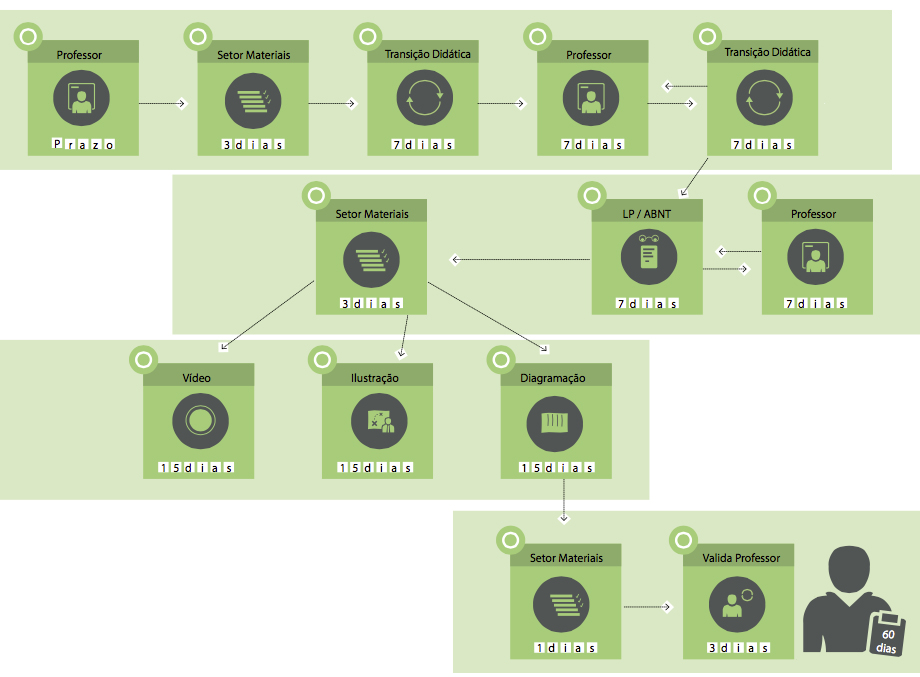
\includegraphics[width=1.0\textwidth]{Images/FluxoMateriaisNovos.jpg}
      \caption{Fluxo de Criação de Materiais Didáticos \\ Fonte: Setor de Produção Multimídia IMD - UFRN}
       \label{fig:fluxo_materiais_novos}
\end{figure}

A \hyperref[fig:fluxo_materiais_novos]{Figura \ref{fig:fluxo_materiais_novos}} descreve o fluxo para a criação do material didático de uma aula. Ele é iniciado com o envio do arquivo pelo autor para o setor de materiais, onde será feita uma primeira análise do conteúdo do material, o qual é então repassado para a equipe pedagógica responsável pela transição didática, processo de adaptar os conteúdos à perspectiva pedagógica da instituição. O material então fica alternando de responsabilidade entre o professor e a equipe pedagógica até que essa última determine a conformidade do conteúdo. Neste momento, a equipe de língua portuguesa e normas ABNT recebe o arquivo e se encarrega por executar revisões e melhorias juntamente com o professor, o resultado é encaminhado ao setor de materiais que, de acordo com as necessidades, solicita criação de material de vídeo, ilustração e, por último, diagramação, processo de organizar o material para publicação. Quando a equipe de diagramação termina seu trabalho, o arquivo volta à coordenação do setor de materiais para que seja feita uma nova verificação nos resultados obtidos e seja solicitada aprovação do professor que iniciou o processo.

No fluxo descrito, algumas equipes foram citadas, cada uma dessas está representada na \hyperref[fig:fluxo_materiais_novos]{Figura \ref{fig:fluxo_materiais_novos}} por um bloco e destaca um envolvido no processo, alguns deles são subsetores do setor de materiais e outros externos a esse. Na tabela abaixo é possível entender suas funções.

\begin{center}
\captionof{table}{Definição de envolvidos e papéis}
\begin{tabular}{|p{3cm}|p{11cm}|}
\hline            
\rowcolor[HTML]{EFEFEF}      
\textbf{Nome} & \textbf{Papel} \\ \hline
Gerência & É o responsável por receber e avaliar todas as demandas que chegam no setor, garantindo assim a execução do fluxo de produção, cumprimento dos prazos e a conformidade do material conforme solicitação.
\\ \hline 
Autor & Elabora o material didático textual, aulas/exercícios/provas, participando assim do fluxo de produção, de modo a ser realizando melhorias e possíveis correções textuais.             
\\ \hline 
Revisão Técnica & Garante a conformidade do conteúdo do material no ponto de vista técnico.
\\ \hline 
Transição Didática & Responsável por analisar a organização estrutural e didática da produção textual do autor, de modo que o conteúdo se adeque a linguagem adotada para um material de ensino a distância, de modo que o conteúdo esteja em conformidade com as necessidades pedagógicas do Instituto, podendo sugerir também alterações textuais e inserções multimídia de forma a tornar o material mais didático e atrativo.
\\ \hline                                                                                               
Revisão LP & Garante que as normas ortográficas e gramatical sejam atendidas, bem como o aperfeiçoamento do texto no que se refere a coerência e coesão, apresentando sugestões e orientações ao autor, tornando assim o texto mais claro e objetivo.
\\ \hline 
Revisão ABNT & Garante que as normas ABNT sejam aplicadas no conteúdo do material didático.    
\\ \hline       
Ilustração & Responsável pela parte gráfica e criação das imagens dos materiais.  
\\ \hline           
Vídeo & Responsável pela adequação do roteiro, gravação e edição de vídeos.    
\\ \hline                                                                                                                                         
Diagramação Web & Responsável pela inserção da aula no formato web, incluindo elementos responsivo e de interação. 
\\ \hline                                                                                                
Implementação Moodle & Responsável pela diagramação e publicação das atividades elaboradas pelo professor dentro do ambiente virtual de aprendizagem.
\\ \hline
Tipografia & Confere a versão final das aulas para garantir a ausência de erros na diagramação.
\\ \hline
\end{tabular}
\end{center}

\section{Situação Problema}

Os passos que compõem o fluxo existem com intuito de gerar resultados. Esses resultados representam um produto, um material que possui valor para o instituto. 

Tomando como exemplo o fluxo de materiais didáticos novos (ver \hyperref[fig:fluxo_materiais_novos]{Figura \ref{fig:fluxo_materiais_novos}}), na prática, os passos executados acontecem seguindo o processo a seguir:

\begin{enumerate}
  \item O autor envia os arquivos do material de aula à gerência do setor de materiais através de e-mail;
  \item Ao receber os arquivos, a equipe de gerência cria uma planilha com os dados do material, valida os documentos e passa para a equipe pedagógica;
  \item A equipe de pedagógica então executa a revisão textual e retorna para o autor caso seja necessário realizar ajustes. Esse ciclo se repete até que a equipe determine que o material está totalmente de acordo com as necessidades percebidas. Ao final, o material é enviado para a revisão de língua portuguesa e de normas ABNT;
  \item Os responsáveis pelas revisões LP/ABNT atuam sobre o material em conjunto com o autor até que os textos estejam em conformidade com as normas ortográficas e técnicas.
  \item O resultado do passo anterior é então encaminhado à gerência do setor que atualiza o estado do material na planilha e coordena os próximos passos. Neste momento, eles precisam determinar os elementos de audiovisual que são necessários para completar o produto. Essas necessidades resultam em solicitações para a equipe de vídeo, ilustração e, por último, diagramação. 
  \item Ao passo que a equipe de diagramação finaliza seu trabalho, há uma última verificação feita pela gerência e, então, todo o resultado retorna ao autor para a validação final.
\end{enumerate}

O passo-a-passo acima pode ser generalizado através do BPMN da figura a seguir.

\begin{figure}[H]
\centering
     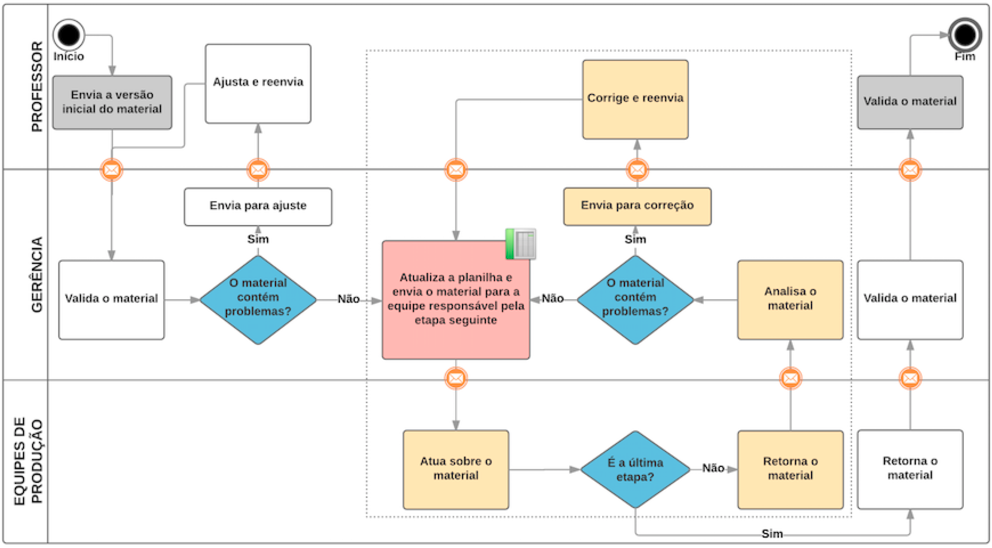
\includegraphics[width=1.0\textwidth]{Images/bpmn1.png}
      \caption{BPMN para Criação de Materiais Multimídia}
       \label{fig:bpmn1}
\end{figure}

No BPMN apresentado acima é possível entender melhor como o fluxo acontece. Nele, a gerência utiliza planilhas para administrar as versões do material e correio eletrônico para solicitações e conclusão das etapas. Em cada envio, a versão mais recente do material segue como anexo e, no corpo da mensagem, o direcionamento do que fazer e o prazo estipulado. Ao final do processo e dos e-mails trocados, o produto final se encontra pronto pra ser entregue aos alunos.

A forma como o processo descrito é executado representa a solução imediata encontrada pelos envolvidos para produção do material. Todavia, dado o estudo feito neste trabalho, é possível perceber que alguns pontos de falha se ressaltam nessa metodologia. 

Até o presente momento, foram citadas as utilizações de duas ferramentas importantes: o e-mail e a planilha. Como esses mecanismos não estão conectados diretamente, as suas utilizações implicam na necessidade de um forte mapeamento entre as solicitações e o acompanhamento da produção do material. Além disso, com a expansão das atividades e a elaboração de fluxos mais complexos, o número de envolvidos aumenta. Determinada equipe pode receber uma solicitação onde somente parte dos integrantes irá atuar sobre o material, o que gera outro nível de obrigação de controle, o interno da equipe. Por muitas vezes, os envolvidos precisam estar em contato direto, trocando informações e pedidos de maneira informal, o que descaracteriza o acompanhamento do método por parte da gerência. 

A perda de informação e registro causa não só a deficiência na execução quanto dificultam a criação de relatórios consistentes, pois há a necessidade de cruzamento manual de dados de diversas fontes. A equipe de gerência, responsável pela formação do material, tem o conhecimento prejudicado sobre o andamento do processo nas etapas das quais outras equipes são responsáveis. A ferramenta utilizada para as solicitações também pode facilitar a perda de prazos e de qualidade, visto que e-mails não propriamente enviados ou a não percepção do conteúdo que chega na caixa postal da equipe responsável pode acarretar em diminuição do tempo hábil para concretização do trabalho.

A contínua tarefa de verificação do recebimento do material e a necessidade de auditar o processo através de planilhas a parte dificultam a saída do material como o processo descrito acima teoriza. 

Determinados os pontos de falha, caracterizamos a situação problema encontrada como base para a especificação e desenvolvimento do corrente trabalho.

\section{Estado da Arte}

Sob o dever de executar o processo de produção dos materiais, o setor de materiais criou um mecanismo próprio que supre as necessidades e se mostra primordial para o estudo que foi realizado. É com base nesse mecanismo que se pode visualizar quais ferramentas poderiam ser agregadas com o objetivo de automatizar e dar suporte ao gerenciamento dos fluxos a fim de aumentar a qualidade do produto final. Algumas dessas ferramentas foram analisadas e suas possíveis formas de atuação serão descritas a seguir.

\subsection{Redmine}

O Redmine é um gerenciador de projeto flexível para web. Escrito usando Ruby on Rails e disponibilizado sob licença GPL, pode ser configurado para rodar em várias plataformas e suporta diversos bancos de dados. (MOURA; NASCIMENTO, 2010)

Como um gerenciador de projetos baseado na web, o Redmine possui ferramentas de acompanhamento de atividades que permite a atribuição de tarefas para usuários e equipes, o que se mostra bastante razoável no ponto de vista da necessidade principal do setor de materiais. 

Ao pensar no Redmine como uma ferramenta auxiliadora do processo em questão, percebe-se que, através de pequenas adaptações, é possível gerenciar a criação de materiais usando a abordagem de que cada etapa do fluxo seria representado por uma atividade. O setor de materiais seria responsável por criar as atividades e atribuir a cada envolvido responsável e, ao final de cada etapa, executaria o trabalho de transição de atividade para o próximo envolvido até que o material estivesse pronto.

Através da adaptação do processo pra ser usado dentro da ferramenta, é possível entender que essa se mostra interessante mas possui também suas limitações. Ao passo que precisa-se desvincular parte do trabalho de gerenciamento que é feito pelo setor de materiais, ao usar o Redmine, o setor ainda teria que estar intervindo a cada final de etapa e fazendo reatribuições ao longo do fluxo.

\subsection{Softwares baseados em Kanban}

Kanban é uma ferramenta inicialmente utilizada na metodologia \textbf{Just In Time}, desenvolvida e aperfeiçoada em 1940 pela Toyota. Essa metodologia descreve um sistema de administração produtivo baseado em produção sob demanda, ou seja, o estoque de matéria prima permanece mínimo e a fabricação é feita somente a tempo do produto ser entregue. O uso do Kanban nesse processo é realizado através de cartões sinalizadores que controlam o fluxo produtivo. No momento em que a demanda surge, um ou mais cartões são colocados em uma estrutura visual determinando a necessidade de produção e, após produção, os cartões são movidos para uma área que simboliza a concretização do pedido.

Um dos softwares baseados no Kanban é o Trello, um gerenciador de projetos e organizador de tarefas feito para a web. Nesta ferramenta, os projetos são representados por quadros, que contêm lista de tarefas e podem simbolizar fases do processo de produção. As tarefas são representadas por cartões e, no geral, possuem a descrição do que deve ser feito, o prazo de execução e os usuários responsáveis pela entrega.

No contexto de produção de materiais, os fluxos poderiam ser traduzidos como projetos e as etapas do fluxo seriam representadas pelas listas de tarefas, dessa maneira, os cartões de tarefa configurariam um material que poderia navegar pelo quadro através das etapas.

A partir do momento em que os cartões desse tipo de ferramenta são visualmente bem distribuídos, o uso para o processo de materiais traria um controle visual maior para a gerência. Todavia, determinada a necessidade do procedimento de produção depender do envio de documentos e do controle de versão desses, seria necessário utilizar uma ferramenta auxiliar para guardar esse tipo de dado visto que há limitações para arquivos com tamanhos elevados.

\section{Estrutura da Monografia}

No capítulo seguinte, o sistema será introduzido através da definição de seus requisitos, isto é, as propriedades e comportamentos percebidos que o produto deve atender. Na seção 2 do mesmo capítulo, os elementos de interface serão explicados juntamente com o estudo de interação entre eles e os usuários. Na seção seguinte, utilizaremos de diagramas e modelos para representar a definição dos componentes de software da arquitetura utilizada no desenvolvimento e, na última seção, mostraremos as telas explanando-as a fim de promover o entendimento fluxo de uso do sistema.

O capítulo 3 relata o estudo feito para análise do problema a ser resolvido pelo software desenvolvido. Nesse estudo, descrevemos a forma que os experimentos foram feitos juntamente com as equipes envolvidas no processo de produção de materiais e como os resultados obtidos influenciaram nas melhorias do produto.

Por fim, o capítulo 4 narra as  conclusões obtidas durante o planejamento e execução da produção deste trabalho. Trabalhos futuros e expectativas do autor para a solução também agregam a este capítulo.

%\section{Proposta}
%
%Como proposta do estudo feito, surge o desenvolvimento do Sistema de Materiais - SiMate, um produto modelado juntamente com todos os usuários e demais envolvidos no processo de criação de materiais.
%
%O SiMate tem como principal diferencial o fato de ser feito totalmente sob medida para solucionar os problemas encontrados no mecanismo atual de produção. A ferramenta aqui apresentada trás consigo todas as funcionalidades que o método usado oferece, juntamente com as soluções que outras ferramentas oferecem e melhorias que os usuários poderão perceber ao longo do tempo. Tudo isso unificado em um sistema totalmente extensível e proprietário.
%
%Algumas das necessidades de mais importância levantados na fase de elicitação de requisitos são o versionamento de alteração do material no processo de criação, a definição de papeis para as equipes, a geração de relatórios, a auditoria do fluxo produtivo - o que permite que todos saibam exatamente a etapa atual que a atividade se encontra, o calendário de deadlines, sistema de notificações, definição de prioridades dos produtos e registro de alterações. Estas funcionalidades serão melhor descritas na seção \hyperref[subsec:requisitos_funcionais]{\ref{subsec:requisitos_funcionais}}
%
%Todas esses requisitos serão melhor contextualizados, conceituados e exemplificados no decorrer do estudo.

%

%
%\subsection{Objetivos}
%
%Os objetivos desse trabalho são descrever em detalhes o processo de criação de materiais pelo setor de materiais do IMD, encontrar e interpretar a situação problema, definir formas de operação mais eficientes, projetar um mecanismo de software que atenda as novas definições, desenvolver e experimentar a solução proposta. Além disso, o resultado aqui obtido deve não só documentar o projeto, mas também servir de base para a evolução e manutenção do sistema pela equipe responsável.
%
%\subsection{Metodologia}
%
%Como um dos objetivos principais desse trabalho é descrever um processo, adiciona-se a esta pesquisa o teor descritivo. De acordo com Selltiz et al. (1965), a pesquisa descritiva busca descrever um fenômeno ou situação em detalhe, especialmente o que está ocorrendo, permitindo abranger, com exatidão, as características de um indivíduo, uma situação, ou um grupo, bem como desvendar a relação entre os eventos. 
%
%E, ao passo que o estudo feito contempla a análise, teorização de novas formas de execução, projeto de um mecanismo com base nas teorias, desenvolvimento e experimento, pode-se caracterizar essa pesquisa explicativa-experimental.
%
%Entendido a metodologia quanto aos objetivos, nas próximas seções serão explanados os procedimentos utilizados no estudo e como a abordagem do problema foi feita.
%
%\subsection{Metodologia}
%
%
%\subsubsection{Procedimentos}
%
%Os procedimentos utilizados para entendimento do processo como um todo foram, inicialmente, observação direta da execução do fluxo de criação de materiais. Posteriormente, o levantamento de requisitos foi feito e validado com o setor.
%
%As técnicas utilizadas para levantamento de requisitos se caracterizam como: a) compreensão do domínio, onde o responsável pelo estudo desenvolve o entendimento a partir do contato com o ambiente da aplicação; b) coleta de requisitos, processo em que o analista descobre os requisitos partindo da compreensão do domínio; c) classificação e organização, essa atividade contempla a divisão dos requisitos em grupos de afinidades; d) definição de prioridades, aqui os envolvidos são consultados para que haja a determinação dos requisitos mais importantes; e) verificação e resolução de conflitos, neste último passo os requisitos são verificados para garantir a completude, consistência e se estão em concordância com os envolvidos.
%
%Dados os requisitos, a especificação dos principais é feita através do detalhamento dos cenários de interação entre os usuários e o sistema, atividade também chamada de expansão de casos de uso. Essa expansão busca trazer clareza do fluxo para que todos os eventuais leitores possam entendê-lo de igual forma.
%
%

	
	% Capitulo 2: Gema
	
\chapter{Gema: Gestão de Produção Multimídia}

Gema foi o nome escolhido para o sistema de gestão de produção multimídia desenvolvido com o propósito de sanar as necessidades do processo aqui estudado. Acentuar a visibilidade de cada estado do fluxo, enfatizar a comunicação entre os usuários, administrar e notificar os prazos de entrega e controlar as versões dos materiais são funcionalidades incorporadas ao projeto. 

A seguir entenderemos de forma mais sistemática os requisitos para o desenvolvimento e aprenderemos como usar o Gema.

\section{Elicitação de Requisitos}

Durante o estudo feito, os requisitos do sistema foram elicitados e, nesta seção, estão divididos em regras de negócios, requisitos funcionais e requisitos não funcionais.

\subsection{Regras de Negócio} \label{subsec:regras_de_negocio}

As regras de negócio definem as instruções de como o sistema irá atingir o seu objetivo obedecendo as políticas internas e definições básicas de conduta da instituição ou organização dona do produto.

Nesta subseção serão definidas as restrições, validações, condições e exceções que fazem parte do conjunto de rotinas contempladas pelo sistema desenvolvido.

\begin{enumerate}[label=\textbf{RN\protect\twodigits{\theenumi}}, leftmargin=2cm]
	
	% ADMIN
	\item \label{rn:role_admin_permissions} Usuários com papel de Administrador devem possuir acesso total às funcionalidades do sistema. \\
		\textbf{Prioridade:} Alta \\
		\textbf{Depende de:} Nenhum

	\item \label{rn:role_admin_exclusion_permissions} Somente os usuários com papel de Administrador podem executar a exclusão de dados do sistema. \\
		\textbf{Prioridade:} Alta \\
		\textbf{Depende de:} \hyperref[rn:role_admin_permissions]{\ref{rn:role_admin_permissions}}
	
	% MANAGEMENT
	\item \label{rn:role_management_permissions} Usuários com papel Gerência devem possuir acesso total às funcionalidades do sistema com exceção das ações de exclusão. \\
		\textbf{Prioridade:} Alta \\
		\textbf{Depende de:} Nenhum

	% ADMIN & MANAGEMENT
	\item \label{rn:material_files_visibility} Administrador e Gerência devem ser os únicos papéis a terem acesso aos arquivos das versões anteriores de um material. Usuários sem um desses papéis somente podem interagir com os arquivos do material no momento em que o fluxo de produção estiver em sua responsabilidade. \\
		\textbf{Prioridade:} Alta \\
		\textbf{Depende de:} Nenhum

	% AUTHOR
	\item \label{rn:role_author_permissions} Somente usuários com papel de Autor devem poder participar do grupo de responsáveis por uma oferta de disciplina e incluir a primeira versão de um material. \\
		\textbf{Prioridade:} Alta \\
		\textbf{Depende de:} Nenhum

	\item \label{rn:role_author_permissions2} O sistema deve limitar o acesso dos usuários com papel de Autor somente às ofertas de disciplina em que os mesmos pertençam ao grupo de responsáveis. \\
		\textbf{Prioridade:} Média \\
		\textbf{Depende de:} \hyperref[rn:role_author_permissions]{\ref{rn:role_author_permissions}}

	% FLOW
	\item \label{rn:flow} É obrigatória a inserção de arquivo ou comentário explicativo na etapa inicial do fluxo do material por parte do usuário responsável pela oferta da disciplina (Autor). \\
		\textbf{Prioridade:} Alta \\
		\textbf{Depende de:} \hyperref[rn:role_author_permissions]{\ref{rn:role_author_permissions}} e \hyperref[rn:role_author_permissions2]{\ref{rn:role_author_permissions2}}
				
	\item \label{rn:flow2} Com exceção da etapa inicial do fluxo de produção, usuários com papel de Administrador ou Gerência podem atuar sobre o material em quaisquer circunstância, conseguindo avançar as etapas ou finalizar o fluxo a qualquer momento. \\
		\textbf{Prioridade:} Alta \\
		\textbf{Depende de:} \hyperref[rn:flow]{\ref{rn:flow}}

	\item \label{rn:flow3} Nas etapas subsequentes a inicial do fluxo de produção, somente usuários com o papel referente ao sinalizado pela corrente etapa podem atuar sobre o material (salvo \hyperref[rn:flow2]{\ref{rn:flow2}}). \\
		\textbf{Prioridade:} Alta \\
		\textbf{Depende de:} \hyperref[rn:flow2]{\ref{rn:flow2}}

	\item \label{rn:flow4} Com exceção da etapa inicial do fluxo de produção, deve sempre haver a possibilidade do usuário responsável pela etapa atual direcionar o material ao grupo de autores ou ao grupo de gerência. Esses comportamentos devem existir para caso haja a necessidade dos autores executarem correções ou a equipe de gerência realizar procedimentos de controle ou solucionar problemas não especificados. \\
		\textbf{Prioridade:} Alta \\
		\textbf{Depende de:} Nenhum

	\item \label{rn:flow5} No momento em que o material chega a etapa final do fluxo de produção, o usuário com o papel responsável deve poder inicializar a finalização do processo com os seguintes passos: \\
		1 - O usuário responsável pela etapa final sinaliza o término do fluxo de produção, o sistema então direciona o material para validação por parte dos autores; \\
		2 - Os autores avaliam e validam o produto, direcionando-o à equipe de gerência para finalização; \\
		3 - A equipe de gerência recebe o material e executa a última verificação, encerrando o fluxo de produção. \\
		\textbf{Prioridade:} Alta \\
		\textbf{Depende de:} Nenhum

\end{enumerate}

\subsection{Requisitos Funcionais} \label{subsec:requisitos_funcionais}
		
Requisitos funcionais são necessidades funcionais que devem ser oferecidas e que definem o comportamento perceptível do sistema por parte dos usuários.		

Para facilitar o entendimento e evitar repetições, a sigla CRUD (acrónimo de Create, Read, Update e Delete na língua Inglesa) será usada como representação das ações de criação, visualização, edição e exclusão do modelo ao qual estiver referenciando.

\begin{enumerate}[label=\textbf{RF\protect\twodigits{\theenumi}}, leftmargin=2cm]

	\item \label{rf:users} Gerenciar usuários \\
		\textbf{Descrição:} O sistema deve permitir o gerenciamento dos usuários através das ações de CRUD. \\
		\textbf{Prioridade:} Alta \\
		\textbf{Depende de:} Nenhum

	\item \label{rf:steps} Gerenciar etapas \\
		\textbf{Descrição:} O sistema deve permitir o gerenciamento de etapas através das ações de CRUD. \\
		Etapas representam estados que o material pode se encontrar durante a execução do fluxo de produção, cada uma delas deve estar relacionada a um grupo de papéis, dessa maneira, somente usuários pertencentes ao grupo podem atuar sobre o material no momento da sua execução. \\
		\textbf{Prioridade:} Alta \\
		\textbf{Depende de:} Nenhum

	\item \label{rf:flows} Gerenciar fluxos \\
		\textbf{Descrição:} O sistema deve permitir o gerenciamento de fluxos através das ações de CRUD. \\
		O fluxo possui etapa inicial, etapas intermediárias e etapa final. As etapas do fluxo devem se conectar umas com as outras formando uma estrutura coesa onde, a partir da inicial, possa se chegar a final. \\
		O sistema deve permitir que, ao transitar pelas etapas intermediárias do fluxo, haja a possibilidade de mais de um caminho percorrível e possíveis laços ligando duas ou mais etapas. \\
		\textbf{Prioridade:} Alta \\
		\textbf{Depende de:} \hyperref[rf:steps]{\ref{rf:steps}}

	\item \label{rf:artifact_types} Gerenciar tipos de artefatos \\
		\textbf{Descrição:} O sistema deve permitir o gerenciamento de tipos de artefato através das ações de CRUD. \\
		Artefato é o nome dado a um agrupamento de materiais, tipos básicos de artefatos são aula e prova. O objetivo deste modelo é tornar dinâmicos os tipos de artefatos a serem usados no sistema. \\
		\textbf{Prioridade:} Alta \\
		\textbf{Depende de:} Nenhum
				
	\item \label{rf:subjects} Gerenciar disciplinas \\
		\textbf{Descrição:} O sistema deve permitir o gerenciamento de disciplinas através das ações de CRUD. \\
		Este modelo define o conjunto de possíveis disciplinas a serem ofertadas no sistema. \\
		Como exemplo, imaginaremos a necessidade de ofertar a disciplina Estrutura de Dados II, uma das configurações obrigatórias é o registro da disciplina com o título escolhido. \\
		\textbf{Prioridade:} Alta \\
		\textbf{Depende de:} Nenhum

	\item \label{rf:modules} Gerenciar módulos \\ 
		\textbf{Descrição:} O sistema deve permitir o gerenciamento de módulos através das ações de CRUD. \\
		O módulo representa um período de tempo com datas de início e fim, semestre ano. \\
		Este modelo será usado de forma combinada com os registros de disciplina na oferta (ver \hyperref[rf:offers]{\ref{rf:offers}}). \\
		Aperfeiçoando o exemplo iniciado no \hyperref[rf:subjects]{\ref{rf:subjects}}, iremos imaginar a necessidade de ofertar a disciplina Estrutura de Dados II nos períodos de 2016.1 e 2017.1, ambos com datas de início e fim correspondentes as do semestre. Essa necessidade torna obrigatória tanto a configuração da disciplina quanto o registro dos módulos que contemplem os dois períodos escolhidos. \\
		\textbf{Prioridade:} Alta \\
		\textbf{Depende de:} Nenhum
		
	\item \label{rf:offers} Gerenciar ofertas \\
		\textbf{Descrição:} O sistema deve permitir o gerenciamento de ofertas através das ações de CRUD. \\
		As ofertas designam, de fato, a execução das disciplinas em períodos de tempo (módulos). Cada registro desse modelo deve possuir um grupo de artefatos (aulas, provas, etc.) cuja responsabilidade é dos autores. \\
		Os artefatos  devem ser definidos com datas máximas para início e fim do fluxo de produção de seus materiais. \\
		O que determina como o processo de produção de um material ocorrerá é a associação dele com um fluxo previamente cadastrado (ver \hyperref[rf:flows]{\ref{rf:flows}}). \\
		Continuando com o exemplo do \hyperref[rf:modules]{\ref{rf:modules}}, incrementamos o cenário da seguinte maneira: a disciplina Estrutura de Dados II que ocorrerá nos períodos de 2016.1 e 2017.1 deve possuir 20 aulas e 3 provas, cada aula com os materiais de texto base e lista de questões, e cada prova com o arquivo de prova. Dadas as especificações, o modelo permitirá a criação ofertas de disciplina para os módulos que contemplem os períodos escolhidos com os artefatos indicados. \\
		\textbf{Prioridade:} Alta \\
		\textbf{Depende de:} \hyperref[rf:flows]{\ref{rf:flows}}, \hyperref[rf:artifact_types]{\ref{rf:artifact_types}}, \hyperref[rf:subjects]{\ref{rf:subjects}} e \hyperref[rf:modules]{\ref{rf:modules}}
		
	
			
	\item \label{rf:init_flow} Iniciar fluxo de material \\ 
		\textbf{Descrição:} Para todo material deverá ser possível que um dos autores responsáveis pela oferta submeta sua primeira versão iniciando assim o fluxo de produção. Deverá ser aceito como primeira versão arquivo ou comentário explicativo.  \\
		Após submissão, o material deverá encontrar-se na etapa inicial do fluxo onde os responsáveis por esse passo estarão encarregados de continuar o processo de criação. \\
		\textbf{Prioridade:} Alta \\
		\textbf{Depende de:} \hyperref[rf:offers]{\ref{rf:offers}}

	\item \label{rf:assignTask} Assumir tarefa \\ 
		\textbf{Descrição:} Cada etapa do fluxo de produção possui uma ou mais tarefas a serem resolvidas. O sistema deverá permitir que o usuário com o papel designado para resolução da tarefa sinalize a sua responsabilidade. \\
		Após assumir a tarefa, outros usuários são impossibilitados de resolver a mesma. \\
		\textbf{Prioridade:} Alta \\
		\textbf{Depende de:} \hyperref[rf:steps]{\ref{rf:steps}} e \hyperref[rf:offers]{\ref{rf:offers}}

	\item \label{rf:unassignTask} Revogar tarefa \\ 
		\textbf{Descrição:} Após assumir uma tarefa, o usuário responsável deve poder desistir da mesma. Ao realizar essa ação, a tarefa volta a estar disponível para que outros usuário a assumam. \\
		Usuários com papel de Administrador ou Gerência devem poder remover a responsabilidade do dono de qualquer tarefa. \\
		\textbf{Prioridade:} Alta \\
		\textbf{Depende de:} \hyperref[rf:assignTask]{\ref{rf:assignTask}}

	\item \label{rf:solveTask} Resolver tarefa \\ 
		\textbf{Descrição:} Ao assumir a tarefa, o sistema deve possibilitar que o usuário a resolva. A atividade a ser executada deve ser comunicada ao usuário a partir dos dados descritivos da tarefa anteriormente cadastrada. \\
		A forma de resolução é através de arquivo ou comentário explicativo. \\
		Ao passo que for resolvida, o sistema deve contabilizar a porcentagem que a tarefa representa no total da etapa. \\
		\textbf{Prioridade:} Alta \\
		\textbf{Depende de:} \hyperref[rf:assignTask]{\ref{rf:assignTask}}

	\item \label{rf:endStep} Finalizar etapa e direcionar material para próxima etapa \\
		\textbf{Descrição:} Após a resolução de todas as tarefas de uma etapa, o sistema deverá permitir que os usuários responsáveis por quaisquer das tarefas resolvidas a finalize. \\
		A finalização da etapa compreende na possibilidade de direcionar o material à próxima etapa. As etapas possíveis devem refletir a determinação feita na criação do fluxo. \\
		\textbf{Prioridade:} Alta \\
		\textbf{Depende de:} \hyperref[rf:flows]{\ref{rf:flows}} e \hyperref[rf:solveTask]{\ref{rf:solveTask}}

	\item \label{rf:endStepWithCorrection} Finalizar etapa e direcionar material para correção \\ 
		\textbf{Descrição:} Após a resolução de todas as tarefas de uma etapa, o sistema deverá permitir que usuários responsáveis por quaisquer das tarefas resolvidas a finalize. \\
		A finalização da etapa deve possibilitar o direcionamento do material para correção pelos autores da oferta. \\
		\textbf{Prioridade:} Alta \\
		\textbf{Depende de:} \hyperref[rf:flows]{\ref{rf:flows}} e \hyperref[rf:solveTask]{\ref{rf:solveTask}}

	\item \label{rf:endCorrection} Finalizar correção do material \\ 
		\textbf{Descrição:} Após direcionamento do material para correção, uma tarefa é aberta na responsabilidade dos autores da oferta. \\
		A resolução da tarefa define o retorno do material para a etapa que anteriormente o enviou para correção. \\
		\textbf{Prioridade:} Alta \\
		\textbf{Depende de:} \hyperref[rf:endStepWithCorrection]{\ref{rf:endStepWithCorrection}}

	\item \label{rf:endStepWithManagement} Finalizar etapa e direcionar material à gerência \\ 
		\textbf{Descrição:} Após resolução de todas as tarefas de uma etapa, o sistema deverá permitir que usuários responsáveis por quaisquer das tarefas resolvidas a finalize. \\
		A finalização de qualquer etapa deve possibilitar o direcionamento do material para que a equipe de gerência realize procedimentos de controle ou solucione problemas não especificados. \\
		\textbf{Prioridade:} Alta \\
		\textbf{Depende de:} \hyperref[rf:solveTask]{\ref{rf:solveTask}}

	\item \label{rf:endCorrection} Finalizar gerenciamento do material \\ 
		\textbf{Descrição:} Após direcionamento do material à gerência, uma tarefa é aberta na responsabilidade dessa equipe. \\
		O sistema deverá permitir que, após resolução da tarefa, o material possa ser enviado para quaisquer etapa do fluxo ou para os autores da oferta. \\
		\textbf{Prioridade:} Alta \\
		\textbf{Depende de:} \hyperref[rf:endStepWithManagement]{\ref{rf:endStepWithManagement}}

	\item \label{rf:endStepAndFlow} Finalizar etapa e fluxo \\ 
		\textbf{Descrição:} Após a resolução de todas as tarefas de uma etapa, o sistema deverá permitir que usuários responsáveis por quaisquer das tarefas resolvidas a finalize. \\
		O finalização da etapa final do fluxo possibilita que o usuário encerre também o fluxo de produção. Essa ação determina o início do processo de validação e fechamento do material. \\
		\textbf{Prioridade:} Alta \\
		\textbf{Depende de:} \hyperref[rf:solveTask]{\ref{rf:solveTask}}

	\item \label{rf:validateMaterial} Validar material \\ 
		\textbf{Descrição:} Após finalização do fluxo, os autores da oferta são encarregados de validar o material produzido. \\
		A validação determina a responsabilidade da equipe de gerência pelo encerramento do material. \\
		\textbf{Prioridade:} Alta \\
		\textbf{Depende de:} \hyperref[rf:endStepAndFlow]{\ref{rf:endStepAndFlow}}

	\item \label{rf:completeMaterial} Encerrar material \\ 
		\textbf{Descrição:} Após validação, o sistema deve possibilitar que a equipe de gerência execute o último passo para a finalização do material. \\
		A finalização do material encerra o seu processo de criação. Após isso, a última versão do material deve ser disponibilizada como produto final. \\
		\textbf{Prioridade:} Alta \\
		\textbf{Depende de:} \hyperref[rf:validateMaterial]{\ref{rf:validateMaterial}}

	\item \label{rf:newOfferNotification} Notificar oferta cadastrada \\ 
		\textbf{Descrição:} Ao passo que houver o cadastro de uma nova oferta, o sistema deverá notificar o grupo de autores responsáveis do ocorrido. \\
		\textbf{Prioridade:} Média \\
		\textbf{Depende de:} \hyperref[rf:offers]{\ref{rf:offers}}

	\item \label{rf:deliveryNotification} Notificar prazo de entrega do material \\ 
		\textbf{Descrição:} O sistema deverá notificar os autores da oferta quando os materiais não iniciados estiverem com a data próxima a estimada para entrega. \\
		\textbf{Prioridade:} Média \\
		\textbf{Depende de:} \hyperref[rf:offers]{\ref{rf:offers}}

	\item \label{rf:deliveryDelayNotification} Notificar atraso na entrega do material \\ 
		\textbf{Descrição:} O sistema deverá notificar diariamente os autores da oferta quando houver materiais com o prazo de entrega ultrapassado.  \\
		\textbf{Prioridade:} Média \\
		\textbf{Depende de:} \hyperref[rf:offers]{\ref{rf:offers}}

	
\end{enumerate}

\subsection{Requisitos Não-Funcionais}

\begin{enumerate}[label=\textbf{RNF\protect\twodigits{\theenumi}}, leftmargin=2cm]

	\item \label{rf:papeis} O sistema deve estar disponível 24 horas/dia e 7 dias/semana, a fim de garantir que as metas estabelecidas para criação dos materiais não sejam quebradas por indisponibilidade da aplicação. \\
		\textbf{Categoria:} Disponibilidade e Confiabilidade \\
		\textbf{Escopo:} Sistema \\
		\textbf{Prioridade:} Alta \\
		\textbf{Depende de:} Nenhum

	\item \label{rf:papeis} O sistema deve lidar com os vários níveis de acesso dos usuários restringindo a interação com os conteúdos a eles associados. \\
		\textbf{Categoria:} Segurança de Acesso \\
		\textbf{Escopo:} Funcionalidade \\
		\textbf{Prioridade:} Alta \\
		\textbf{Depende de:} Nenhum

	\item \label{rf:papeis} O sistema deve trazer uma interface amigável, simples, rápida e eficiente. \\
		\textbf{Categoria:} Usabilidade, Atratividade e Desempenho \\
		\textbf{Escopo:} Sistema \\
		\textbf{Prioridade:} Alta \\
		\textbf{Depende de:} Nenhum

	\item \label{rf:papeis} Para garantir a fácil manutenção pela equipe a qual será entregue o sistema após o desenvolvimento, esse deve ser implementado utilizando a linguagem de programação JAVA. \\
		\textbf{Categoria:} Implementação \\
		\textbf{Escopo:} Sistema \\
		\textbf{Prioridade:} Alta \\
		\textbf{Depende de:} Nenhum

\end{enumerate}

%\section{Especificação de Casos de Uso}
%
%Nesta seção serão especificados as unidades funcionais que representam as necessidades principais do sistema. No primeiro tópico, os atores participantes dessas funcionalidades serão conceituados e, após isso, será feito o detalhamento dos casos de uso.
%
%\subsection{Atores}
%
%\subsubsection{Administrador}
%
%O ator Administrador representa a pessoa que tem poder total sobre o sistema. Nenhuma funcionalidade é restringida a esse tipo de usuário.
%
%\subsubsection{Setor de Materiais}
%
%No sistema, o usuário possuidor do papel de Setor de Materiais é responsável principalmente por gerir a execução do fluxo, permitindo assim auditoria e intervenção no processo.
%
%\subsubsection{Membro}
%
%O ator Membro existe para representar usuários como o professor e os membros das demais equipes no sistema. O principal objetivo desse tipo de usuário é participar do fluxo de materiais contribuindo para que o material seja desenvolvido.
%
%\subsection{Casos de Uso}
%     
%\begin{enumerate}[label=\textbf{UC01}, leftmargin=2cm]
%	\item \textbf{Criar Etapa} \\
%	A etapa representa um possível passo em qualquer fluxo, dessa forma, cada etapa pode participar de diversos fluxos ao mesmo tempo, sendo a ela atribuído somente nome, responsáveis e descrição. \\
%	\begin{minipage}[c]{10cm}
%	    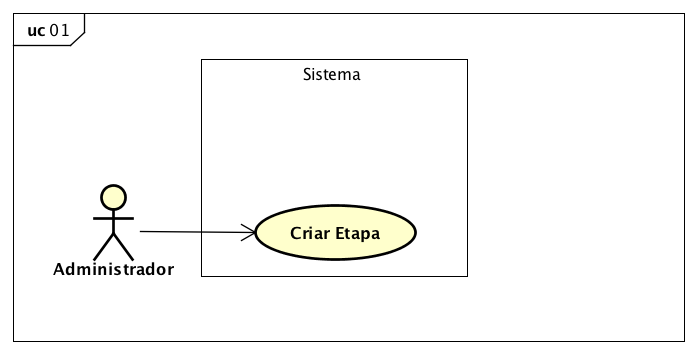
\includegraphics[width=10cm]{Imagens/UC_CriarEtapa.png}
%	    \captionof{figure}{Diagrama do Caso de Uso Criar Etapa}
%		\label{fig:uc_criar_fluxo}
%	\end{minipage} \\
%
%	\begin{enumerate}[label=, leftmargin=0cm]
%		\item \textbf{Atores} \\
%		Administrador
%		\item \textbf{Precondições}
%			\begin{enumerate}[label=\arabic*.]
%				\item Usuário estar logado no sistema.
%			\end{enumerate}
%		\item \textbf{Fluxo Básico}
%			\begin{enumerate}[label=\arabic*.]
%				\item Usuário solicita o formulário de criação de etapa.
%				\item O sistema exibe formulário onde o usuário deve preencher o nome da etapa, os papéis pela execução da etapa e uma descrição.
%				\item Usuário preenche formulário.
%				\item O sistema valida os dados e informa que o fluxo com salvo com sucesso.
%			\end{enumerate}
%		\item \textbf{Pós-condições}
%			\begin{enumerate}[label=\arabic*.]
%				\item Uma nova etapa foi criada e pode ser visualizado, editado, excluído ter passos do fluxo associados a ela.
%			\end{enumerate}
%	\end{enumerate}
%	 
%\end{enumerate}
%
%\begin{enumerate}[label=\textbf{U02}, leftmargin=2cm]
%	\item \textbf{Criar Fluxo} \\
%	Este caso de de uso detalha a elaboração do fluxo e suas etapas. No sistema, um fluxo criado representa o passo-a-passo para a criação dos materiais associados. \\
%	\begin{minipage}[c]{10cm}
%	    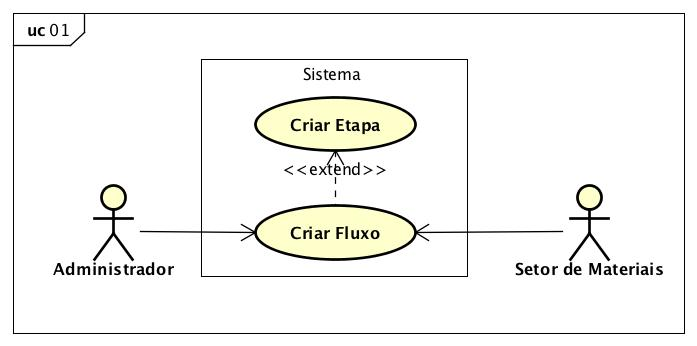
\includegraphics[width=10cm]{Imagens/UC_CriarFluxo.jpg}
%	    \captionof{figure}{Diagrama do Caso de Uso Criar Fluxo}
%		\label{fig:uc_criar_fluxo}
%	\end{minipage} \\
%
%	\begin{enumerate}[label=, leftmargin=0cm]
%		\item \textbf{Atores} \\
%		Administrador e Setor de Materiais
%		\item \textbf{Precondições}
%			\begin{enumerate}[label=\arabic*.]
%				\item Usuário estar logado no sistema.
%			\end{enumerate}
%		\item \textbf{Fluxo Básico}
%			\begin{enumerate}[label=\arabic*.]
%				\item Usuário solicita o formulário de criação de fluxo.
%				\item O sistema exibe formulário onde o usuário deve preencher o nome do fluxo, definir os possíveis caminhos que o fluxo pode tomar a partir das etapas e, por último, definir etapa final e inicial.
%				\item Usuário preenche formulário.
%				\item O sistema valida os dados e informa que o fluxo foi salvo com sucesso.
%			\end{enumerate}
%		\item \textbf{Fluxo Alternativo A}
%			\begin{enumerate}[label=\arabic*.]
%				\item No passo 2 do Fluxo Básico, o sistema não retorna etapas anteriormente criadas e/ou o usuário de tipo Administrador decide criar uma nova etapa para ser usada no fluxo. 
%				\item Usuário solicita formulário de criação de etapa.
%				\item Sistema exibe formulário onde o usuário deve preencher o nome da etapa, os responsáveis e uma descricão.
%				\item Usuário preenche o formulário.
%				\item Sistema valida, informa que a etapa foi criada e retorna ao passo 2 do Fluxo Básico.
%			\end{enumerate}
%		\item \textbf{Fluxo Alternativo B}
%			\begin{enumerate}[label=\arabic*.]
%				\item No passo 4 do Fluxo Básico, o sistema invalida o formulário por falta de informação e/ou os passos do fluxo não estão consistentes.
%				\item O sistema informa os erros presentes no formulário e solicita que o usuário corrija os erros.
%				\item Volta ao passo 3 do Fluxo Básico.
%			\end{enumerate}
%		\item \textbf{Pós-condições}
%			\begin{enumerate}[label=\arabic*.]
%				\item Um novo fluxo foi criado e pode ser visualizado, editado, excluído e associado à materiais.
%			\end{enumerate}
%	\end{enumerate}
%	 
%\end{enumerate}
%
%\begin{enumerate}[label=\textbf{UC03}, leftmargin=2cm]
%	\item \textbf{Criar Material} \\
%	Este caso de uso detalha o processo de criação do material. Para elaboração do material, um fluxo bem definido e consistente deve ser associado.  \\
%	\begin{minipage}[c]{10cm}
%	    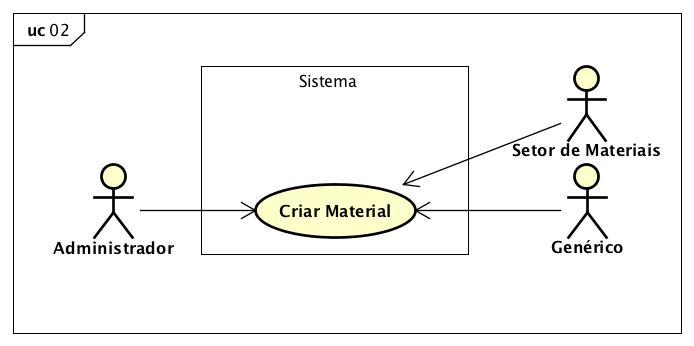
\includegraphics[width=10cm]{Imagens/UC_CriarMaterial.jpg}
%	    \captionof{figure}{Diagrama do Caso de Uso Criar Material}
%		\label{fig:uc_criar_material}
%	\end{minipage} \\
%
%	\begin{enumerate}[label=, leftmargin=0cm]
%		\item \textbf{Atores} \\
%		Administrador, Setor de Materiais e Genérico.
%		\item \textbf{Precondições}
%			\begin{enumerate}[label=\arabic*.]
%				\item Existir oferta cadastrada com módulo e disciplina.
%				\item Existir artefato de aula ou prova relacionado com a oferta.
%				\item Existir um fluxo associado ao artefato.
%				\item Usuários responsáveis pelas etapas do fluxo estarem logados no sistema.
%			\end{enumerate}
%		\item \textbf{Fluxo Básico}
%			\begin{enumerate}[label=\arabic*.]
%				\item Usuário solicita visualização da oferta.
%				\item Sistema exibe dados da oferta com todos os artefatos (aula ou prova).
%				\item Usuário seleciona artefato que deseja dar início ao processo de criação do material.
%				\item Sistema exibe formulário de criação do material com campos para carregamento do arquivo, mensagem e possíveis próximas etapas para as quais esse material pode seguir.
%				\item Usuário preenche o formulário, carrega o arquivo e define qual o próximo passo do fluxo.
%				\item Sistema recebe os dados, informa ao usuário que o material foi submetido.
%				\item Sistema notifica responsáveis pela etapa atual do material e aguarda ação.
%				\item Usuário responsável pela etapa atual solicita visualização do material.
%				\item Sistema exibe informações do material atual permitindo que o usuário baixe o arquivo.
%				\item Usuário solicita criação de nova versão do material atual.
%				\item Sistema mostra formulário de criação de nova versão do material atual com campos para carregamento do arquivo, mensagem e possíveis próximas etapas para as quais esse material pode seguir.
%				\item Usuário preenche o formulário, carrega o arquivo e define qual o próximo passo do fluxo.
%				\item Volta ao passo 6 e repete até que o material chegue à etapa final do fluxo.
%				\item Sistema sinaliza que o fluxo do artefato foi completado e que o material está pronto.
%			\end{enumerate}
%		\item \textbf{Fluxo Alternativo A}
%			\begin{enumerate}[label=\arabic*.]
%				\item Ao fim do passo 2 do Fluxo básico, um usuário com papel de Administrador decide interver no fluxo e move o material para alguma etapa que não é necessariamente uma das disponíveis a partir da etapa atual.
%				\item O fluxo retorna ao passo 13 do Fluxo Básico.
%			\end{enumerate}
%		\item \textbf{Pós-condições}
%			\begin{enumerate}[label=\arabic*.]
%				\item O estado de feito é atribuído ao artefato do material.
%				\item Há um material pronto e disponível.
%			\end{enumerate}
%	\end{enumerate}
%	 
%\end{enumerate}

\section{Projeto de Interface}

O projeto de interface define o conjunto de requisitos e ações de interface que permitem o usuário realizar os procedimentos do sistema de modo a satisfazer as metas de usabilidade definidas. A abstração promovida por esse estudo busca antecipar a percepção de incoerências e melhorar a qualidade da elicitação e detalhamento dos requisitos.

A técnica de elaboração de \textit{wireframes} foi usada para sugerir a interface do sistema a ser desenvolvido. \textit{Wireframes} são protótipos estruturais usados para simular páginas e mecanismos de navegação.

Os primeiros \textit{wireframes} (Figuras \hyperref[fig:wf_dashboard]{\ref{fig:wf_dashboard}} e \hyperref[fig:wf_dashboard_admin]{\ref{fig:wf_dashboard_admin}}) demonstram as telas inicias para usuários não-administradores e administradores. Em ambos os protótipos, pode-se perceber a presença dos seguintes elementos:

\begin{enumerate}  
\item Barra de navegação: é composta pelos mecanismos básicos para navegação na aplicação. Esse elemento normalmente permanece presente em todas as telas e se dispõe na parte superior ou à esquerda da tela.
\item Caixa de alertas: esta seção representa a necessidade da apresentação em trazer para primeiro plano os alertas de atrasos na entrega e finalização dos materiais;
\item Caixa de mensagens: revela o dever do sistema em possuir mecanismos para a comunicação entre os usuários.
\end{enumerate}

\vspace{5mm}
\begin{minipage}[c]{\textwidth}
    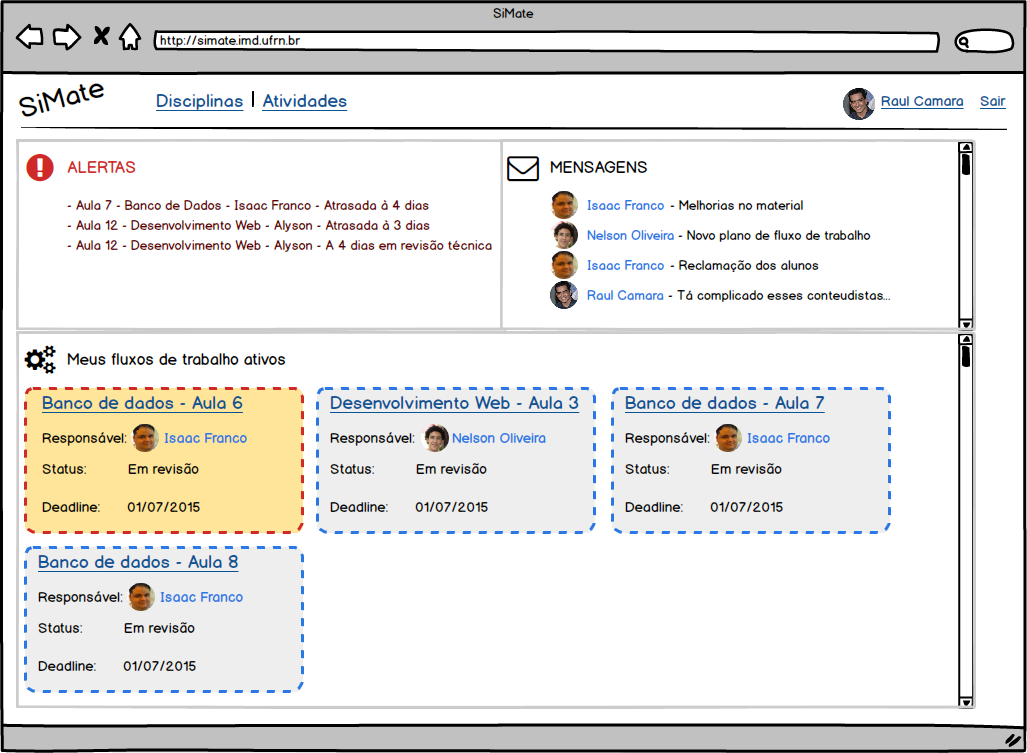
\includegraphics[width=15cm]{Wireframes/Dashboard.png}
    \captionof{figure}{Tela Inicial}
	\label{fig:wf_dashboard}
\end{minipage} \\

\vspace{5mm}
\begin{minipage}[c]{\textwidth}
    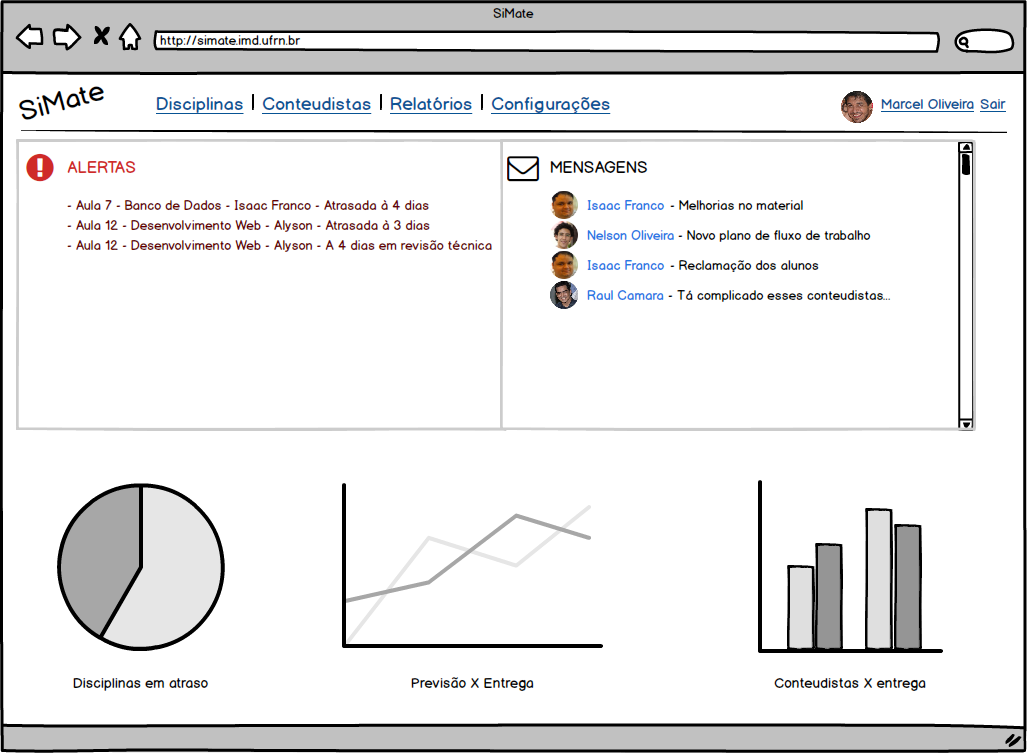
\includegraphics[width=15cm]{Wireframes/DashboardAdmin.png}
    \captionof{figure}{Tela Inicial do Administrador}
	\label{fig:wf_dashboard_admin}
\end{minipage} \\

Ainda na figura \hyperref[fig:wf_dashboard]{\ref{fig:wf_dashboard}}, a seção \textit{Meus fluxos de trabalho ativos} é colocada para encurtar o caminho que o usuário precisa percorrer até ter acesso às suas atividades. Através dessa técnica, é possível aumentar a percepção e reduzir o tempo necessário para acesso ao conteúdo principal do sistema.

Dado que o usuário administrador possui perfil de gestor, o espaço restante da tela inicial na figura \hyperref[fig:wf_dashboard_admin]{\ref{fig:wf_dashboard_admin}} é preenchido com gráficos expositivos das métricas do sistema.

Na tela seguinte (Figura \hyperref[fig:wf_offers_list]{\ref{fig:wf_offers_list}}), temos a representação da listagem de ofertas de disciplinas num quadro que busca destacar o estado de entrega e finalização dos materiais. A disposição de indicadores para cada estado possível do material se justifica no interesse do sistema em comunicar a completude das informações da oferta de forma eficiente.

\vspace{5mm}
\begin{minipage}[c]{\textwidth}
    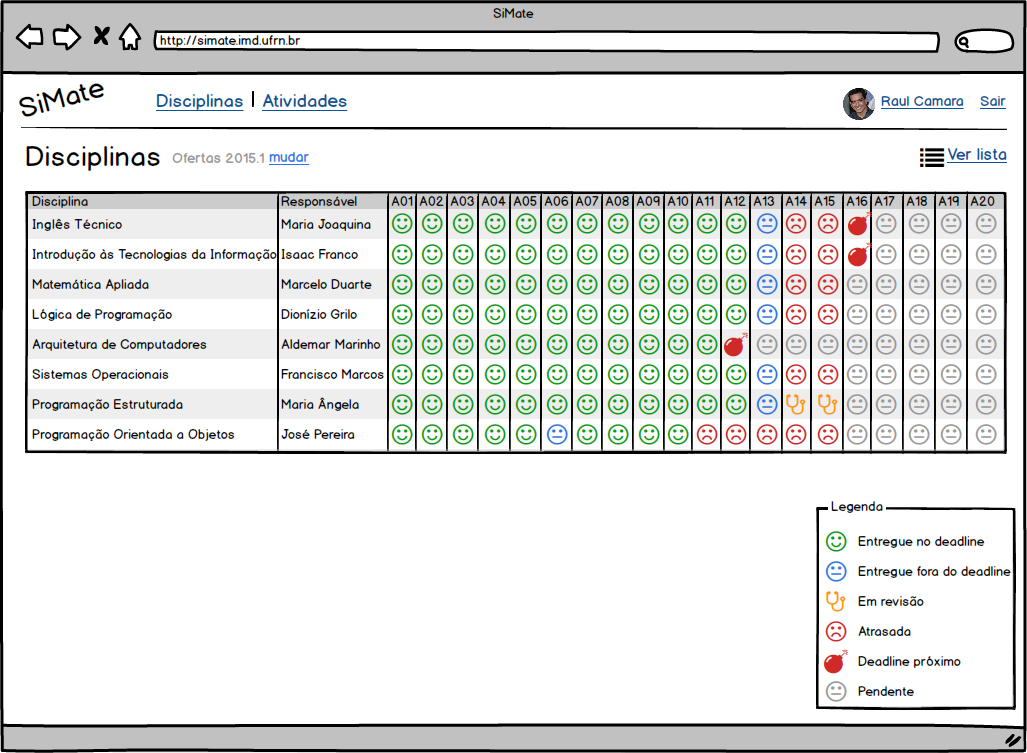
\includegraphics[width=15cm]{Wireframes/GradeDisciplinas.png}
    \captionof{figure}{Tela de Listagem das Ofertas}
	\label{fig:wf_offers_list}
\end{minipage} \\

O \textit{wireframe} \hyperref[fig:wf_material]{\ref{fig:wf_material}} representa a visualização mais completa do procedimento de criação de material. Nesta tela, as versões do material são organizadas de maneira cronológica com determinação das partes envolvidas e discussões criadas para cada passo dado. Também temos, ao lado direito, o formulário que permite a interação do usuário com o processo, novas versões são reflexos da submissão de conteúdo através desse formulário.

\vspace{5mm}
\begin{minipage}[c]{\textwidth}
    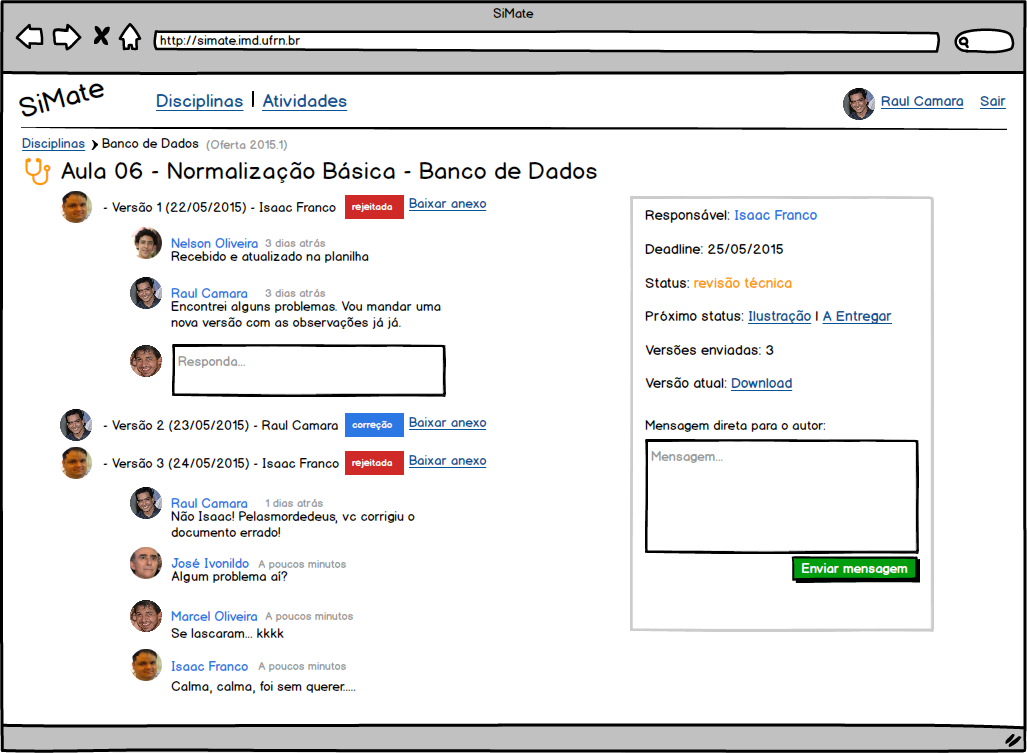
\includegraphics[width=15cm]{Wireframes/ArtefatoDetalhe.png}
    \captionof{figure}{Tela de Visualização do Material}
	\label{fig:wf_material}
\end{minipage} \\

As telas apresentadas nessa seção foram desenhadas por parte dos idealizadores do projeto, no processo de desenvolvimento de software, estas definem a visão esperada das partes mais importantes do sistema que se quer desenvolver na perspectiva do cliente, o que configuram aspectos de direcionamento e validação no processo de elicitação e detalhamento dos requisitos.

\section{Arquitetura}

O sistema Gema foi estruturado utilizando a arquitetura de desenvolvimento do setor de desenvolvimento do Instituto Metrópole Digital e suas versões foram gerenciadas utilizando uma ferramenta de controle de versão usada e testada nas dependências da instituição. A seguir iremos descrever mais profundamente como essas práticas foram realizadas.

\subsection{Framework IMDev}

O Framework IMDev define um conjunto de ferramentas elaboradas aos moldes das boas práticas de programação desenvolvidas e testadas ao longo do tempo pelo setor de desenvolvimento do IMD. A arquitetura desse conjunto de ferramentas é mantida buscando definir padrões de projeto para guiar a construção de novas aplicações dentro da instituição. Ao usar esse framework, a arquitetura do Gema mantém os padrões de projeto comuns às aplicações do instituto garantindo um ambiente conhecido para posterior manutenção e extensão por parte dos times de desenvolvimento.

A seguir descrevemos brevemente algumas das funcionalidades que fazem parte do pacote de interfaces extensíveis do Framework IMDev e que impactaram de forma mais profunda o desenvolvimento do sistema Gema.

\begin{enumerate}
	\item \textbf{Gerenciamento de usuários}: o pacote de funcionalidades para gerenciamento de usuários presente na arquitetura é de fácil utilização e permite a padronização estrutural de dados das aplicações da instituição;
	\item \textbf{Autenticação e controle de acessos}: utilizando o \textit{role-based access control (RBAC)}, em português \textit{controle de acesso baseado em papéis}, a arquitetura implementa entidades para gerenciamento de papéis e permissões que permitem restringir o acesso à funcionalidades com base nas autoridades de cada usuário;
	\item \textbf{Notificações}: sem a necessidade de implementação adicional, esse serviço propicia o envio de e-mails customizáveis;
	\item \textbf{Gerenciamento de arquivos}: mecanismos de upload e download foram incorporados à arquitetura e viabilizam o gerenciamento de arquivos com organização em estrutura de diretórios e banco de dados.
\end{enumerate}

\textbf{MVC} é um padrão arquitetural de software que divide a camada de apresentação da aplicação em três outras camadas interconectadas. A primeira é a View, camada que exibe os dados e interage com o usuário. A segunda é a Model, camada de manipulação e dados. E por fim temos a Controller, camada responsável por receber as requisições, usar a camada Model para obter os dados e fazer as validações necessárias para responder o usuário utilizando a View. 

Na figura abaixo é possível visualizar a arquitetura geral da aplicação no escopo das funcionalidades da oferta lado a lado com a estrutura do Framework IMDev.

\begin{figure}[H]
\centering
     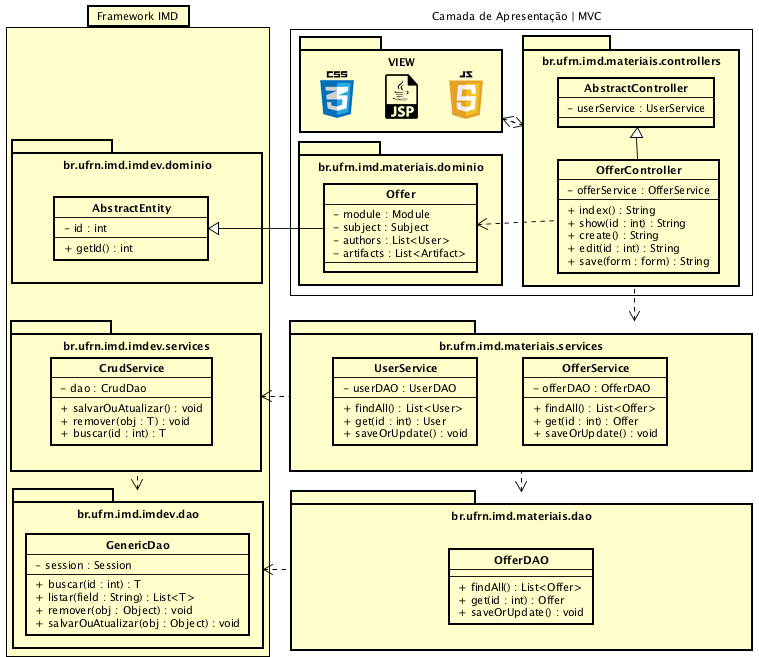
\includegraphics[width=1.0\textwidth]{Images/arq.png}
      \caption{Arquitetura do Gema em Função da Funcionalidade da Oferta}
       \label{fig:arq}
\end{figure}

A figura \hyperref[fig:arq]{\ref{fig:arq}} demonstra como cada camada da aplicação segue o padrão estabelecido pelo Framework de desenvolvimento do IMD. Na arquitetura, a camada de serviço serve para oferecer as ações disponíveis para manipulação de dados, ações essas que são executadas na camada de acesso aos dados (dao), esta é a responsável pela interação com a base de dados.

\subsection{Código Fonte}\label{sourceCode}

O código fonte do projeto desenvolvido é mantido no gerenciador de repositórios GitLab. Essa ferramenta permite que desenvolvedores armazenem código em servidores próprios dava prévia instalação da plataforma. 

A escolha do GitLab foi feita para seguir o padrão instituído no setor de desenvolvimento do IMD, dessa maneira, o repositório do Gema está alocado juntamente com os outros sistemas desenvolvidos no instituto, permitindo o acesso dos demais membros e gerentes do setor.

Para gerenciar as versões dos projetos, o GitLab utiliza o Git, sistema de controle de versão distribuído que surgiu para facilitar o desenvolvimento em equipes. Em resumo, o Git permite o desenvolvimento descentralizado e a junção das partes desenvolvidas utilizando mecanismos eficientes de comparação e mesclagem de código.

No que se diz respeito ao acesso ao repositório do Gema para estudo ou contribuição, é necessário que o usuário busque a devida autorização juntamente com a Diretoria de TI do Instituto Metrópole Digital.

\section{Usando o Gema}

Nesta seção, aprenderemos a usar o sistema Gema. Começaremos apresentando os perfis de navegação para que, nas subseções seguintes, os fluxos de uso demonstrados possam ser melhor entendidos. 

\subsection{Perfis de Navegação}\label{nav_perfis}

A aplicação concede suas funcionalidades com base nas autoridades em posse do usuário autenticado, sabendo disso podemos separar as possibilidades de navegação em três perfis diferentes, estes perfis serão indicados através das barras de navegação contidas na figura abaixo e detalhados logo em seguida.

\begin{figure}[H]
\centering
     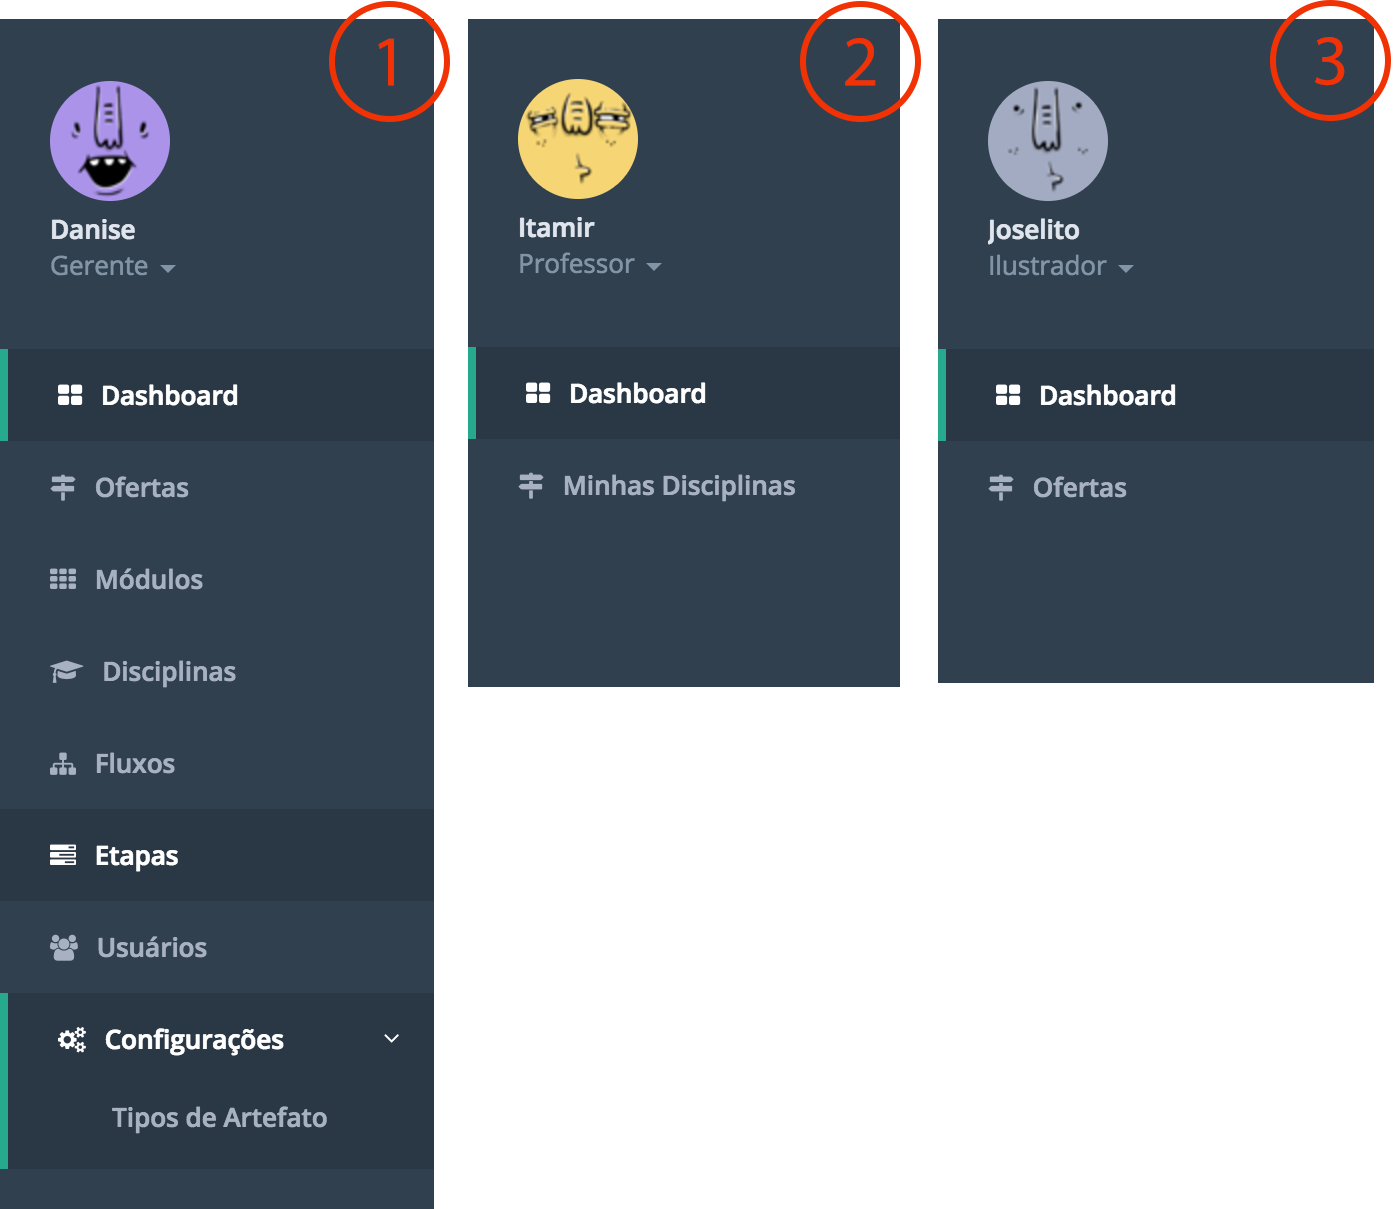
\includegraphics[width=1.0\textwidth]{Screens/Menu.png}
      \caption{Barras de Navegação}
       \label{fig:sc_nav_bar}
\end{figure}

\begin{enumerate}  
\item Gerência \\
	\textbf{Papel:} Gerência ou Gerenciamento \\
	\textbf{Descrição:} Este perfil é responsável por realizar a configuração e manutenção da base de dados para o funcionamento do sistema. Além disso, a gerência possui função de controle, validação e resolução de problemas gerais no fluxo de produção de material.
\item Autor \\
	\textbf{Papel:} Autor \\
	\textbf{Descrição:} Os autores são os usuários responsáveis pelas ofertas de disciplina, cabe a eles iniciar cada um dos fluxos de produção de  material, acompanhar o processo, fazer correções e, ao final, validar o que foi produzido.
\item Equipes de Produção Multimídia \\
	\textbf{Papéis:} Revisão Técnica, Transição Didática, Revisão LP, Revisão ABNT, Ilustração, Diagramação, Implementação Moodle, Tipografia e Vídeos. \\
	\textbf{Descrição:} As equipes de produção multimídia são encarregadas pelas etapas subsequentes a inicial do fluxo, executando tarefas com o objetivo de revisar, melhorar e complementar os materiais.
\end{enumerate}

%\subsection{Fluxos de Uso}\label{useFlows}

\subsection{Gerenciando o Gema}\label{managingTheSystem}

A prática de gerenciamento envolve a configuração dos modelos essenciais para funcionamento do fluxo de produção de material e a manutenção dos mesmos durante o período de vida útil do sistema. Nesta subseção, iremos aprender como configurar esses modelos e entender como eles estão conectados. O acesso aos itens listados fazem parte da navegação do perfil 1 da subseção \hyperref[nav_perfis]{\ref{nav_perfis}}.

Antes de começar, tomaremos um exemplo que será configurado passo a passo a cada item a seguir. Vamos supor a necessidade de ofertar a disciplina de Estrutura de Dados II no primeiro semestre de 2016 e de 2017. Definiremos também que essas duas ofertas possuirão 20 aulas e 3 provas cada e que o artefato de aula é representado por dois materiais, um texto base de aula e duas listas de questões. A prova contém somente o material que representa ela própria.

\subsubsection{Tipos de Artefato}\label{artifactTypes}

Artefato é o nome dado a uma agrupamento de materiais, tipos básicos de artefatos são aula e prova. Os tipos de artefatos configuram o conjunto de possibilidades a serem usados no sistema.

Ao usar o botão \textbf{Tipos de Artefatos} dentro do bloco \textbf{Configurações} na navegação, o usuário é direcionado à tela apresentada da figura \hyperref[fig:sc_artifact_types_list]{\ref{fig:sc_artifact_types_list}}.

\begin{figure}[H]
\centering
     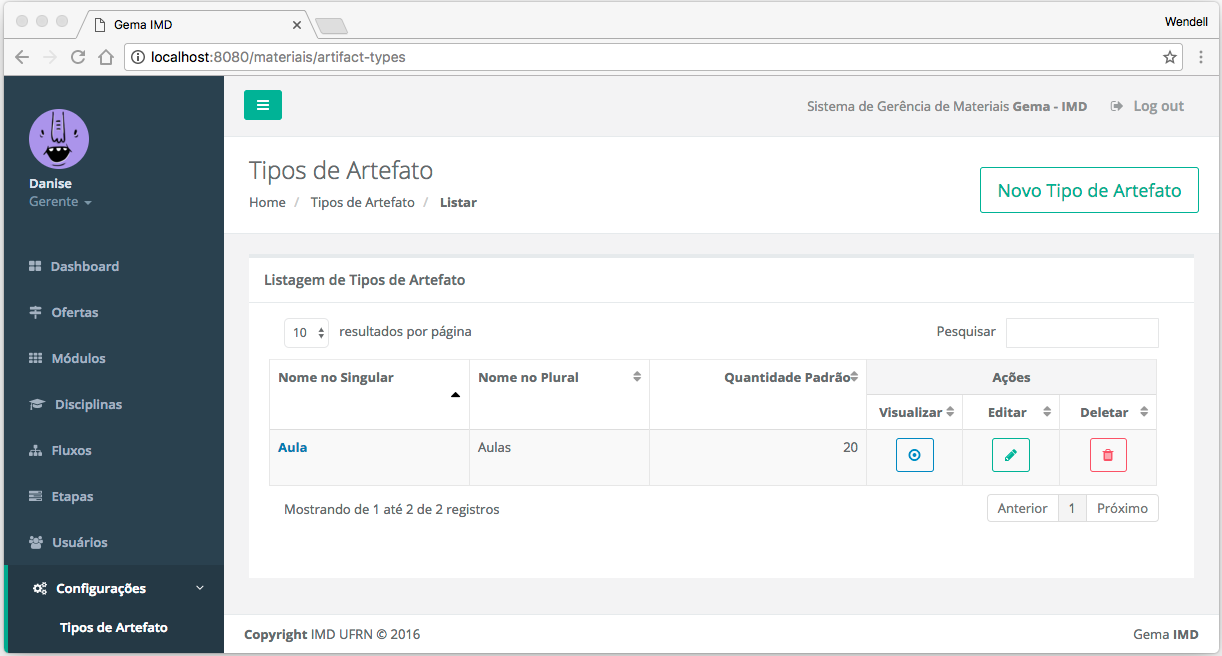
\includegraphics[width=1.0\textwidth]{Screens/ArtifactTypesList.png}
      \caption{Tela de Listagem de Tipos de Artefatos}
       \label{fig:sc_artifact_types_list}
\end{figure}

Seguindo o nosso exemplo, podemos visualizar que temos dois tipos de artefatos a serem configurados. A tela na figura \hyperref[fig:sc_artifact_types_list]{\ref{fig:sc_artifact_types_list}} mostra que o tipo pra aula já foi cadastrado, dessa maneira vamos cadastrar o tipo \textbf{Prova}.

Para efetuar a inserção de um novo tipo de artefato, deve-se usar o botão \textbf{Novo Tipo de Artefato} localizado no canto superior direito da tela de listagem. A resposta do sistema para essa ação segue na imagem abaixo.

\begin{figure}[H]
\centering
     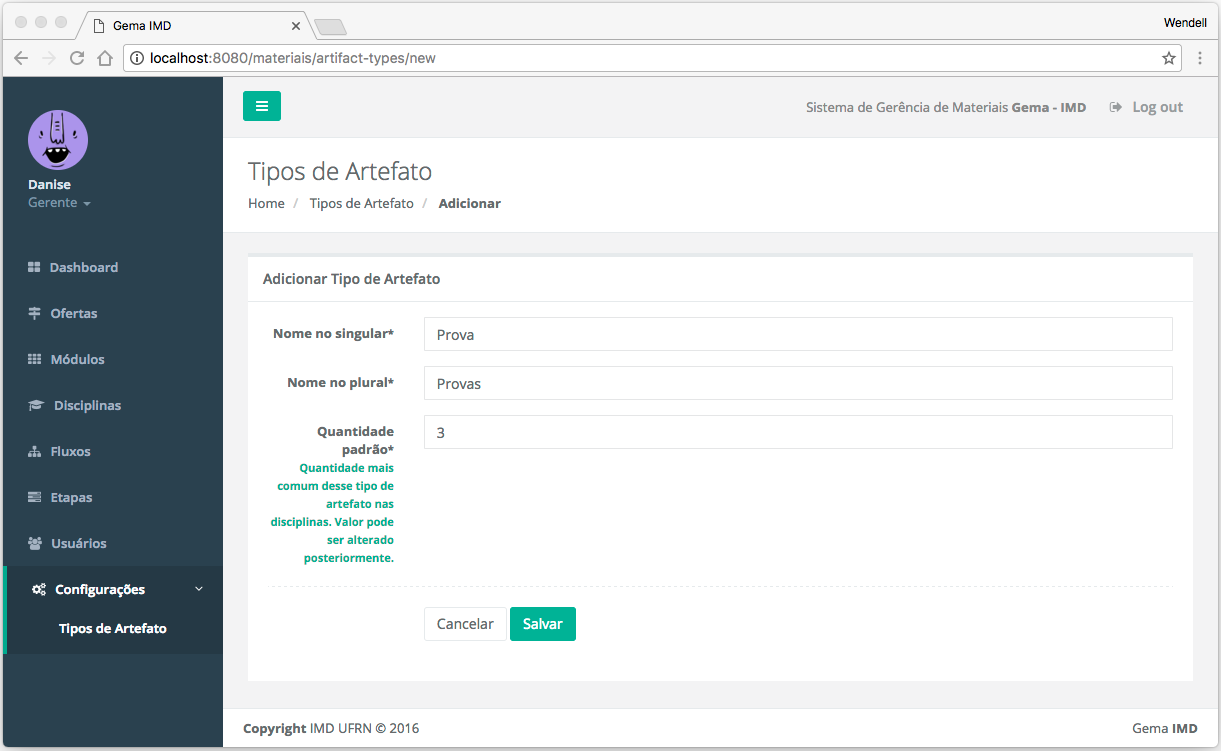
\includegraphics[width=1.0\textwidth]{Screens/ArtifactTypesForm.png}
      \caption{Formulário de Cadastro/Edição de Tipos de Artefatos}
       \label{fig:sc_artifact_types_form}
\end{figure}

O formulário da figura \hyperref[fig:sc_artifact_types_form]{\ref{fig:sc_artifact_types_form}} possui os campos \textit{Nome no singular} e \textit{Nome no plural} que representam o nome do tipo de artefato a serem usados como forma de categorizar os materiais das ofertas de disciplina. O campo \textit{Quantidade padrão} serve para que, ao criar uma disciplina, já se tenha um valor preenchido em cada tipo facilitando assim o uso de valores comumente usados.

Ao salvar o registro, os tipos \textbf{Aula} e \textbf{Prova} necessários para o exemplo estarão cadastrados. Seguimos com a configuração no próximo item.

\subsubsection{Disciplinas}

Os registros desse modelo no sistema representam o conjunto de disciplinas que podem ser ofertados no sistema e que possuem materiais a serem elaborados.

Ao usar o botão \textbf{Disciplinas} na navegação, o usuário é direcionado à tela de listagem apresentada da figura abaixo.

\begin{figure}[H]
\centering
     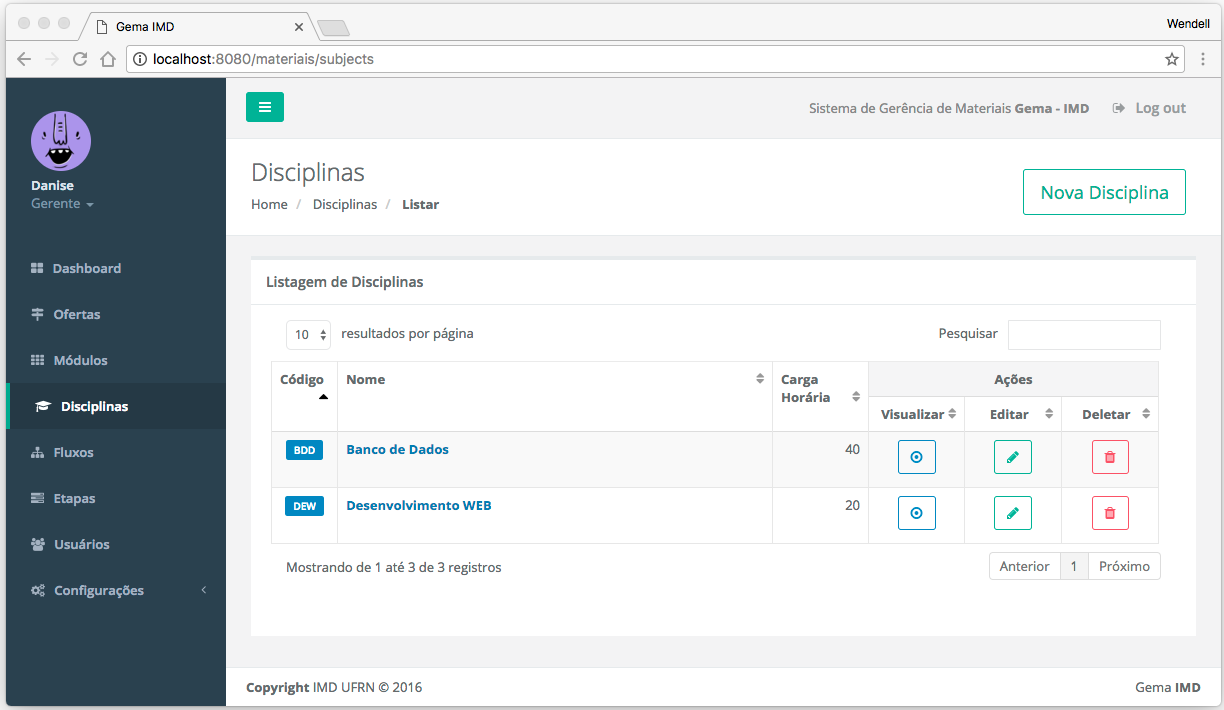
\includegraphics[width=1.0\textwidth]{Screens/SubjectsList.png}
      \caption{Tela de Listagem de Disciplinas}
       \label{fig:scSubjectsList}
\end{figure}

Para efetuar a inserção de uma nova disciplina, deve-se clicar no botão \textbf{Nova Disciplina} localizada no canto superior direito da tela de listagem. A resposta do sistema para essa ação segue na imagem abaixo.

\begin{figure}[H]
\centering
     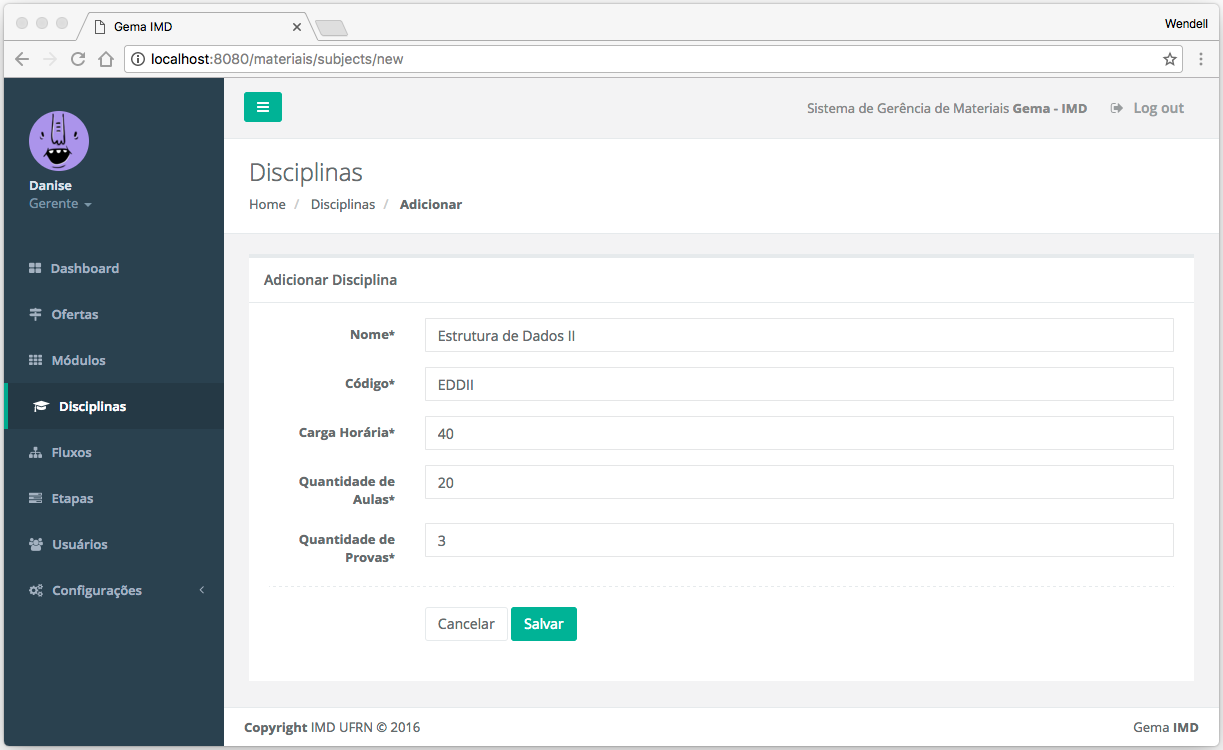
\includegraphics[width=1.0\textwidth]{Screens/SubjectsForm.png}
      \caption{Formulário de Cadastro/Edição de Disciplinas}
       \label{fig:scSubjectsForm}
\end{figure}

A identificação da disciplina é feita através dos campos \textit{Nome} e \textit{Código} do formulário da figura \hyperref[fig:scSubjectsForm]{\ref{fig:scSubjectsForm}}. O campo \textit{Carga Horária}, apesar de obrigatório, não infere em mudança de comportamento da aplicação, este serve para acentuar o nível de detalhamento na posterior visualização do registro. Os demais campos são referentes ao tipos de artefatos anteriormente inseridos no sistema.

Retomando o exemplo, o formulário da figura \hyperref[fig:scSubjectsForm]{\ref{fig:scSubjectsForm}} foi preenchido para cadastrar a disciplina de Estrutura de Dados II usando os tipos de artefatos previamente configurados a sinalizar as 20 aulas e 3 provas pretendidas.

\subsubsection{Módulos}\label{modules}

Definimos que a disciplina cadastrada deve ser ofertada em dois momentos: no primeiro semestre do ano 2016 e no primeiro semestre de 2017, além disso, iremos determinar que Estrutura de Dados II é uma disciplina avançada. Para que essas determinações sejam possíveis, será necessário configurar o sistema com dois módulos.

O primeiro passo pra essa configuração é usar usar o botão \textbf{Módulos} na navegação. Feito isso, o resultado segue na tela da figura \hyperref[fig:scModulesList]{\ref{fig:scModulesList}}.

\begin{figure}[H]
\centering
     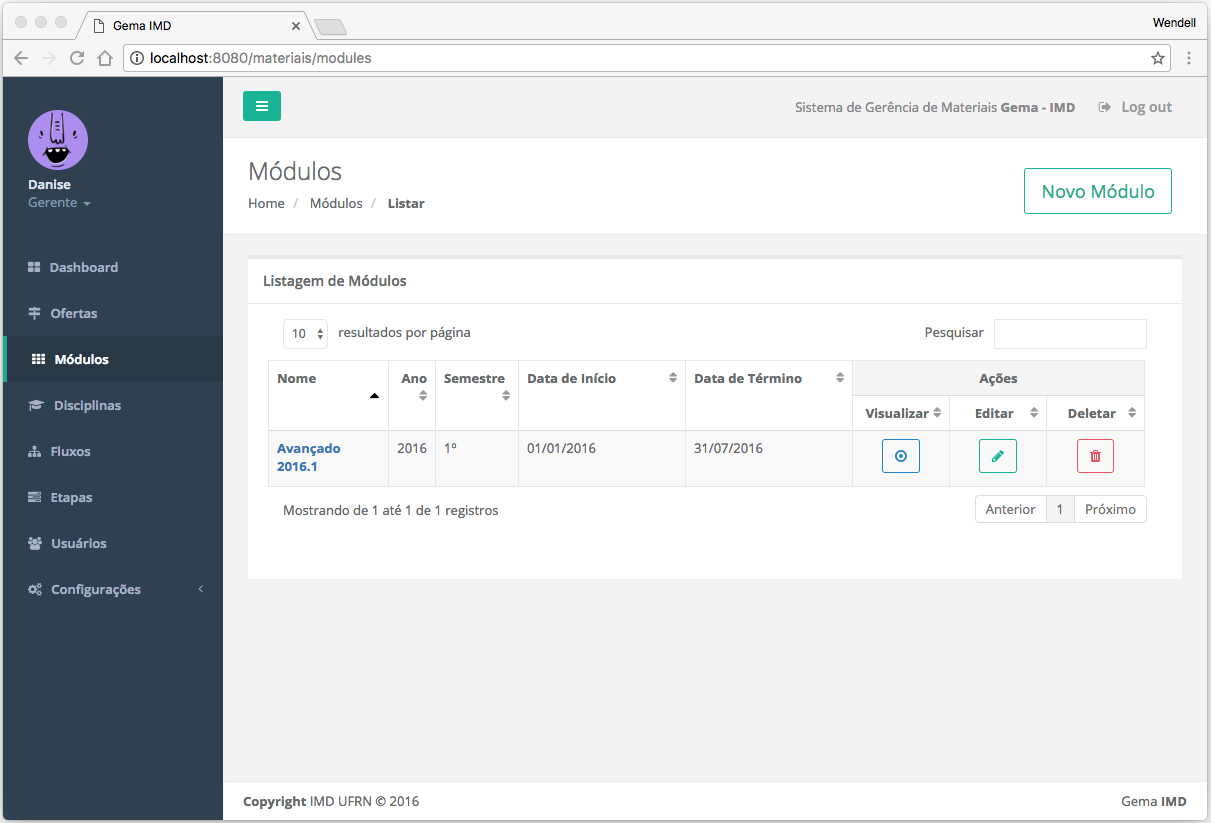
\includegraphics[width=1.0\textwidth]{Screens/ModulesList.png}
      \caption{Tela de Listagem de Módulos}
       \label{fig:scModulesList}
\end{figure}

Como é possível perceber na figura acima, o módulo Avançado 2016.1 já está cadastrado, cadastraremos então o Avançado 2017.1. 

Para efetuar a inserção de um novo módulo, deve-se clicar no botão \textbf{Novo Módulo} localizado no canto superior direito da tela de listagem. A resposta do sistema para essa ação está na imagem abaixo.

\begin{figure}[H]
\centering
     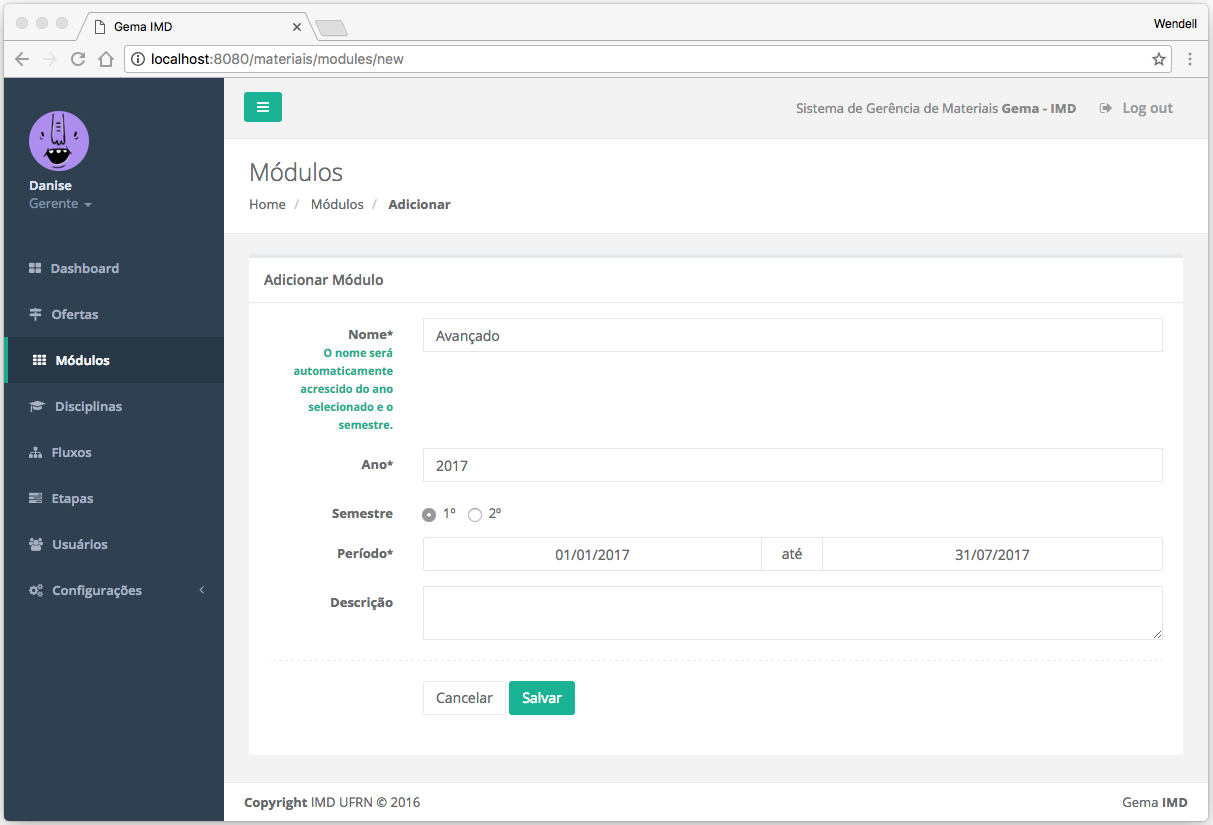
\includegraphics[width=1.0\textwidth]{Screens/ModulesForm.png}
      \caption{Formulário de Cadastro/Edição de Módulos}
       \label{fig:scModulesForm}
\end{figure}

O identificador da disciplina é formado pelo nome seguido do ano e semestre, dessa maneira, o módulo Avançado 2017.1 é o resultado do registro dos dados presentes no formulário da figura \hyperref[fig:scSubjectsForm]{\ref{fig:scSubjectsForm}}. 

Ao cadastrar um módulo, além dos dados de identificação é necessário definir o período em que ele ocorre. Esse intervalo deve ser determinado no campo de datas \textit{Período}.

\subsubsection{Etapas}

A configuração das etapas definem o conjunto de passos possíveis para serem usados na criação dos fluxos.

Ao usar o botão \textbf{Etapa} na navegação, o usuário é direcionado à tela de listagem apresentada da figura \hyperref[fig:scStepsList]{\ref{fig:scStepsList}}.

\begin{figure}[H]
\centering
     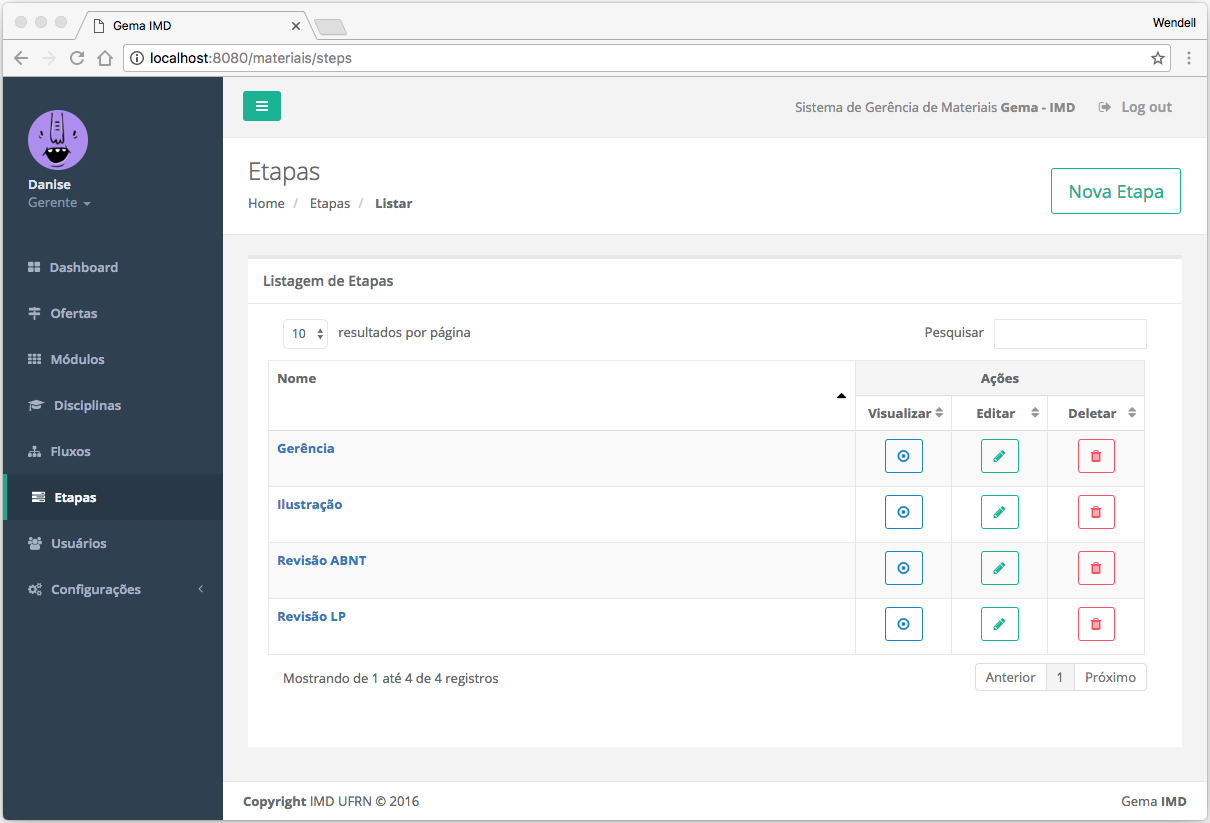
\includegraphics[width=1.0\textwidth]{Screens/StepsList.png}
      \caption{Tela de Listagem de Etapas}
       \label{fig:scStepsList}
\end{figure}

Para efetuar a inserção de uma nova etapa deve-se clicar no botão \textbf{Nova Etapa} localizado no canto superior direito da tela de listagem. A resposta do sistema para essa ação segue na imagem abaixo.

\begin{figure}[H]
\centering
     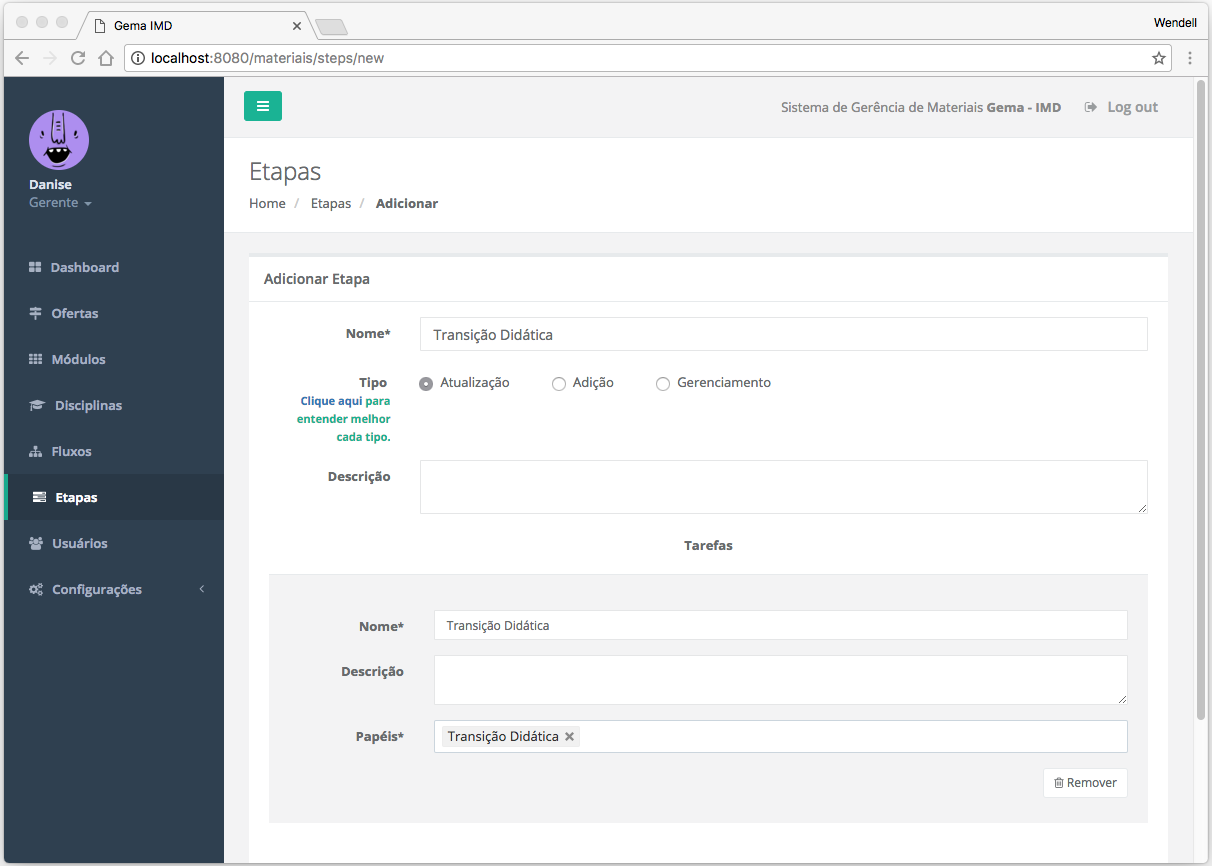
\includegraphics[width=1.0\textwidth]{Screens/StepsForm.png}
      \caption{Formulário de Cadastro/Edição de Etapas}
       \label{fig:csStepsForm}
\end{figure}

No formulário da etapa (figura \hyperref[fig:csStepsForm]{\ref{fig:csStepsForm}}), o campo \textit{Nome} identifica textualmente o modelo e o \textit{Tipo} pode determinar um dos seguintes comportamentos:

\begin{enumerate}  
\item Atualização: etapas desse tipo possuem uma só tarefa. Ao executá-las, o responsável deve baixar a versão atual do material, modificá-lo e submetê-lo atualizado. Após esse processo, a versão mais nova é a inserida pelo usuário.
\item Adição: pode possuir mais de uma tarefa, essa possibilidade se dá pelo fato dos responsáveis inserirem arquivos a serem adicionados à versão atual, i.e., na finalização da etapa, o material mais novo é a composição da versão atual somada com o submetido nas tarefas.
\item Gerenciamento: esta etapa é requisito para o funcionamento adequado do sistema. Ela deve estar associada ao papel de Gerência e será usada como alternativa para controle do fluxo de produção ou resolução de problemas.
\end{enumerate}

Os campos \textit{Nome} e \textit{Descrição} da tarefa irão determinar o que deve ser feito no momento do fluxo em que a etapa estiver vigente. Usuários com um dos papéis cadastrados no campo \textit{Papéis} serão apontados como responsáveis em resolver essa atividade.

Para cada equipe ou agrupamento de equipes que realize determinada função, é importante que uma etapa seja criada. Essa configuração permitirá que o sistema supra todos os fluxos reais no processo de produção de material.

\subsubsection{Fluxos}

O fluxo é o molde do processo a ser seguido para a criação de um material.

Relembrando nosso exemplo, por determinação, cada uma das 20 aulas possui três materiais, o texto base da aula e duas listas de questões. Para que esses materiais possam ser criados é necessário criar dois fluxos: o que molda o processo de criação do texto de aula e o que produz a lista de questões.

O primeiro passo para criar um fluxo é usar do botão \textbf{Fluxos} na navegação. Ao fazer isso, o usuário é direcionado à tela da figura a seguir.

\begin{figure}[H]
\centering
     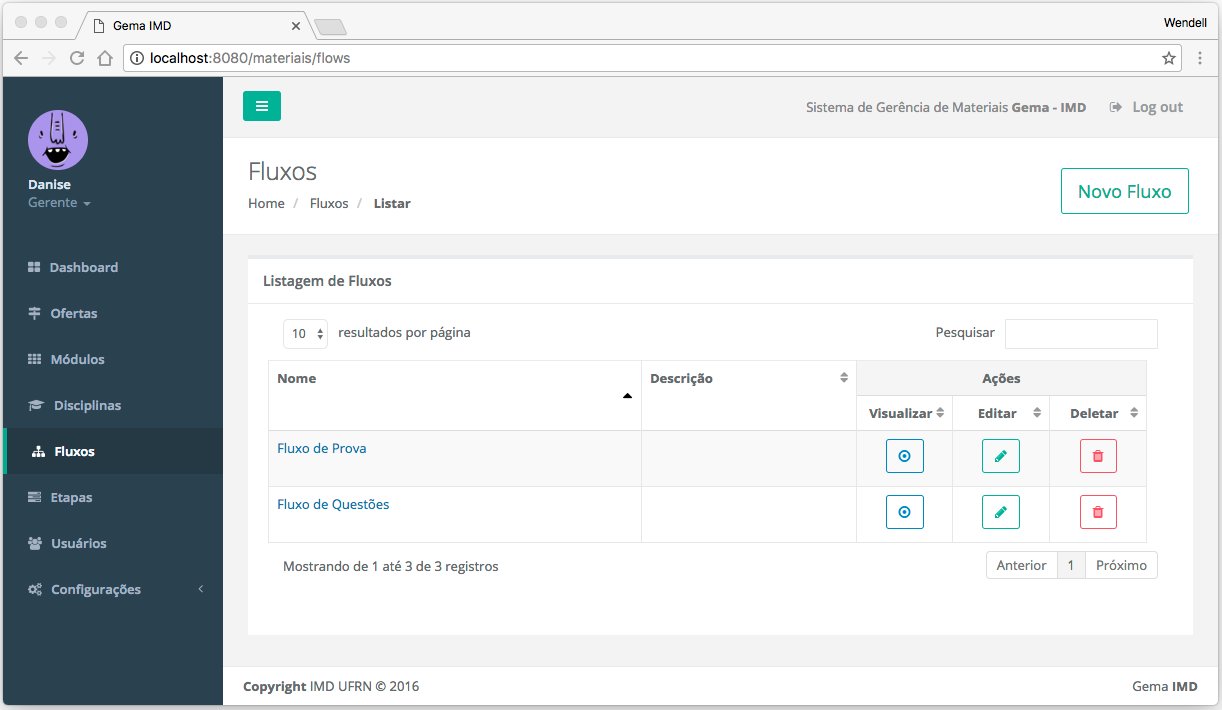
\includegraphics[width=1.0\textwidth]{Screens/FlowsList.png}
      \caption{Tela de Listagem de Fluxos}
       \label{fig:scFlowsList}
\end{figure}

Devemos clicar no botão \textbf{Novo Fluxo} localizada no canto superior direito da tela de listagem para efetuar o cadastro de um novo fluxo. A resposta do sistema para essa ação segue na imagem abaixo.

\begin{figure}[H]
\centering
     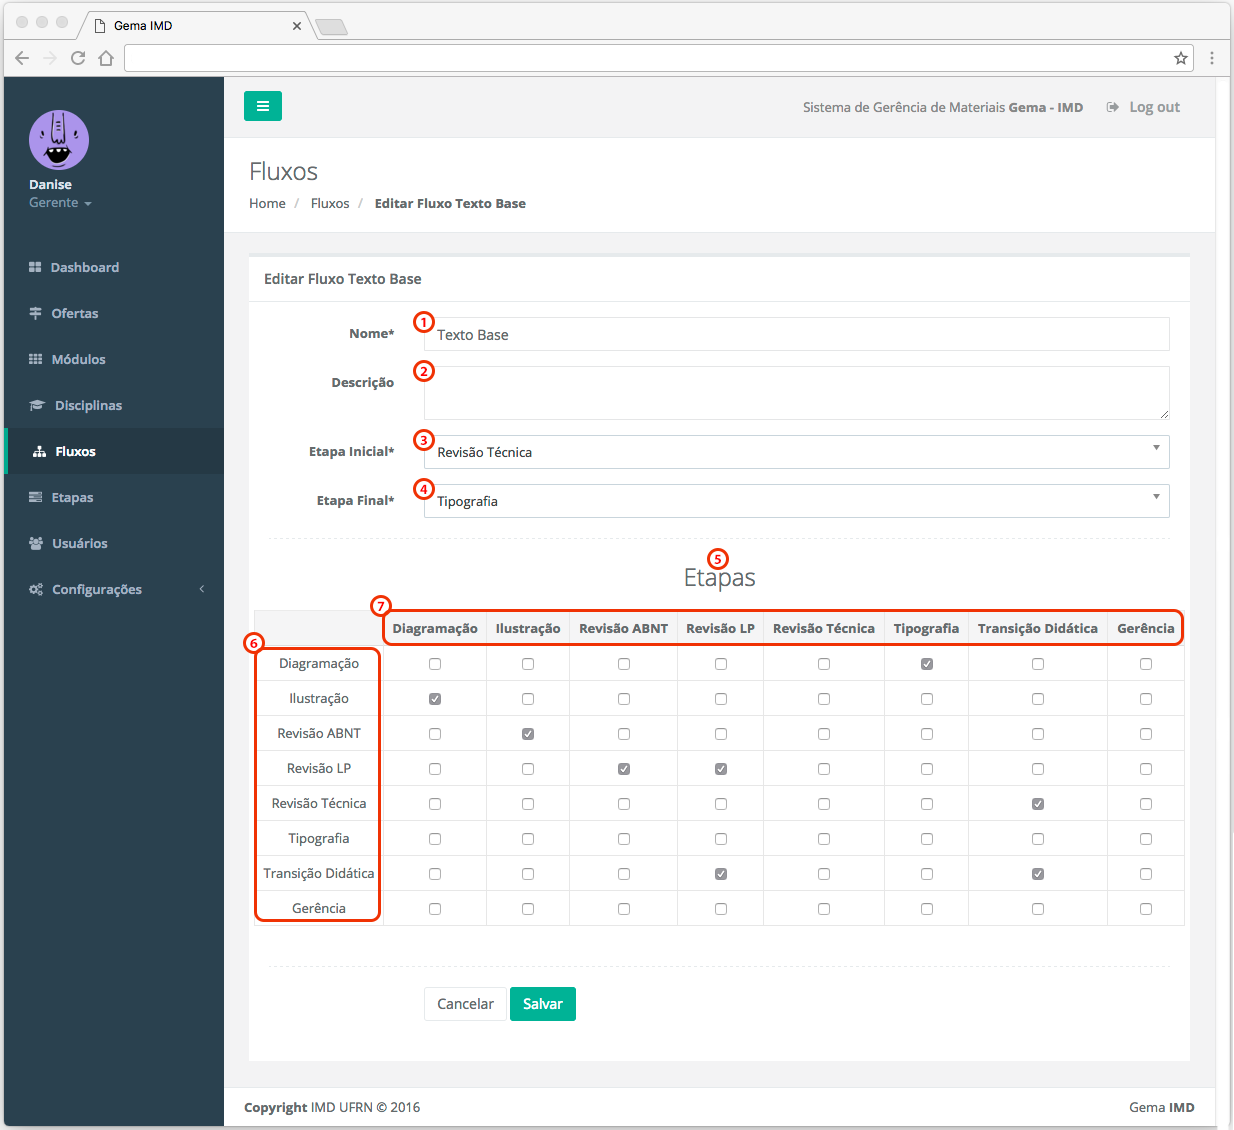
\includegraphics[width=1.0\textwidth]{Screens/FlowsForm.png}
      \caption{Formulário de Cadastro/Edição de Fluxos}
       \label{fig:scFlowsForm}
\end{figure}

Os marcadores no formulário da figura \hyperref[fig:scFlowsForm]{\ref{fig:scFlowsForm}} se caracterizam da seguinte forma:

\begin{enumerate}
	\item Nome que identifica o fluxo;
	\item Descrição para informações gerais;
	\item Indica a etapa que acontece logo após a submissão da versão inicial do material pelo professor, representa o início do fluxo;
	\item Indica o fim da produção do material e o início do processo de validação e finalização;
	\item Tabela que permite a conexão entre etapas. Ao relacionar duas etapas, configura-se que é possível enviar o material da etapa origem para a etapa destino no fluxo de produção;
	\item Conjunto de etapas possíveis para origem na conexão;
	\item Conjunto de etapas possíveis para destino da conexão;
\end{enumerate}

Os dados preenchidos no formulário da figura \hyperref[fig:scFlowsForm]{\ref{fig:scFlowsForm}} representam o fluxo para texto base de aula que será usado no nosso exemplo.

\subsubsection{Ofertas}

Oferta é a execução de uma disciplinas num determinado período. Toda oferta está na responsabilidade de um ou mais autores cuja função é submeter o material inicial dos artefatos (aulas, provas, etc.) para que o fluxo de  produção aconteça.

As configurações feitas até o presente momento determinam a base inicial necessária para que se possa ofertar a disciplina de Estrutura de Dados II durante os primeiros semestres de 2016 e 2017. Ao configurar essa oferta, estaremos dando o último passo para o início da execução dos fluxos de produção dos materiais.

Para fazer um novo registro, devemos usar o botão \textbf{Ofertas} na navegação e, em seguida, o botão \textbf{Nova Oferta} localizado no canto superior direito da tela de listagem, o resultado deve ser a tela representada na figura abaixo.

\begin{figure}[H]
\centering
     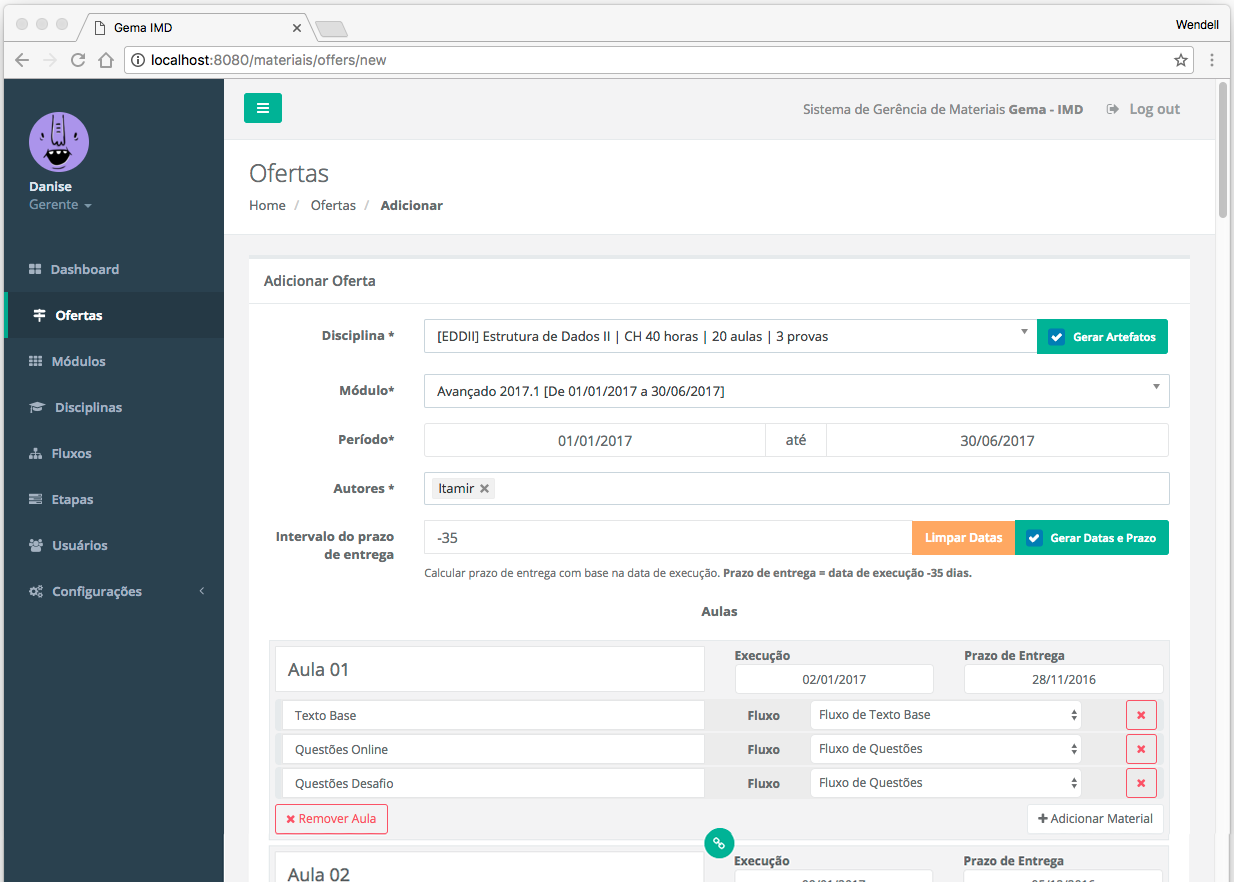
\includegraphics[width=1.0\textwidth]{Screens/OffersForm.png}
      \caption{Formulário de Cadastro/Edição de Ofertas (1/2)}
       \label{fig:scOfferForm}
\end{figure}

\begin{figure}[H]
\centering
     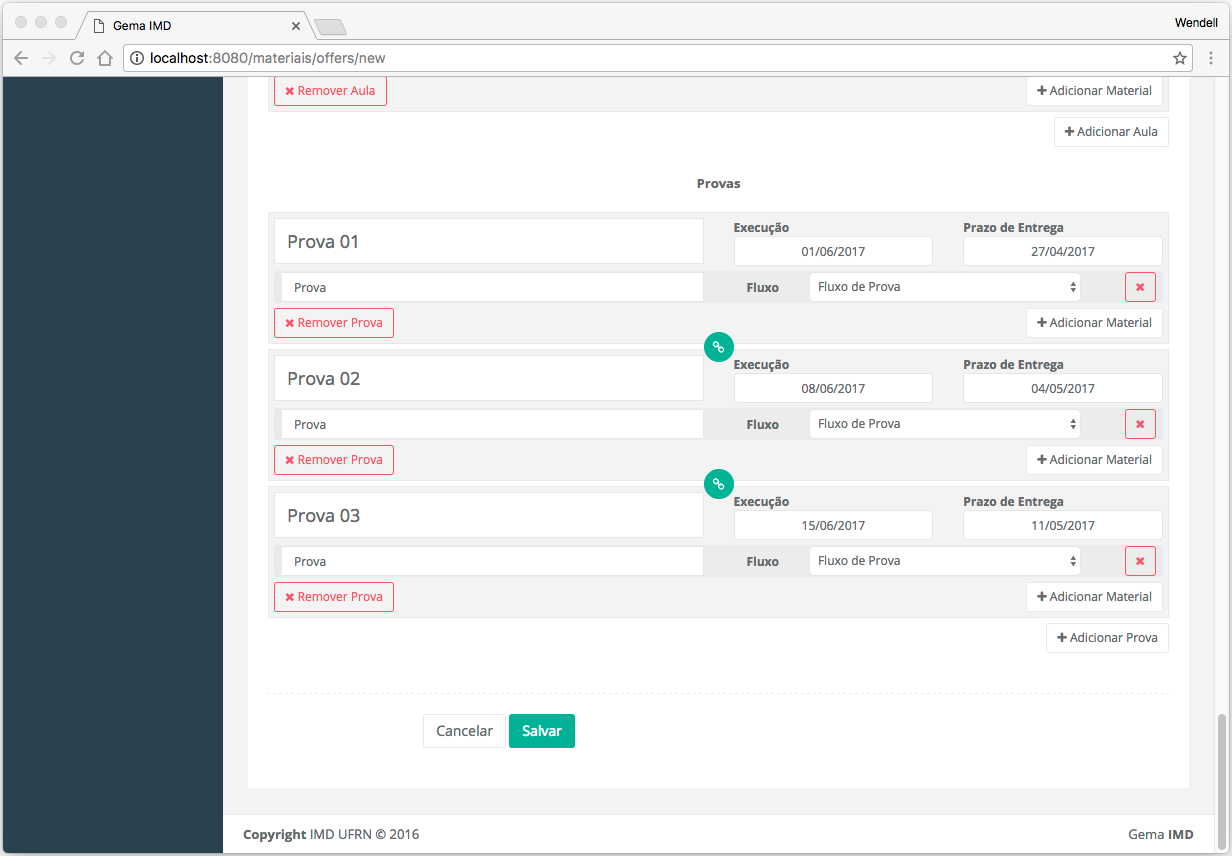
\includegraphics[width=1.0\textwidth]{Screens/OffersForm2.png}
      \caption{Formulário de Cadastro/Edição de Ofertas (2/2)}
       \label{fig:scOfferForm2}
\end{figure}

Na lista abaixo descrevemos os campos do formulário (figuras \hyperref[fig:scOfferForm]{\ref{fig:scOfferForm}} e \hyperref[fig:scOfferForm2]{\ref{fig:scOfferForm2}}).

\begin{itemize}
	\item \textit{Disciplina} e \textit{Módulo} são campos para seleção da disciplina e módulo que se quer utilizar. Seguindo o nosso exemplo,  selecionamos a disciplina Estrutura de Dados II e o módulo Avançado 2017.1.
	\item No campo \textit{Período} é possível definir as datas de início e término da oferta, essas datas são restringidas pelos limites do módulo escolhido.
	\item Os usuários responsáveis pela elaboração dos materiais devem ser escolhidos no campo \textit{Autores}.
	\item No campo \textit{Intervalo do prazo de entrega} um valor é selecionado para que a data dos campos \textit{Prazo de Entrega} sejam automaticamente calculados com base campos \textit{Execução} dos artefatos. Para limpar todas as datas do formulário, há o botão \textbf{Limpar Datas} e para desativar o gerador automático, há o marcador \textbf{Gerar Datas e Prazo}.
\end{itemize}

Após selecionar e preencher os campos listados acima, o formulário irá gerar os artefatos correspondentes as quantidades cadastradas na disciplina selecionada. No nosso caso, foram gerados 20 artefatos de aula e 3 de prova. A figura abaixo é um trecho da figura \hyperref[fig:scOfferForm]{\ref{fig:scOfferForm}} e será usada para detalhar os campos e ações na parte dos artefatos do formulário.

\begin{figure}[H]
\centering
     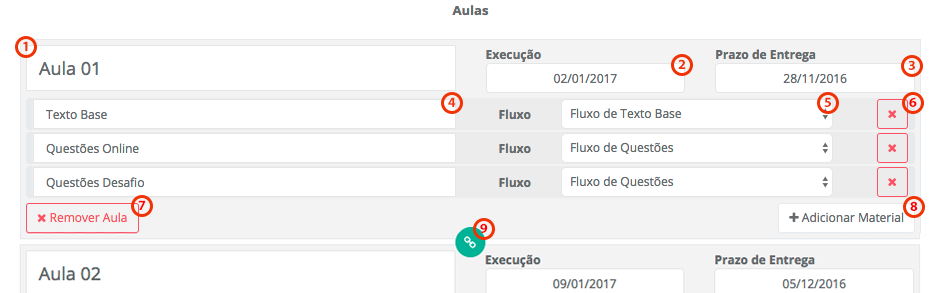
\includegraphics[width=1.0\textwidth]{Screens/ArtifactsForm.png}
      \caption{Parte da Seção de Artefatos do Formulário de Cadastro/Edição de Ofertas}
       \label{fig:scArtifactsForm}
\end{figure}

\begin{enumerate}
	\item Campo livre para escolha do nome do artefato. Como comportamento padrão, esse campo será automaticamente preenchido no formato <nome do artefato> <contador>. Sabendo disso, no nosso exemplo foram gerados 20 artefatos de aula nomeados Aula 01, Aula 02, Aula 03, ..., Aula 20 e três artefatos de prova nomeados Prova 01, Prova 02 e Prova 03.
	\item A execução define a data máxima para que o fluxo de produção de todos os materiais do referente artefato estejam finalizados.
	\item O prazo de entrega determina a data máxima para início dos fluxos de produção, ou seja, a data máxima para que o autor submeta a primeira versão de todos os materiais do referente artefato.
	\item Campo livre para escolha do nome do material. No nosso exemplo, determinamos que uma aula possuirá texto base de aula, lista de questões online e lista de questões desafio.
	\item Escolha do fluxo a ser usado para a criação do material.
	\item Botão para remoção do material.
	\item Botão para remoção do artefato.
	\item Botão para adicionar um novo material ao artefato.
	\item Botão para associar dois artefatos. Ao associar artefatos, automaticamente igualamos suas datas de execução e prazo de entrega.
\end{enumerate}

Salvo o registro da oferta, o sistema está apropriadamente configurado para que os fluxos de produção aconteçam. Na subseção seguinte iremos percorrer o processo de produção de um material.

\subsection{Produzindo Materiais Multimídia}

Feita a configuração inicial do sistema (ver subseção \hyperref[managingTheSystem]{\ref{managingTheSystem}} do corrente capítulo), é possível pôr em prática o processo de criação de materiais. Aqui utilizaremos o material Texto Base do artefato Aula 01 da oferta de disciplina Estrutura de Dados II - Avançado 2017.1 para demonstrar a execução do fluxo de produção.

Abaixo segue o diagrama do fluxo de produção de texto base que será realizado, estaremos descrevendo este processo após a figura.

\begin{figure}[H]
\centering
     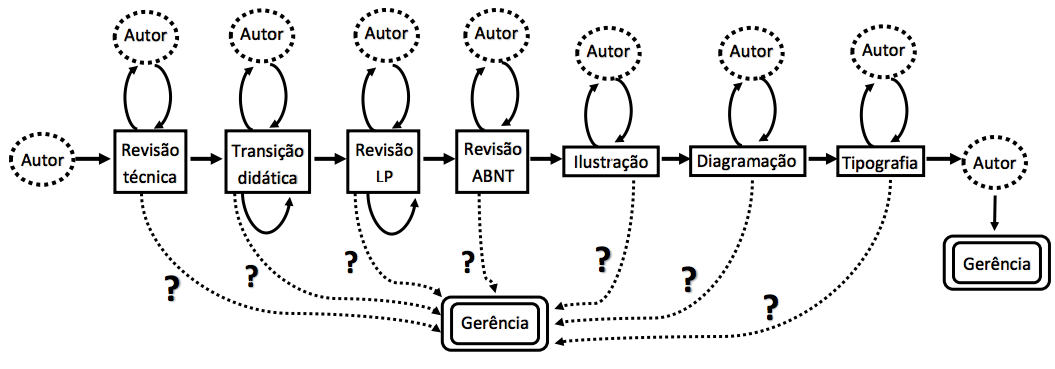
\includegraphics[width=1.0\textwidth]{Screens/Flow.png}
      \caption{Fluxo de Produção de Texto Base}
       \label{fig:flow}
\end{figure}

Por determinação, os fluxos começam com o envio do autor (representado pela elipse pontilhada na ponta esquerda do diagrama) e terminam com a validação do autor e finalização pela gerência (representados pela elipse e pelo retângulo no extremo direito). Entre esses dois extremos ocorrem as etapas intermediárias das equipes de produção multimídia (representadas pelos retângulos). 

Na parte superior do diagrama, a conexão bidirecional dos retângulos com os círculos do autor representam a possibilidade de enviar o material para correção. Já na parte inferior, a conexão com a gerência representa a possibilidade do envio do material para gerenciamento ou resolução de problemas não especificados.

\subsubsection{Iniciando o Fluxo de Produção}

Para iniciar o fluxo de produção do material escolhido no nosso exemplo, utilizaremos o perfil do autor (perfil de navegação 2 da subseção \hyperref[nav_perfis]{\ref{nav_perfis}}).

Após autenticado, o usuário autor será redirecionado a tela inicial de seu perfil, esta é demonstrada na figura abaixo.

\begin{figure}[H]
\centering
     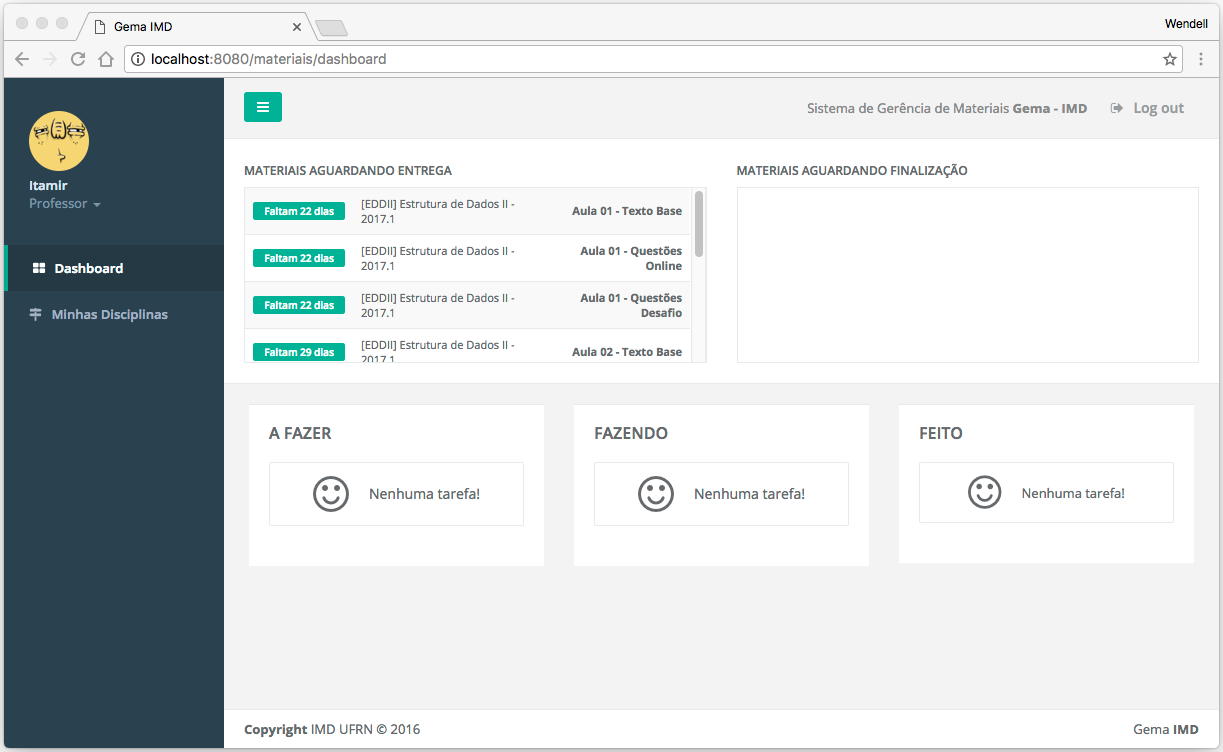
\includegraphics[width=1.0\textwidth]{Screens/DashboardAuthor.png}
      \caption{Tela Inicial do Professor}
       \label{fig:DashboardAuthor}
\end{figure}

É possível ver na figura acima a caixa intitulada \textbf{MATERIAIS AGUARDANDO ENTREGA}, esses itens são os materiais das aula cujo professor é responsável e estão aguardando a submissão da primeira versão para início do fluxo de produção.

Para continuar o exemplo, iremos selecionar o primeiro item da listagem que representa a Aula 01 - Texto Base da oferta [EDDII] Estrutura de Dados II - 2017.1. A resposta do sistema para essa ação está na figura a seguir. 

\begin{figure}[H]
\centering
     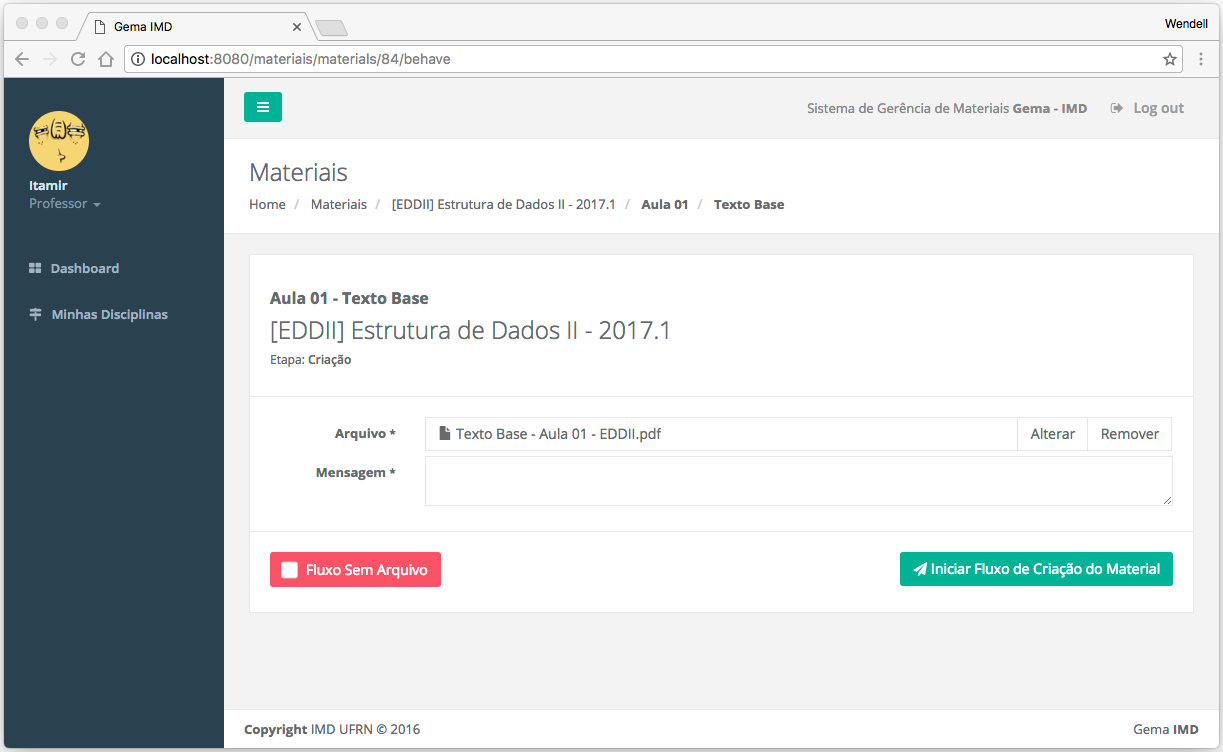
\includegraphics[width=1.0\textwidth]{Screens/StartMaterialFlow.png}
      \caption{Tela de Início do Fluxo de Material}
       \label{fig:StartMaterialFlow}
\end{figure}

Iniciar o fluxo do material escolhido significa submeter sua primeira versão, faremos isso inserindo um arquivo que representa o texto base da aula. Após selecionar o arquivo no formulário da figura \hyperref[fig:StartMaterialFlow]{\ref{fig:StartMaterialFlow}}, o botão \textbf{Iniciar Fluxo de Criação do Material} deve ser pressionado.

\textit{Obervação: caso haja a necessidade do autor em iniciar o fluxo de um material sem arquivo, o marcador \textbf{Fluxo Sem Arquivo} deve ser selecionado e, obrigatoriamente, uma mensagem descrevendo a situação deve ser inserida.}

\begin{figure}[H]
\centering
     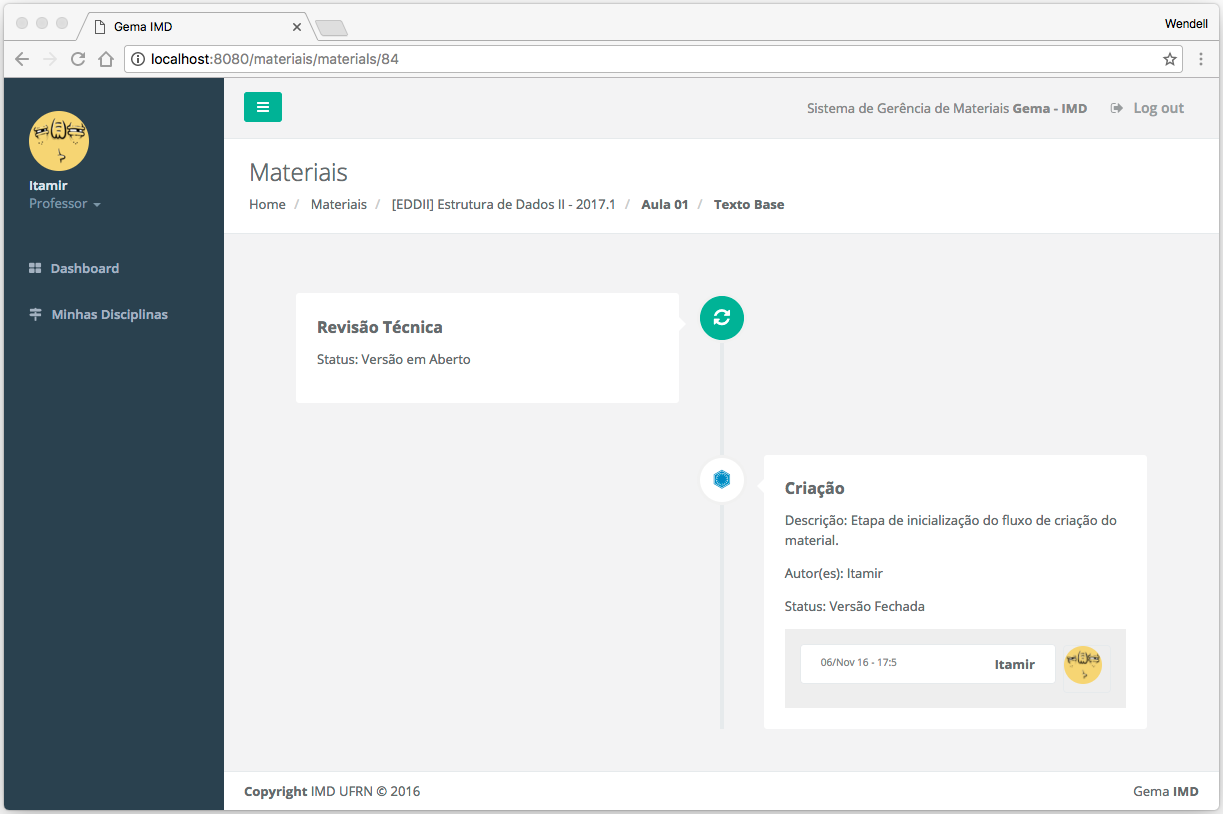
\includegraphics[width=1.0\textwidth]{Screens/MaterialTimeline.png}
      \caption{Tela de Linha do Tempo do Fluxo de Material}
       \label{fig:MaterialTimeline}
\end{figure}

A figura acima apresenta a tela de visualização do material e é resposta do sistema ao início do fluxo. Com o decorrer do processo, essa visualização será acrescentada de caixas descritivas pra cada etapa formando uma linha do tempo de produção do material.

Seguindo a visualização da linha do tempo explanada, após a etapa de criação, o material encontra-se com uma versão em aberto na responsabilidade da equipe de revisão técnica. A atuação dessa equipe de produção multimídia será explicada na próxima subseção. 

\subsubsection{Realizando Etapas do Fluxo de Produção}

Como determinado no fluxo de produção de texto base, a etapa Revisão Técnica é a que sucede a fase de início do fluxo, para realizá-la, utilizaremos o perfil de equipe de produção multimídia (perfil de navegação 3 da subseção \hyperref[nav_perfis]{\ref{nav_perfis}}).

Após autenticação, o usuário será redirecionado a sua tela inicial, esta está demonstrada na figura abaixo.

\begin{figure}[H]
\centering
     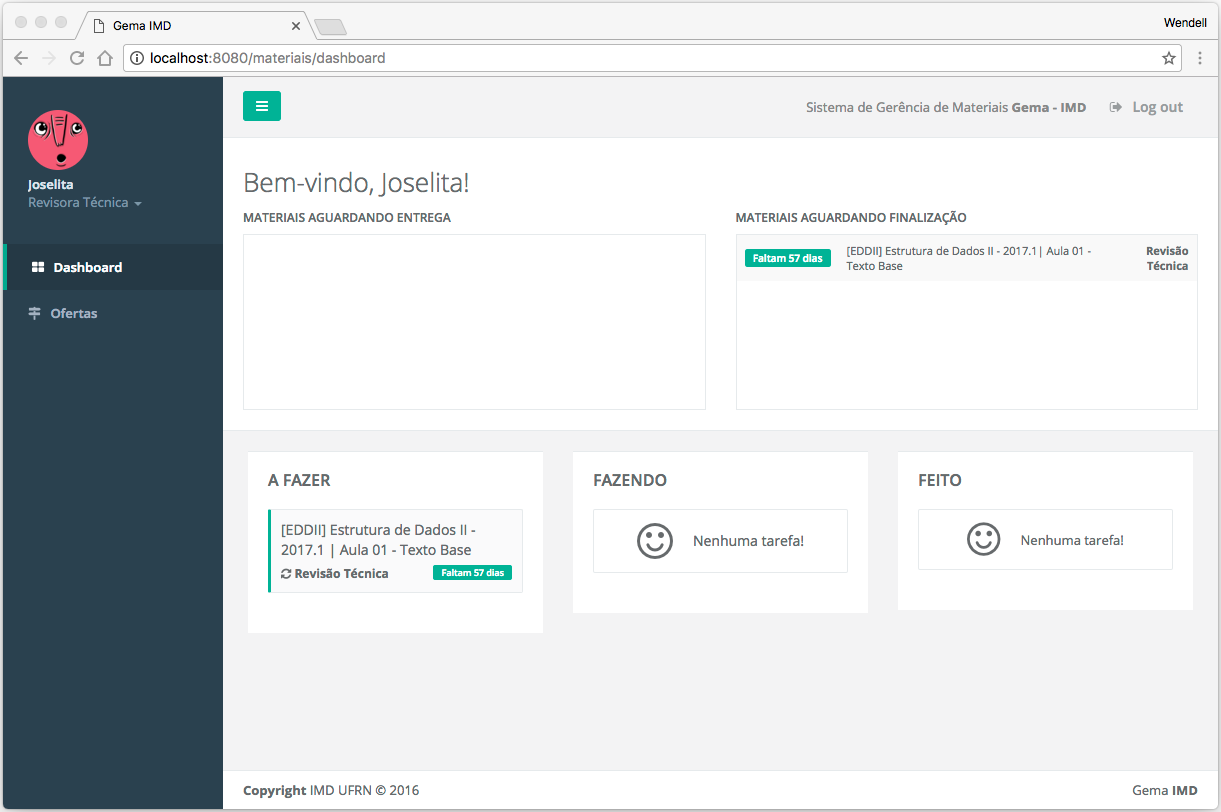
\includegraphics[width=1.0\textwidth]{Screens/DashboardProduction.png}
      \caption{Tela Inicial dos Membros das Equipes de Produção Multimídia}
       \label{fig:DashboardProduction}
\end{figure}

Na tela inicial do usuário com papel de Revisão Técnica é possível ver as atividades a espera de resolução (caixa intitulada \textbf{A FAZER}). Essas atividades são filtradas de acordo com a equipe da qual o usuário pertence. 

Ao selecionar o cartão do material de texto base da aula 01, seremos redirecionados à tela da figura abaixo.

\begin{figure}[H]
\centering
     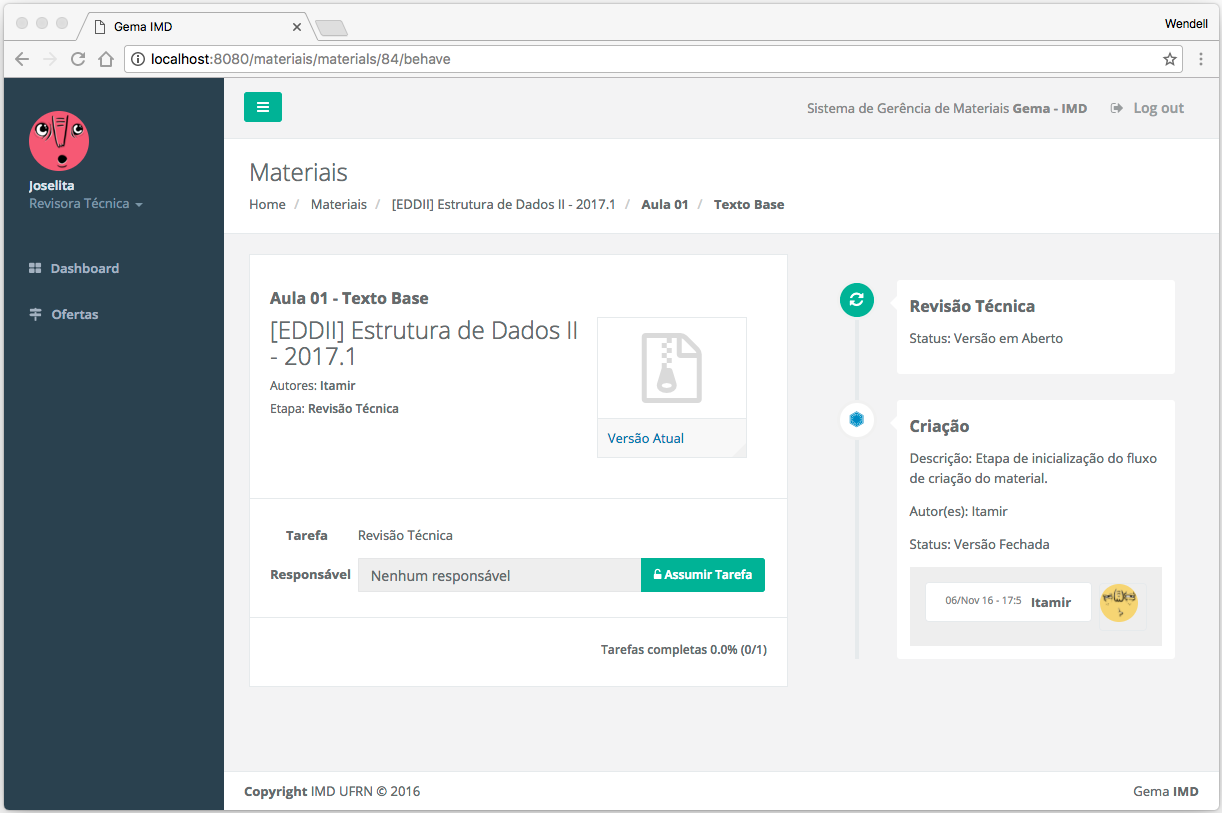
\includegraphics[width=1.0\textwidth]{Screens/BehaveMaterial.png}
      \caption{Tela do Passo 1 para Realização de Etapa}
       \label{fig:BehaveMaterial}
\end{figure}

Ao lado direito da tela da figura \hyperref[fig:BehaveMaterial]{\ref{fig:BehaveMaterial}} podemos perceber a linha do tempo do material e, ao lado esquerdo, o formulário para realização da etapa.

O primeiro passo a ser feito é usar o botão \textbf{Assumir Tarefa}, esta ação marcará o usuário logado como responsável e não permitirá que outros usuários resolvam a tarefa, além disso, o usuário será autorizado a resolvê-la de fato. 

\begin{figure}[H]
\centering
     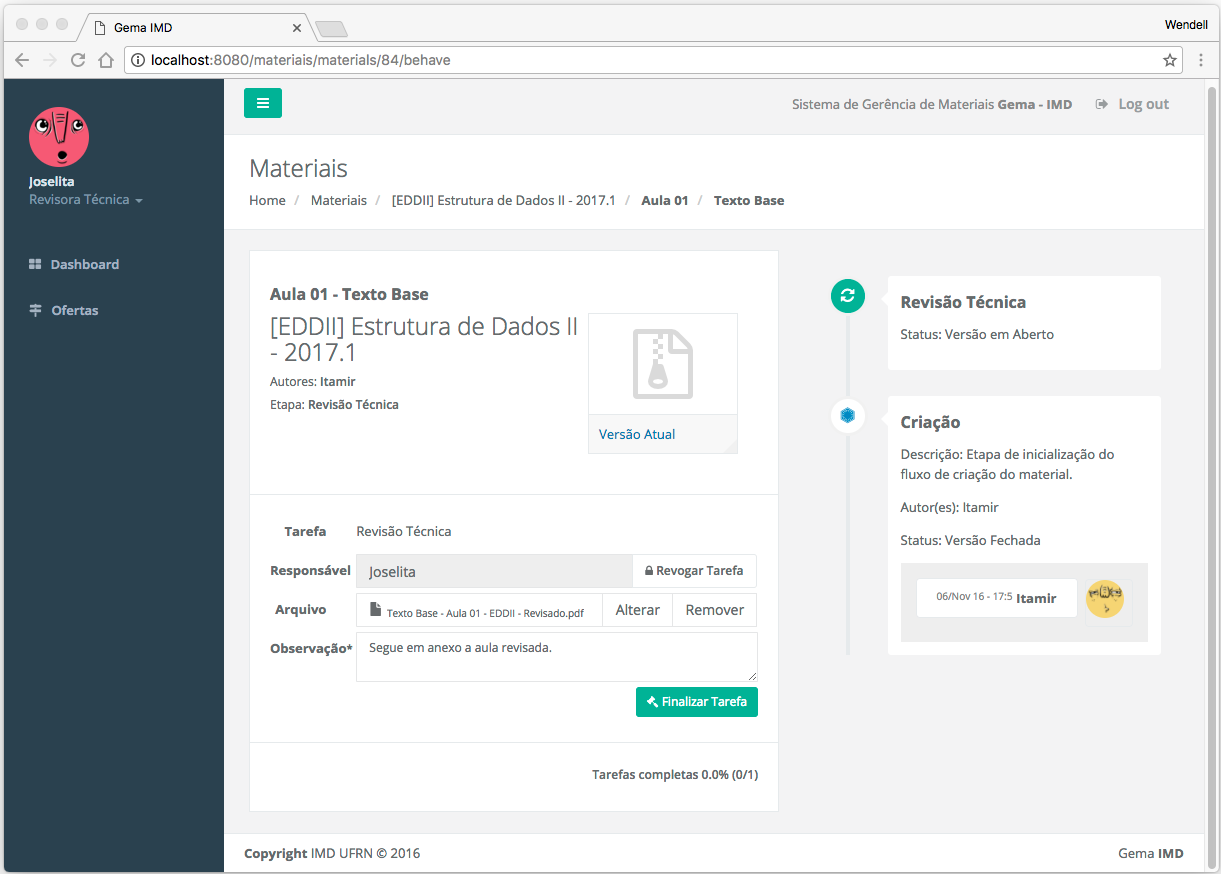
\includegraphics[width=1.0\textwidth]{Screens/BehaveMaterial2.png}
      \caption{Tela do Passo 2 para Realização de Etapa}
       \label{fig:BehaveMaterial2}
\end{figure}

Após assumir a tarefa, o formulário da tela acima torna-se disponível. Para finalizar a tarefa, o usuário deve submeter um arquivo ou fazer uma observação e usar o botão \textbf{Finalizar Tarefa}.

\begin{figure}[H]
\centering
     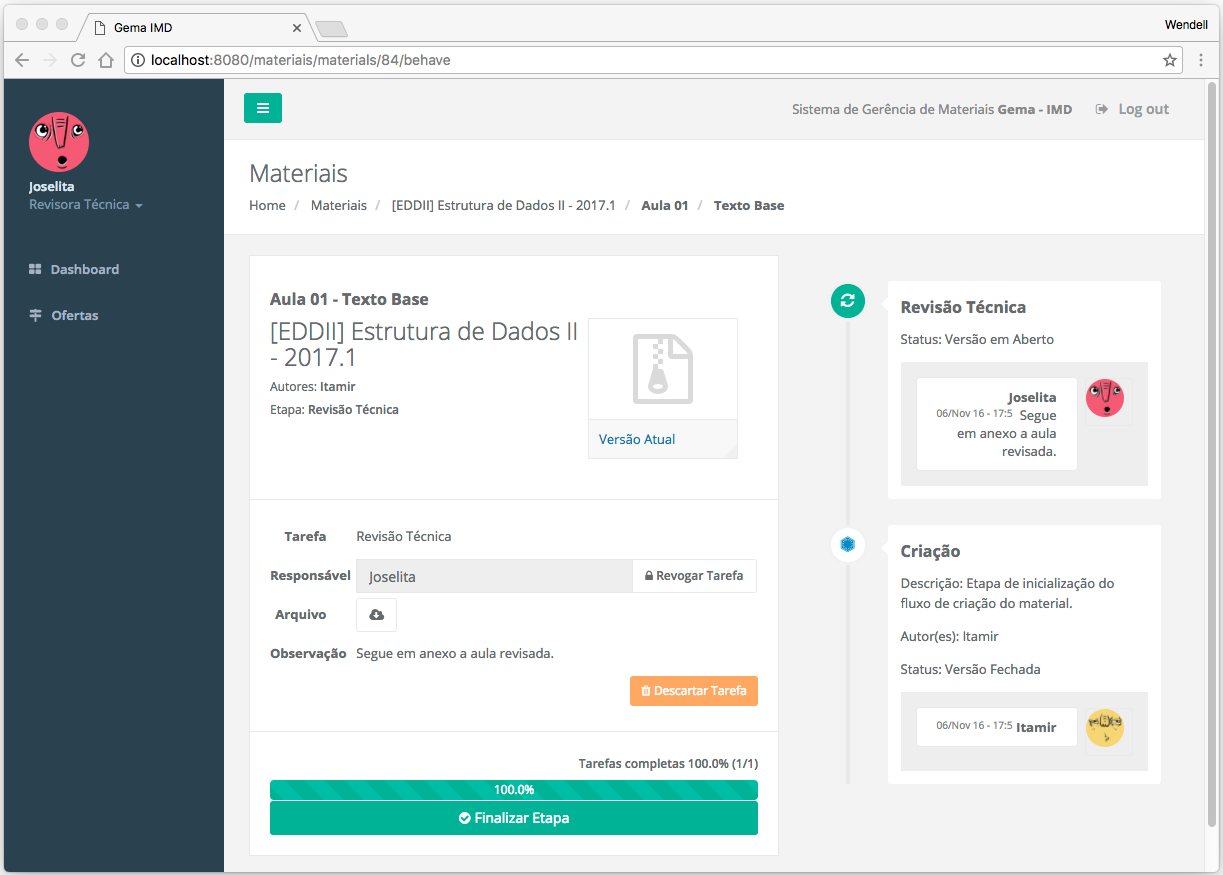
\includegraphics[width=1.0\textwidth]{Screens/BehaveMaterial3.png}
      \caption{Tela do Passo 3 para Realização de Etapa}
       \label{fig:BehaveMaterial3}
\end{figure}

No contexto do nosso exemplo, estamos realizando uma etapa de somente uma tarefa, sendo assim, logo após resolução da tarefa o sistema irá sinalizar que 100\% das tarefas estão completas e irá permitir a finalização da etapa. A tela da figura abaixo representa o resultado do uso do botão \textbf{Finalizar Etapa}.

\begin{figure}[H]
\centering
     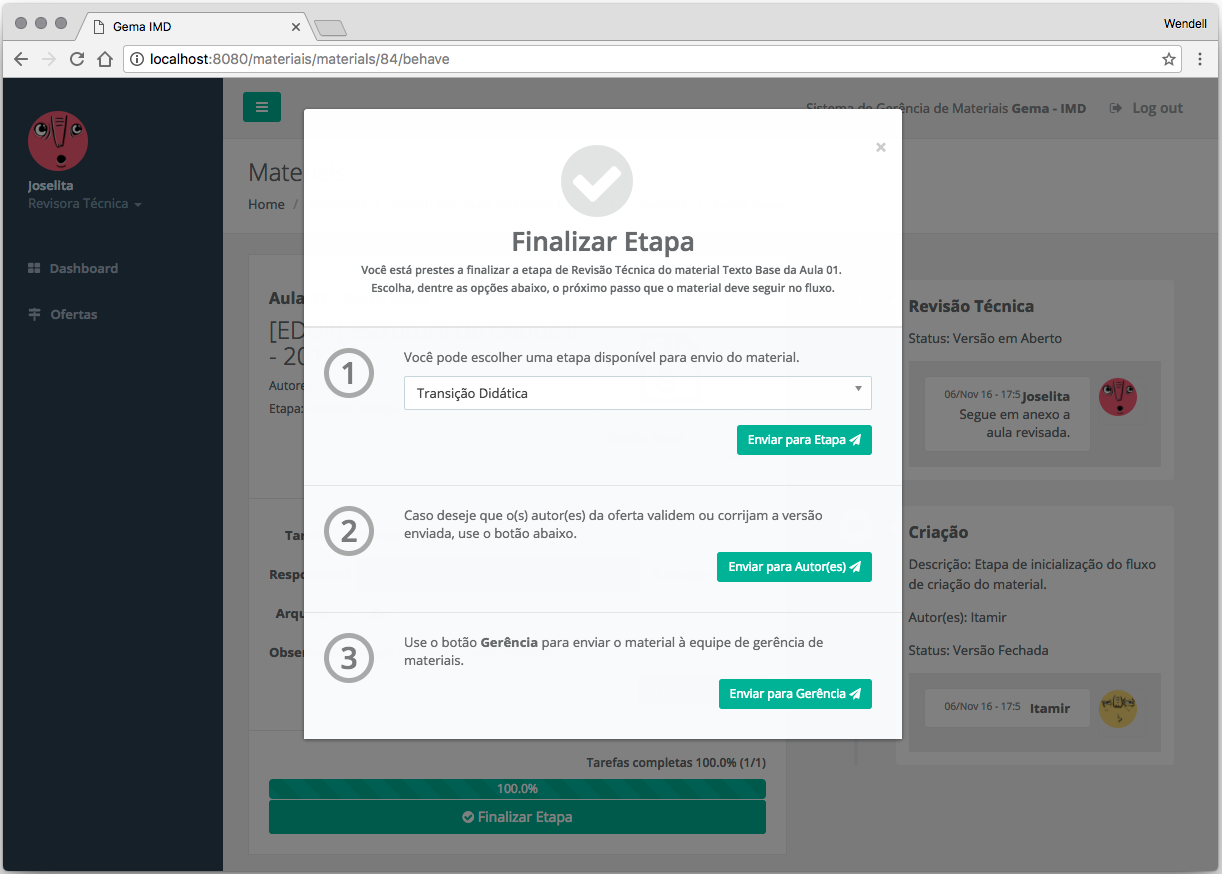
\includegraphics[width=1.0\textwidth]{Screens/BehaveMaterial4.png}
      \caption{Tela do Passo 4 para Realização de Etapa}
       \label{fig:BehaveMaterial4}
\end{figure}

Aqui é possível entender como o sistema apresenta as possibilidades de finalização de etapa representada no diagrama da figura \hyperref[fig:flow]{\ref{fig:flow}}. Na primeira opção teremos um campo de seleção onde as etapas possíveis do fluxo serão listadas. No segundo, há a possibilidade de enviar o material para correção por parte dos autores e, por último, há a opção do envio para a equipe de gerência.

A realização da etapa demonstrada nesta subseção representa o processo padrão para realização das etapas com exceção da etapa final. Na etapa final do fluxo de produção, o passo 4 é substituído pelo da tela na figura a seguir.

\begin{figure}[H]
\centering
     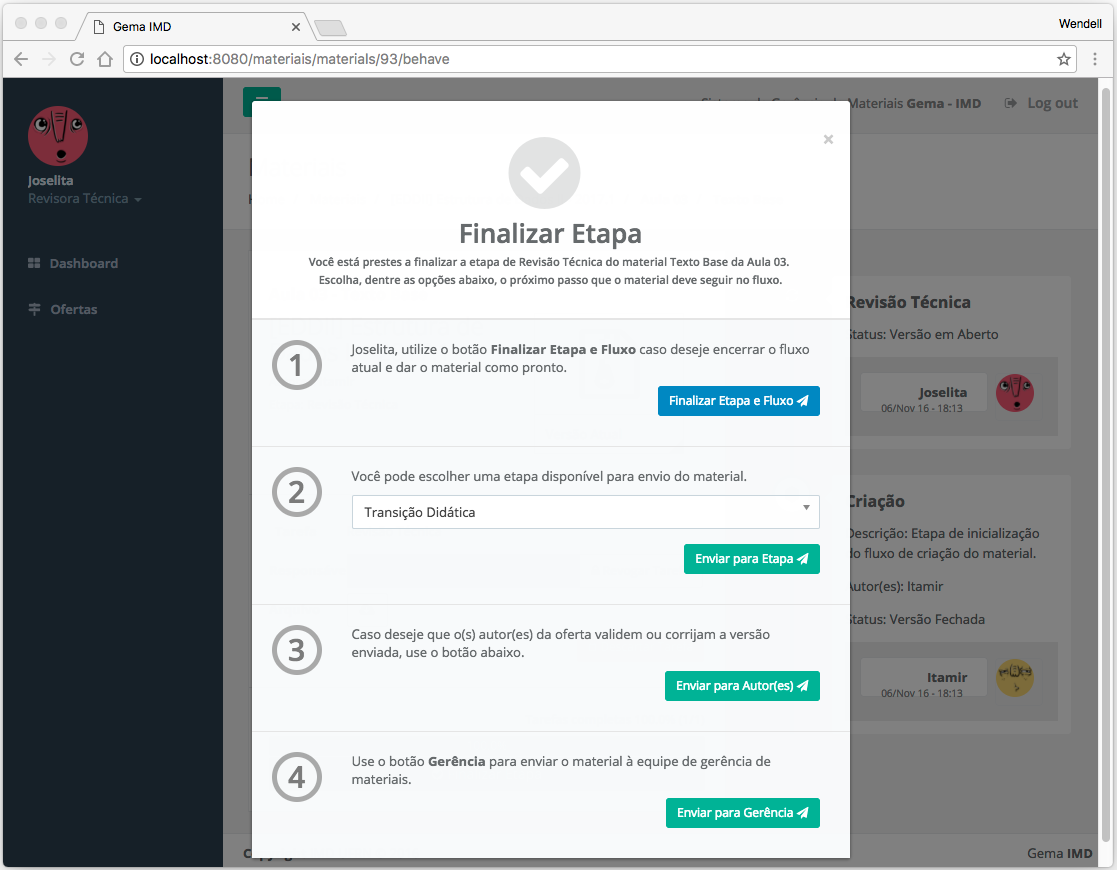
\includegraphics[width=1.0\textwidth]{Screens/BehaveMaterial5.png}
      \caption{Tela do Passo 4 para Realização de Etapa Final}
       \label{fig:BehaveMaterial5}
\end{figure} 

No momento do fluxo onde a etapa final estiver em realização, o usuário poderá, ao finalizá-la, iniciar também o processo de finalização do fluxo. Esse processo é demonstrado na subseção a seguir.

\subsubsection{Finalizando o Fluxo de Produção}

Após sinalizar a finalização do fluxo na etapa final, o material segue para a validação por parte dos autores da oferta. Nessa etapa, os autores devem analizar todo o conteúdo produzido e validá-lo.

Para demonstrar a validação do material, iremos usar o perfil de navegação do autor e, selecionaremos o botão \textbf{Minhas Disciplinas}.

\begin{figure}[H]
\centering
     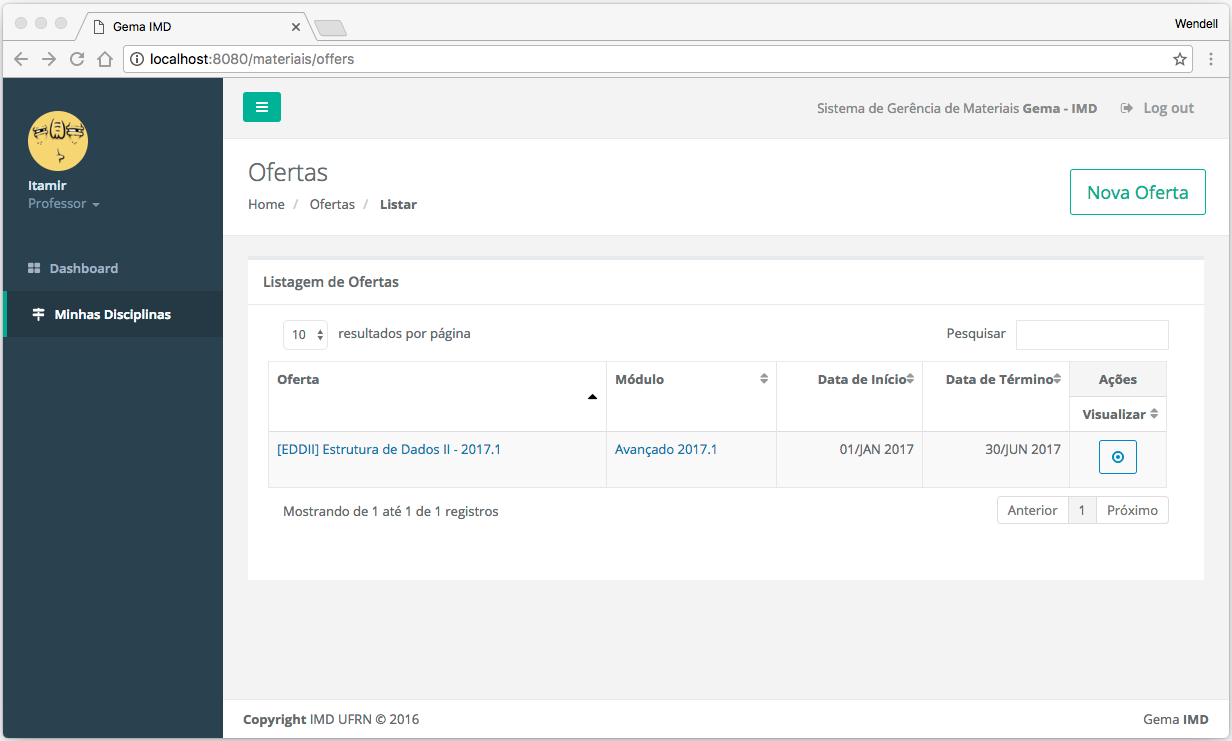
\includegraphics[width=1.0\textwidth]{Screens/OffersList.png}
      \caption{Tela de Listagem de Ofertas}
       \label{fig:OffersList}
\end{figure} 

Na tela de listagem de ofertas, devemos clicar no nome da oferta ou no botão de ação para visualizá-la. A figura a seguir mostra a tela de visualização da oferta.

\begin{figure}[H]
\centering
     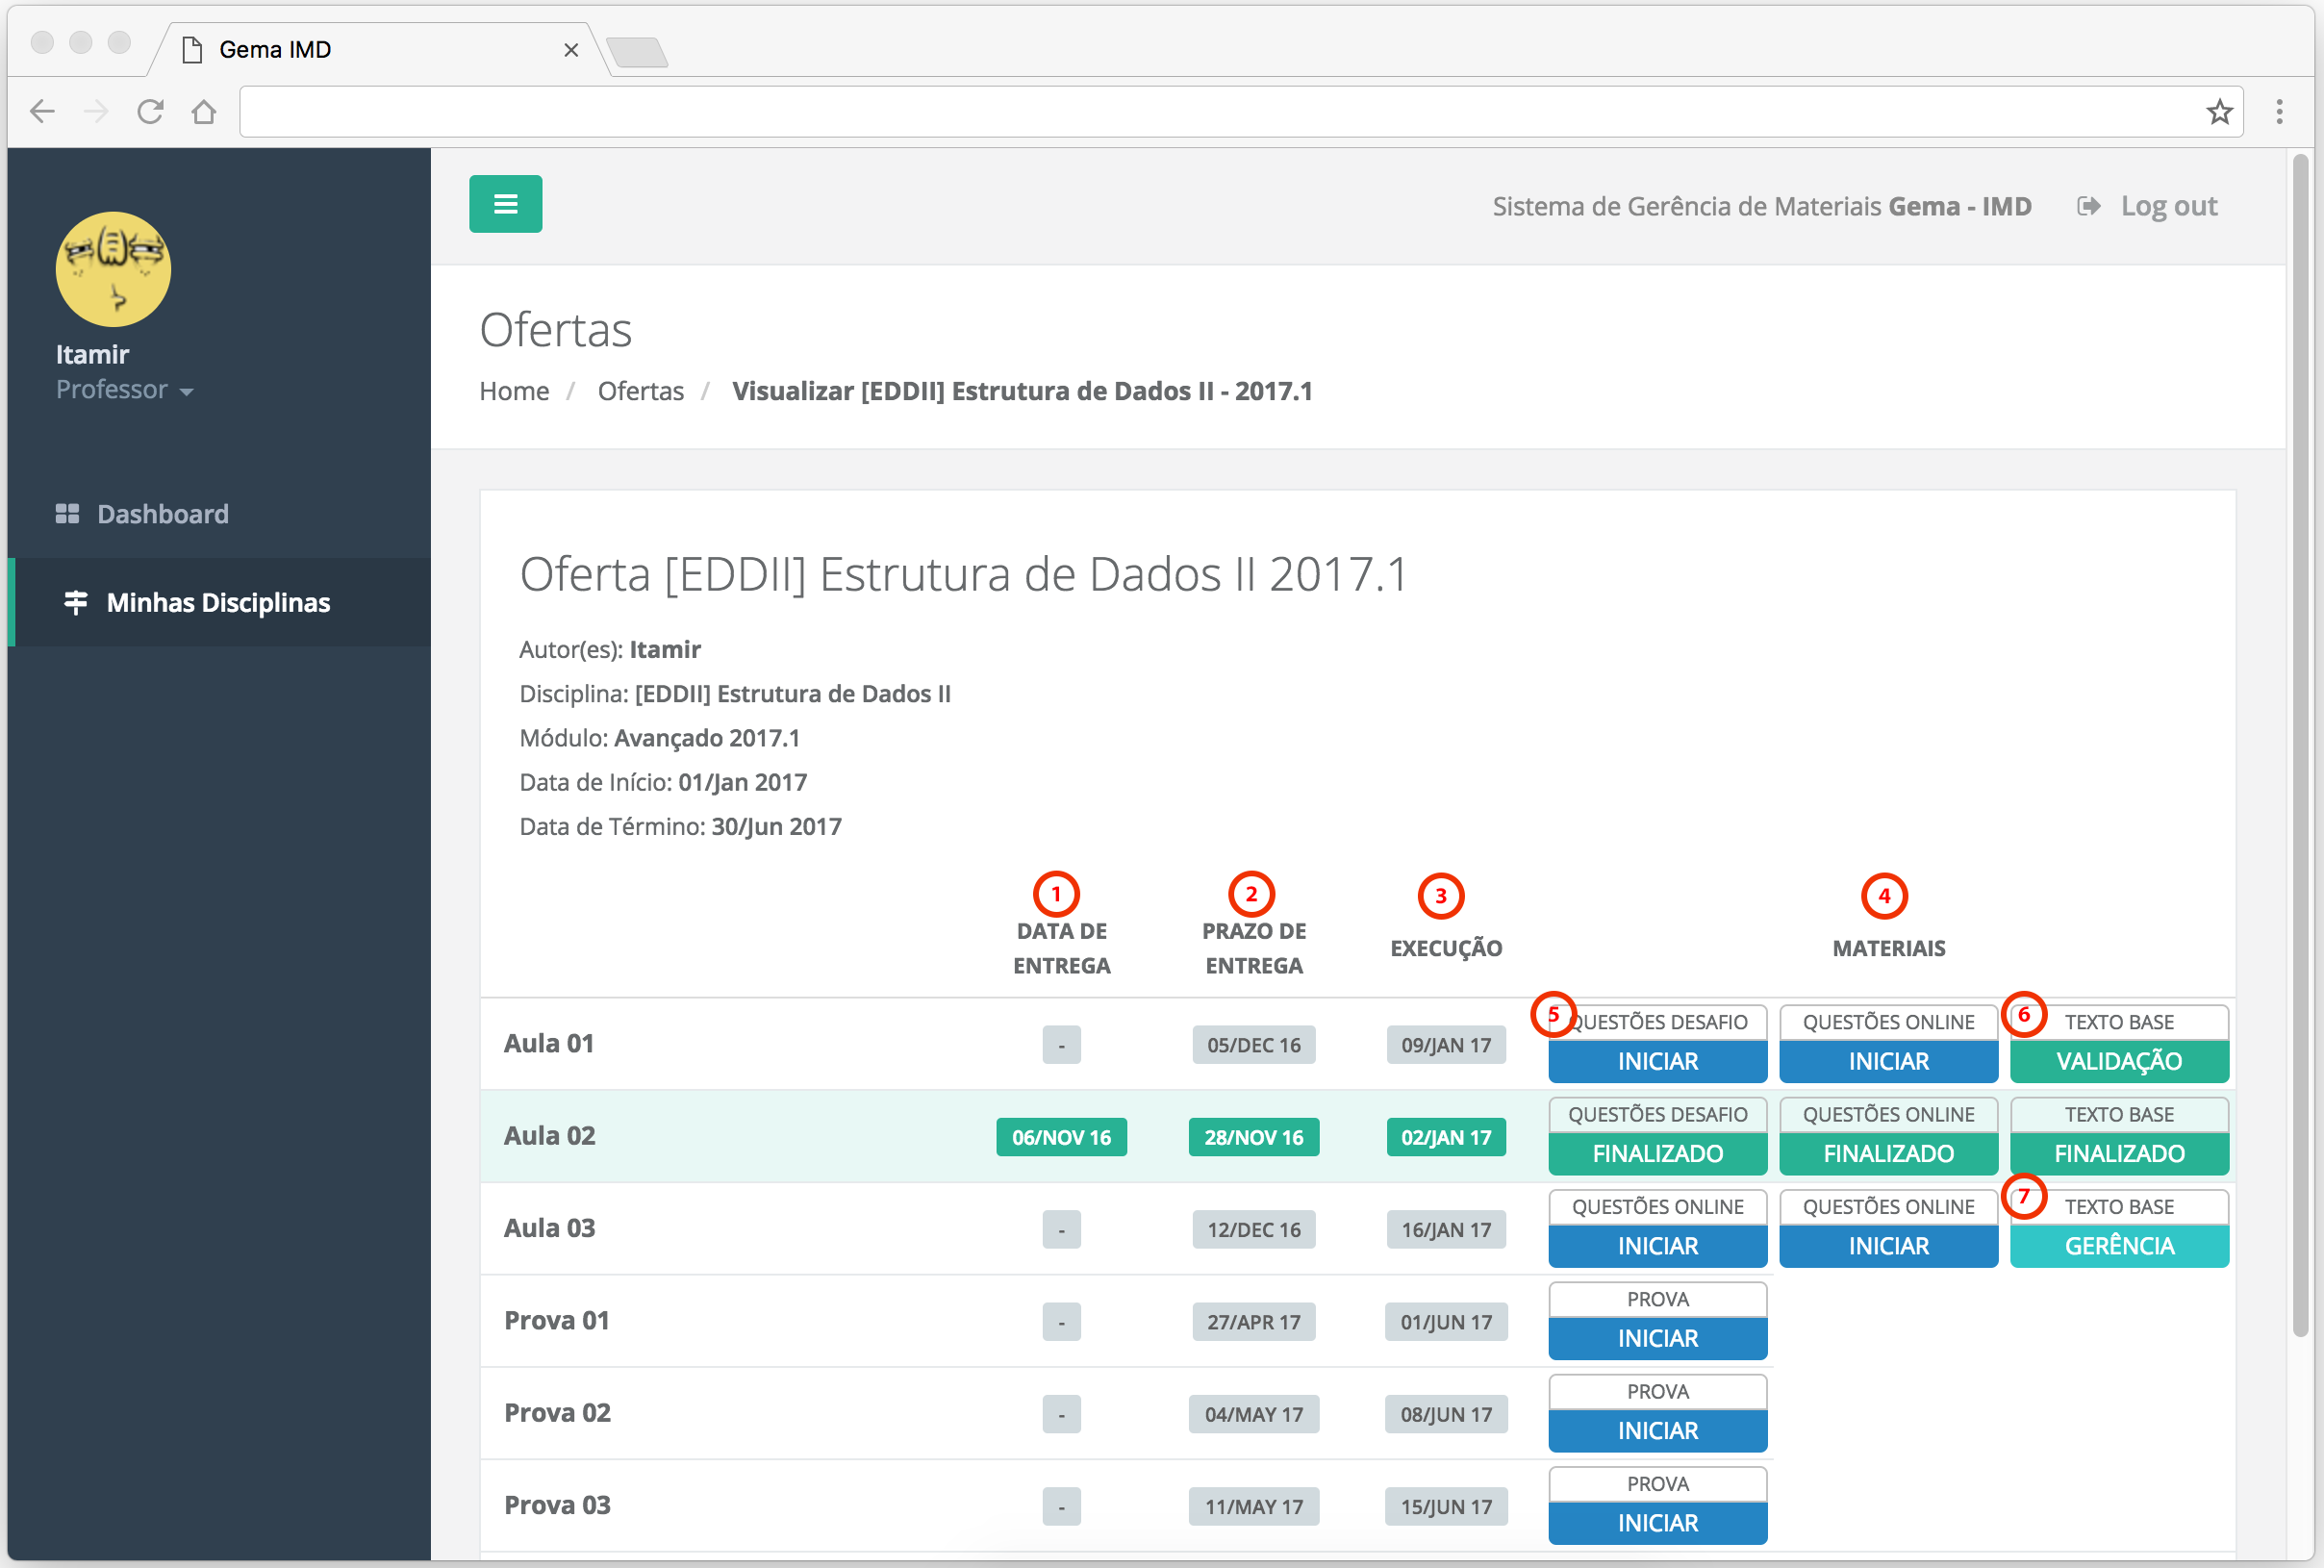
\includegraphics[width=1.0\textwidth]{Screens/OffersShow.png}
      \caption{Tela de Visualização de Oferta}
       \label{fig:OffersShow}
\end{figure} 

Além das informações gerais como lista de autores, disciplina, módulo e datas de início e término, a tela de visualização da oferta mostra os estados de cada artefato e seus materiais. Logo abaixo descrevemos os elementos com os marcadores da figura \hyperref[fig:OffersShow]{\ref{fig:OffersShow}}.

Nessa apresentação é possível visualizar a data de entrega (calculada com base na data de entrega do último material após todos terem sido entregues), prazo de entrega e execução de cada aula.

\begin{enumerate}
	\item Para cada artefato, os valores na coluna \textbf{DATA DE ENTREGA} são atribuídos como a data de entrega do último material após todos serem entregues.
	\item A coluna \textbf{PRAZO DE ENTREGA} representa a data máxima para entrega de todos os materiais de cada artefato.
	\item A coluna \textbf{EXECUÇÃO} representa a data máxima para finalização de todos os materiais de cada artefato.
	\item As colunas de \textbf{MATERIAIS} agrupam individualmente cada material do artefato através de botões arranjados com o nome e o estado atual no fluxo de produção.
	\item Materiais cujo fluxo não foi iniciado possuem em seu estado a chamada INICIAR com fundo azul escuro, sugerindo para o autor a ação de iniciar o fluxo de produção.
	\item Materiais em período de validação, finalização ou finalizados possuem em suas chamadas os títulos VALIDAÇÃO, FINALIZAÇÃO e FINALIZADO respectivamente. A cor de fundo usada é o verde.
	\item Para materiais o fluxo de produção em curso, a chamada representa a etapa no qual este se encontra. A cor de fundo usada é o azul claro.
\end{enumerate}

Dando continuidade ao processo de validação, ao clicar no botão de validação para o texto base da aula 01 na tela da figura \hyperref[fig:OffersShow]{\ref{fig:OffersShow}}, o usuário é direcionado ao formulário a seguir.

\begin{figure}[H]
\centering
     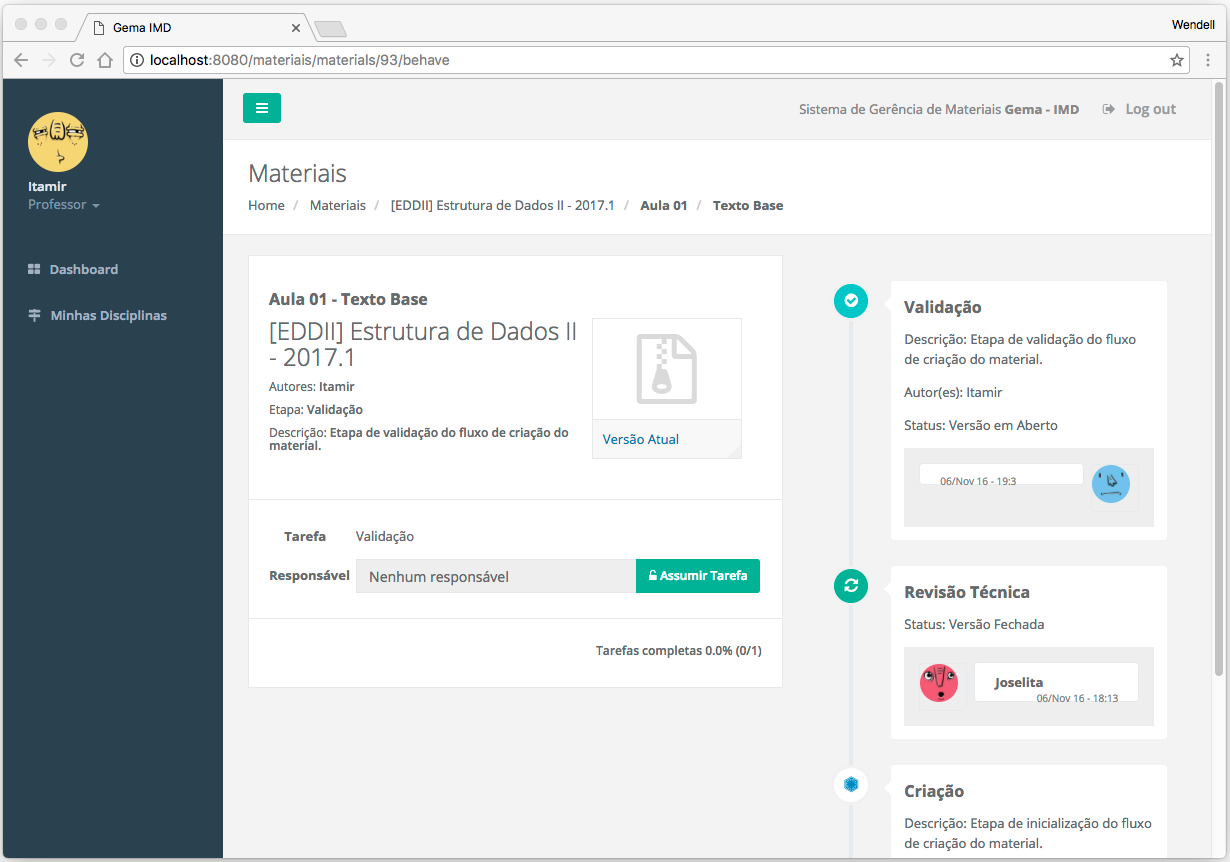
\includegraphics[width=1.0\textwidth]{Screens/EndFlow.png}
      \caption{Tela do Passo 1 para Validação do Fluxo de Material}
       \label{fig:endFlow}
\end{figure} 

A etapa de validação é semelhante as demais etapas do fluxo de produção, nela o autor sinalizar para os possíveis outros autores que ele é o responsável em validar aquele material através do botão \textbf{Assumir Tarefa} e adicionar uma observação para conclusão da atividade. Esses dois passos são representados dos passos 1 e 2 das figuras \hyperref[fig:endFlow2]{\ref{fig:endFlow2}} e \hyperref[fig:endFlow3]{\ref{fig:endFlow3}}.

\begin{figure}[H]
\centering
     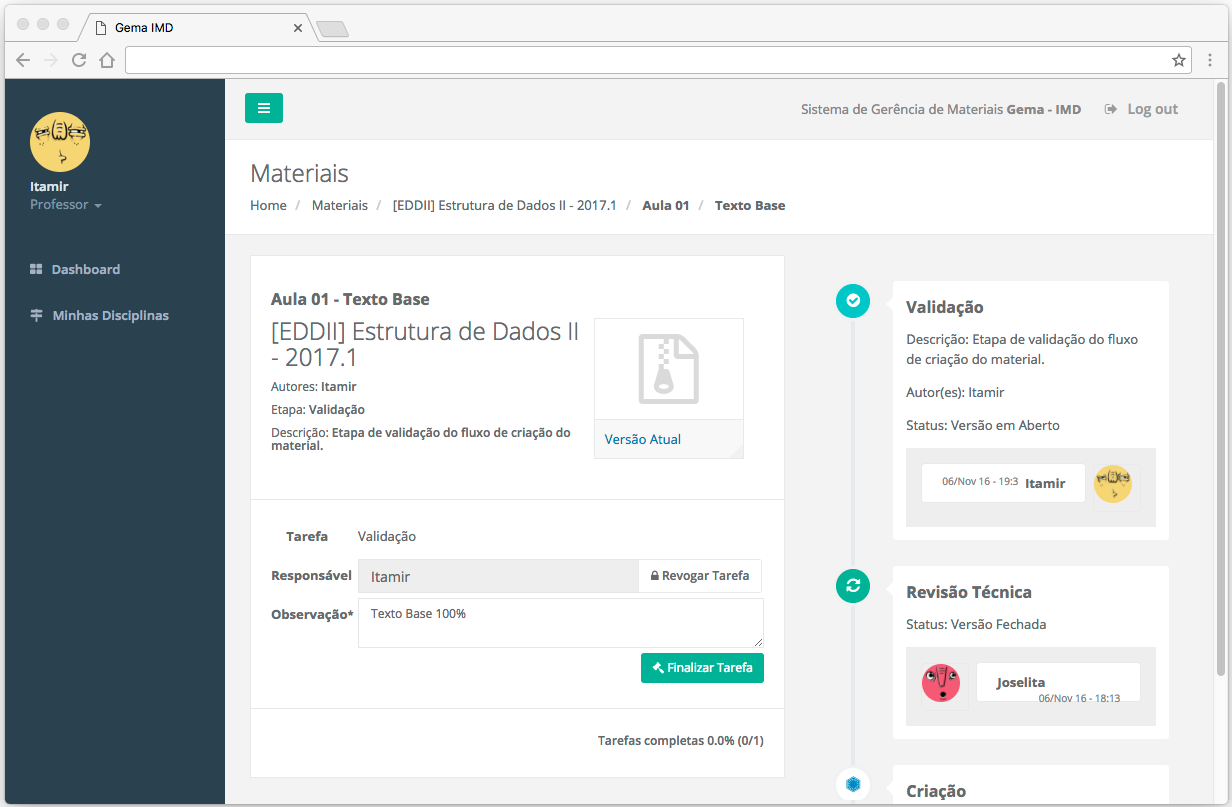
\includegraphics[width=1.0\textwidth]{Screens/EndFlow2.png}
      \caption{Tela do Passo 2 para Validação do Fluxo de Material}
       \label{fig:endFlow2}
\end{figure} 

\begin{figure}[H]
\centering
     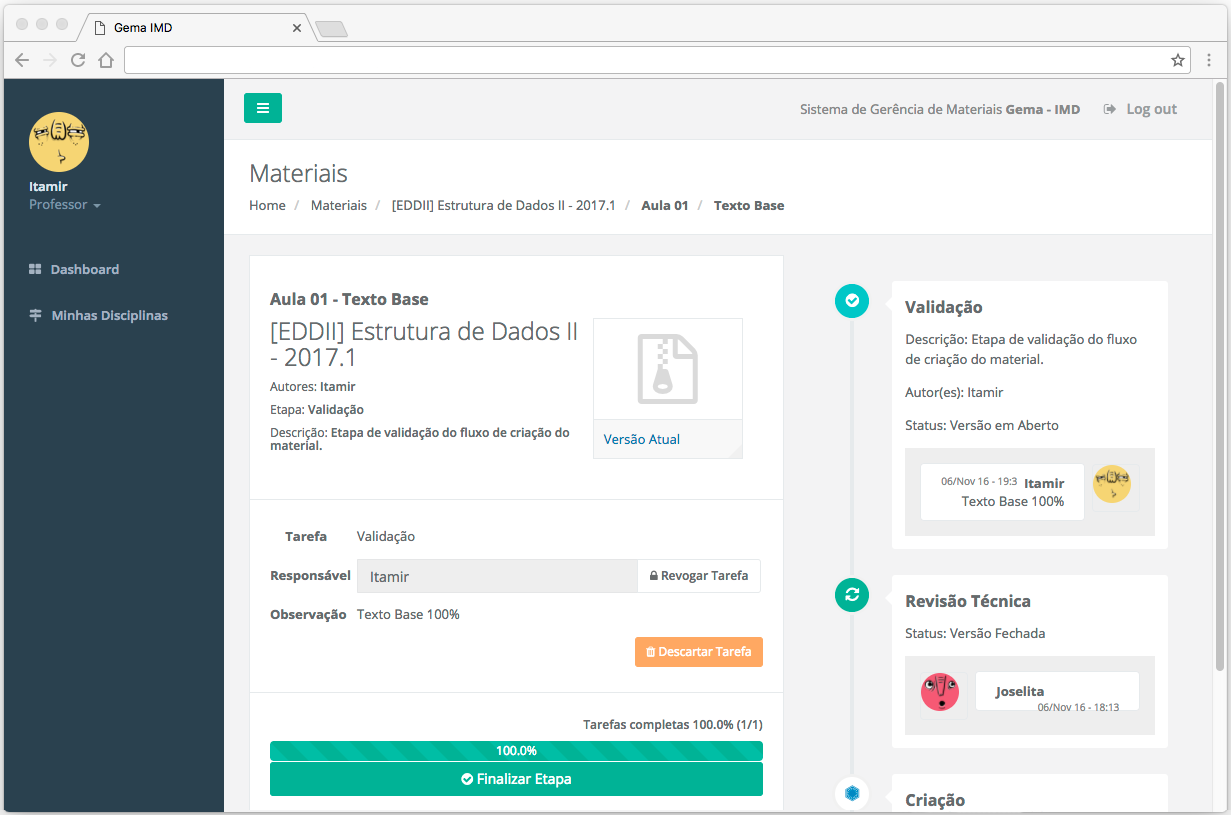
\includegraphics[width=1.0\textwidth]{Screens/EndFlow3.png}
      \caption{Tela do Passo 3 para Validação do Fluxo de Material}
       \label{fig:endFlow3}
\end{figure} 

Feita a atividade de validação do material, o autor deve finalizar a etapa usando o botão \textbf{Finalizar Etapa} do formulário (figura \hyperref[fig:endFlow3]{\ref{fig:endFlow3}}), essa ação irá acionar a tela de confirmação da figura abaixo.

\begin{figure}[H]
\centering
     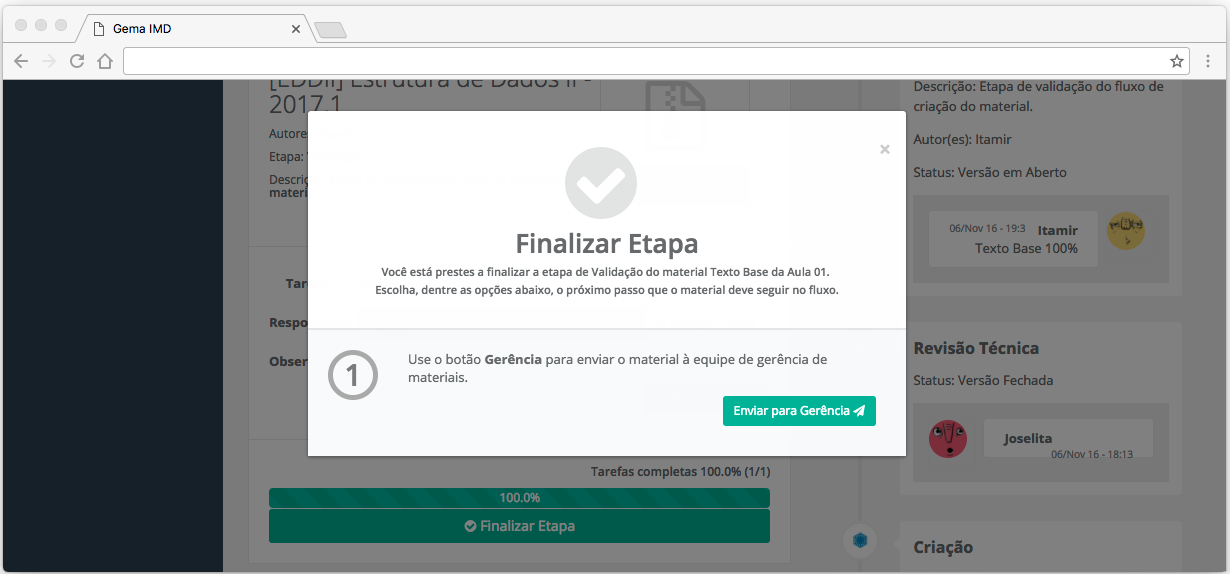
\includegraphics[width=1.0\textwidth]{Screens/EndFlow4.png}
      \caption{Tela do Passo 4 para Validação do Fluxo de Material}
       \label{fig:endFlow4}
\end{figure} 

Usar o botão \textbf{Enviar para Gerência} na tela da figura acima determina o início da segunda e última fase do processo de produção do material, a etapa de finalização.

Após autenticação no sistema, o usuário da gerência (perfil de navegação 1 da subseção \hyperref[nav_perfis]{\ref{nav_perfis}}) deve executar a etapa de finalização de forma similar à etapa de validação nos passos 1, 2 e 3 (figuras \hyperref[fig:endFlow]{\ref{fig:endFlow}}, \hyperref[fig:endFlow2]{\ref{fig:endFlow2}} e \hyperref[fig:endFlow3]{\ref{fig:endFlow3}}). Para o passo 4, a gerência possui mais controles, estes são demonstrados na tela da figura abaixo.

\begin{figure}[H]
\centering
     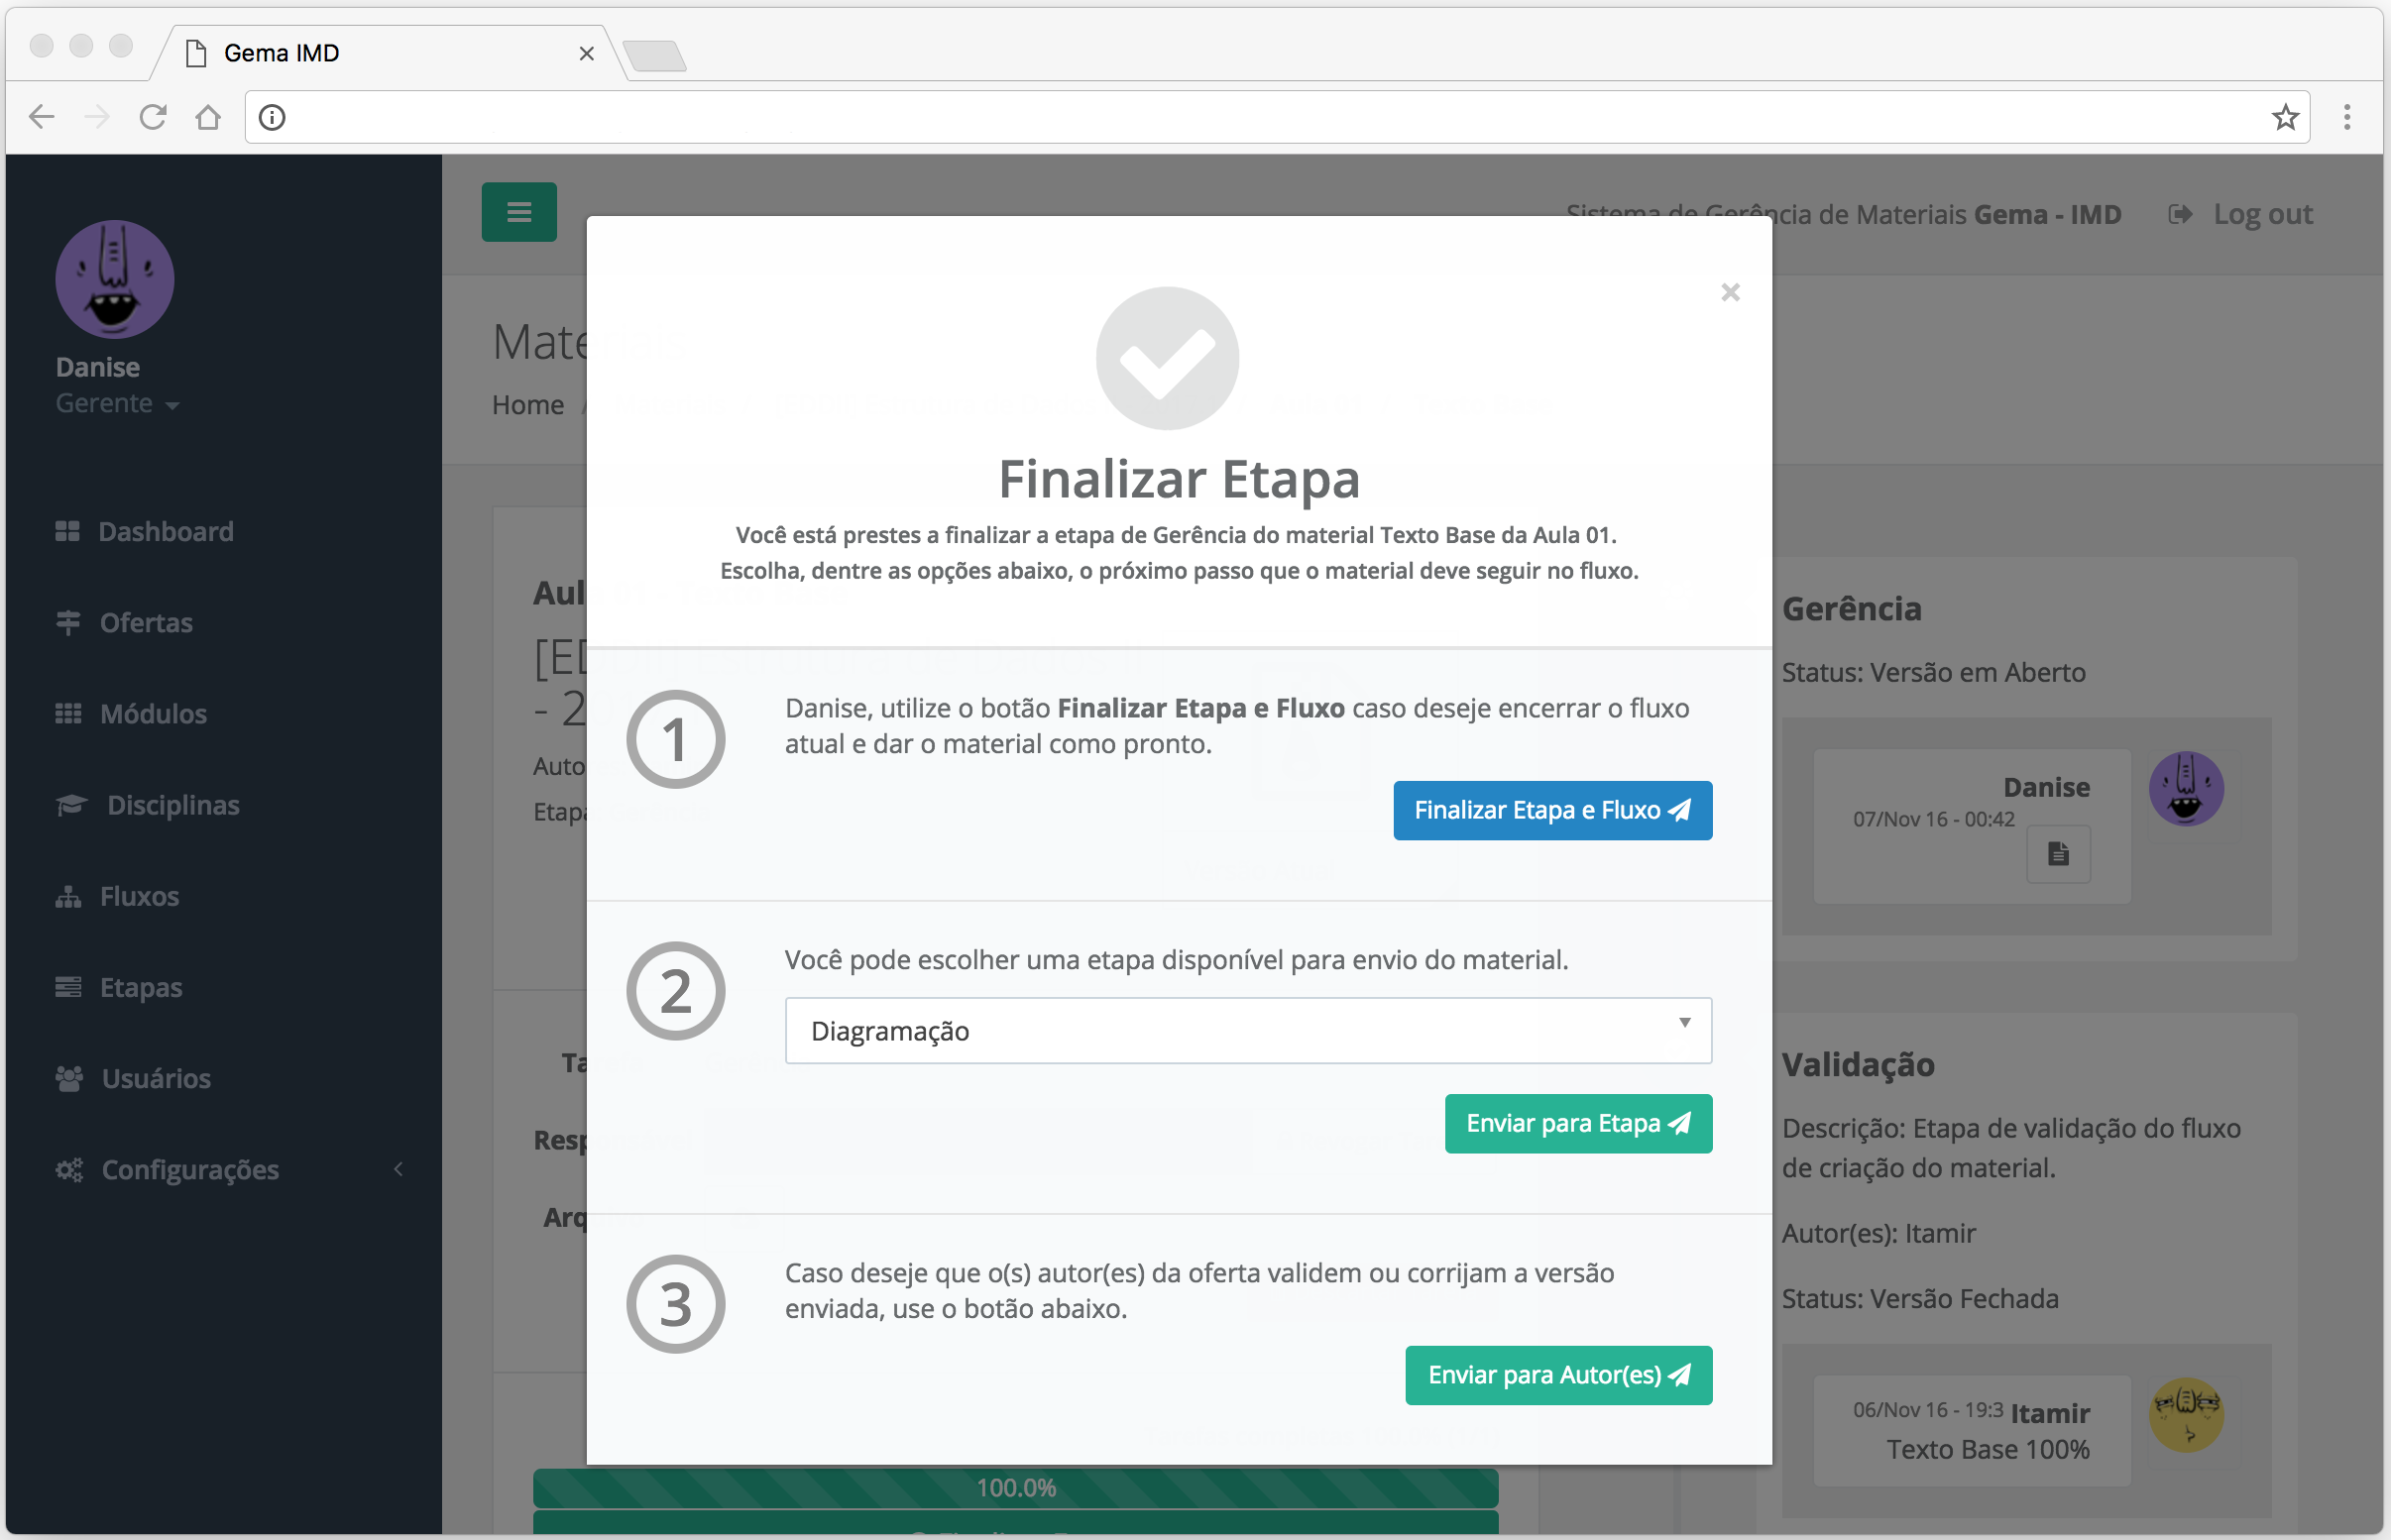
\includegraphics[width=1.0\textwidth]{Screens/EndFlow4Management.png}
      \caption{Tela do Passo 4 para Finalização do Fluxo de Material}
       \label{fig:endFlow5Management}
\end{figure} 

Na figura \hyperref[fig:endFlow5Management]{\ref{fig:endFlow5Management}}, o controle 1 representa a ação de finalização em definitivo do fluxo de produção, o 2 determina o retorno do material para equipe de produção e o último inicia uma nova fase de correção pelos autores. 

\begin{figure}[H]
\centering
     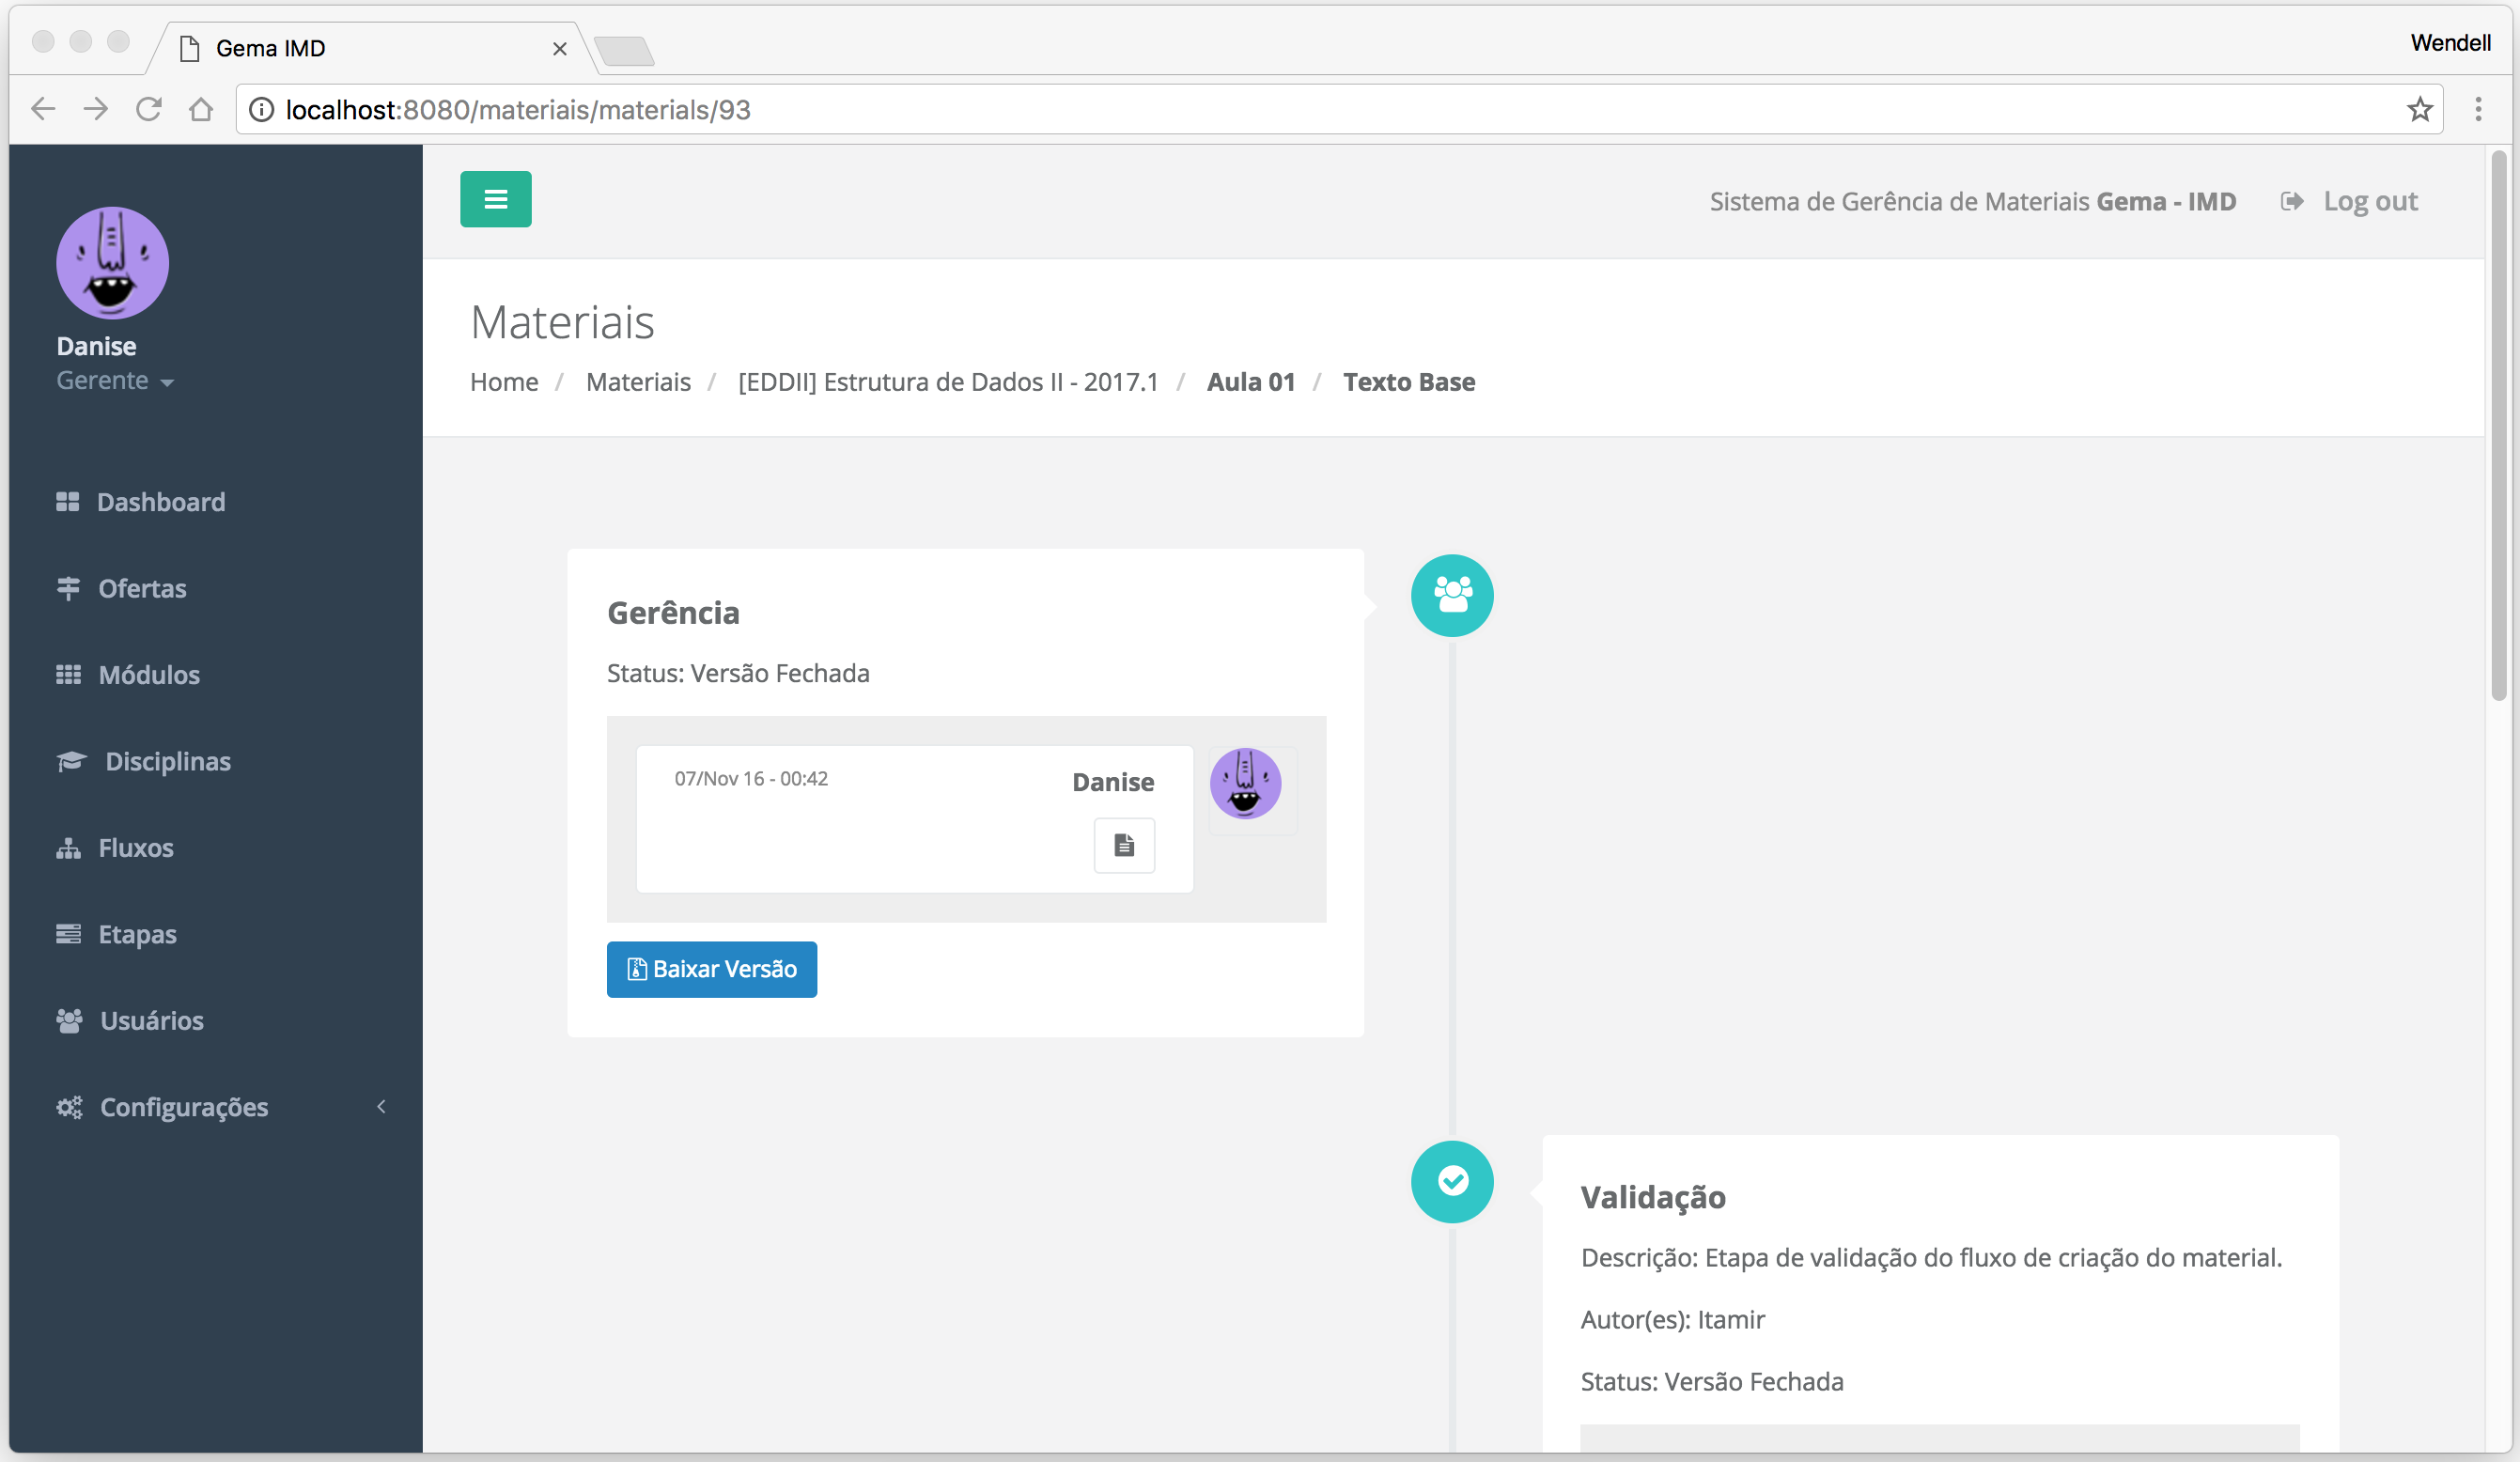
\includegraphics[width=1.0\textwidth]{Screens/MaterialTimeline2.png}
      \caption{Tela de Linha do Tempo do Material Finalizado}
       \label{fig:materialTimeline2}
\end{figure} 

Para encerrar nosso exemplo, iremos supor que o material esteja pronto e o fluxo seja finalizado. A tela da figura acima mostra a linha do tempo com os últimos passos do processo e permite a obtenção da versão final do material.

\section{Validação}

A criação da aplicação foi executada segundo duas metodologias ágeis de desenvolvimento de software. Essas metodologias são conhecidas como \textbf{Extreme Programming (XP)} e \textbf{SCRUM}.

As metodologias ágeis de desenvolvimento, no Brasil, têm gerado grande entusiasmo entre seus usuários, assim como na comunidade acadêmica. Destacam-se, principalmente, os aspectos relacionados as melhorias nos resultados que a empresa de software deseja obter, como o aprimoramento de seus processos internos e de sua estrutura organizacional (VARASCHIM, 2009). 

XP é talvez o mais conhecido e utilizado dos métodos ágeis. Utiliza boas práticas
como: desenvolvimento iterativo, envolvimento do cliente como parte da equipe, refatoração entre outros. (SOMMERVILLE, 2011)

XP prioriza a comunicação e ela é feita por diálogos presenciais constantes, estabelecendo pontos importantes do projeto de software, e dando atenção a todos os detalhes como gestos, expressões faciais, postura, tom de voz, entre outros, onde o cliente expõe suas necessidades e a equipe estima custos e prazos. Dando oportunidade de compreensão do projeto a todos os envolvidos e permitindo o melhor planejamento. (COSTA, 2011) 

A equipe de desenvolvimento lida com as mudanças de maneira natural, busca se adaptar as mudanças com coragem e segurança, confiando nos mecanismos de proteção. (COSTA, 2011) 

O termo \textbf{Extreme Programming} existe pra enfatizar iterações intensas de programação em períodos curtos de tempo objetivando a entrega e a validação por parte dos clientes.

O SCRUM é um modelo ágil de processo que foi desenvolvido por Jeff Sutherland e por sua equipe no início da década de 1990 (PRESSMAN 2006). Originalmente, o SCRUM foi desenvolvido para ser implementado em equipes de desenvolvimento de produtos de software. Porém, pode ser utilizado por qualquer empresa que necessite implementar processos de gerenciamento de projetos, tais como agências de publicidade, projetos de arquitetura, bancos, etc. (SILVA ET AL 2010).

O SCRUM baseia-se em seis características: flexibilidade dos resultados; flexibilidade dos prazos; times pequenos; revisões freqüentes; colaboração; orientação a objetos (SCHWABER 1995). Este método não requer ou fornece qualquer técnica específica para a fase de desenvolvimento, apenas estabelece conjuntos de regras e práticas gerenciais que devem ser adotadas para o sucesso de um projeto. (CARVALHO E MELLO 2009)

Foi sob a luz das metodologias citadas que ciclos foram elaborados para suprir a necessidade do desenvolvimento de funcionalidades particionadas que puderam ser validadas junto com os envolvidos. As práticas para essas validações serão descritas a seguir.

\subsection{Product Backlog}

O Product Backlog é uma prática do \textbf{XP} que prevê uma lista contendo todas as funcionalidades desejadas para o produto. Essa lista é elaborada incrementalmente pelo Product Owner, nome dado a pessoa responsável por essa tarefa.

De início, o Product Backlog foi feito com tudo o que se mostrou óbvio nos primeiros contatos e, com o tempo, essa lista foi mudando e crescendo à medida que se aprendeu mais sobre os usuários e o produto.

\subsection{Sprint Backlog}

Tendo em mãos o Product Backlog, períodos de 21 dias foram estabelecidos para a implementação de agrupamentos de funcionalidades priorizadas no que chamamos de Sprint Backlog. Cada período desse é chamado de Sprint e as funcionalidades são escolhidas estrategicamente para que possam ser validadas ao final do ciclo.

Da metade pro fim do desenvolvimento, o período de cada Sprint foi reduzido a 14 e 7 dias, o que representou a implementação de funcionalidades mais compactas e validações mais frequentes.

\subsection{Reuniões Presenciais}

Finalmente, para validar todas as funcionalidades desenvolvidas em cada ciclo, reuniões presenciais com os usuários foram feitas. 

As reuniões aconteceram em períodos de 21, 14 e 7 dias. O intervalo foi encurtado a medida que o projeto foi evoluindo, isso garantiu confirmações e retificações mais pontuais em funcionalidades críticas ao sistema. O processo também beneficiou o desenvolvimento ao passo que diminuiu drasticamente a necessidade de retrabalho e proporcionou versões da aplicação em um ambiente de testes para que os usuários pudessem continuamente verificar o que estava sendo adicionado.

Reuniões presenciais se justificam nas metodologias apresentadas pois, nesses encontros, é possível imergir cada vez mais no contexto em que a aplicação se mostra solução de um problema. Isso soma características de usuário ao desenvolvedor e trás os usuários cada vez mais para dentro do time de desenvolvimento. Concluímos então que, além das justificativas apresentadas nas metodologias, do início ao fim do projeto, a troca de informações e experiências encontradas nessa prática fundamentaram a sua escolha.



	
	% Capitulo 3: Terceiro capítulo (arquivo Includes/Cronograma.tex)
	%% SiMate

\chapter{Cronograma}
		
	% Conclusões
	\chapter{Conclusões}

\section{Considerações e Conclusões}

O \textbf{Gema} é uma solução de software desenvolvida com o intuito de potencializar as atividades que permeiam a gestão de produção de materiais multimídia. O uso dela reduz os gastos com alternativas de controle manual e aumenta a eficácia e visibilidade no cumprimento de cada etapa do processo. Tarefas primordiais como as de notificação de prazos são removidas da responsabilidade da equipe de gerência e determinam comportamentos de sistema, sendo esses executados com precisão diária a garantir o recebimento de cada alerta e aviso por parte dos usuários.

No que se diz respeito à arquitetura usada, o \textbf{Gema} se baseia no Framework de desenvolvimento do IMD, dessa maneira, o trabalho aqui realizado serve de documentação em uma linguagem comum para os desenvolvedores do setor de desenvolvimento do instituto. Os componentes produzidos na aplicação possuem propriedades para serem facilmente estendidos e reutilizados, buscando trazer importantes benefícios para o processo de manutenção do sistema.

As aplicações dos conceitos da engenharia de software e de projeto de interface de usuário nesse estudo foram importantes para que o desenvolvimento fosse realizado acentuando os aspectos de usabilidade e garantindo a capacidade de expansão do sistema. 

O especificação do \textbf{Gema} trouxe benefícios tanto para o desenvolvimento da aplicação  quanto prospecta a publicação base para uso e manutenção. Ao término desse trabalho, o sistema atua no Setor de Produção Multimídia cumprindo suas expectativas e abrindo a visão dos usuários para a constante evolução do processo produtivo. 

\section{Trabalhos Futuros}

Utilizando o \textbf{Gema}, é possível executar fluxos genéricos dos materiais de caráter didático que compõem as ofertas de disciplina. A Oferta representa o modelo base da necessidade inicial do setor, mas não deve ser o único a compor o sistema. Dessa maneira, o primeiro dos trabalhos futuros se justifica na extensão do sistema com a implementação de modelos que determinam a produção de materiais para eventos, cursos e demais situações que fazem ou farão parte do escopo de produção do instituto.

%Atualmente, o fluxo de produção multimídia que acontece no sistema começa após a elaboração da primeira versão do material, isto ocorre pois o sistema não suporta o gerenciamento de conteúdo multimídia como criação e edição de textos, imagens, áudio e vídeo. Dado que ainda não existe abertura para o suporte eficaz à gerência de imagens, áudio e vídeo na WEB, mas alternativas sólidas para a edição de documentos de texto já são passivas de implementação, uma das funcionalidades pretendidas para o \textbf{Gema} é a de gestão de conteúdo de documentos com ferramentas de configuração de estilo, edição multiusuário em tempo real, interação através de comentários, controle de versão de mudanças e exportação do conteúdo para as extensões comumente usadas.

Um das maiores preocupações no desenvolvimento da ferramenta foi a de evidenciar as necessidades do usuário. A visualização das informações pertinentes a cada etapa do fluxo são realçadas para auxiliar o usuário a cumprir o processo da maneira mais eficaz possível. Mantendo essa abordagem, pretendemos implementar mecanismos estatísticos com métricas e produção de relatórios para que se possa analisar o sistema pós execução dos fluxos. Esses mecanismos servirão para que os gerentes possam visualizar o desenvolver dos autores e equipes em cada nincho de produção.
 
Outra face do sistema que enfatiza a visualização do que está acontecendo no fluxo é a de notificação. Esse mecanismo se mostra sensível ao passo que precisa cumprir duas funções cruciais: a de carregar o que se quer informar e a de ser eficiente, ou seja, ser atrativo para que o usuário busque e entenda a informação passada. Pela importância da efetividade encontrada no cumprimento dessas funções, aperfeiçoá-las é um dos objetivos planejados nos trabalhos futuros. 
 
Finalmente, o sistema \textbf{Gema} busca cada vez mais a integralização na plataforma de aplicações do Instituto Metrópole Digital, sendo assim, planejamos realizar essa ponte de comunicação entre os sistemas para que, fornecendo e colhendo dados, se possa potencializar os serviços oferecidos.
 
 
 
 
 
	
	% Bibliografia (arquivo Chapters/Referencias.bib)
	%\bibliography{Chapters/Referencias}
	%\bibliographystyle{abnt-alf}
	
	% Apêndice A (arquivo Includes/ApendiceA)
	%\include{Chapters/ApendiceA}
	
	% Anexo A (arquivo Includes/AnexoA)
	%\include{Chapters/AnexoA}
	
	% Página em branco
	\newpage

\end{document}